% ------------------------------------------------------------------------------
% Methods Overview
% ------------------------------------------------------------------------------

\chapter{Methods Overview}\label{chap:methods}

	%Uma vez que expressões analíticas para o problema só são possíveis em algumas situações onde a geometria do problema é bem delimitada, é necessário utilizar abordagens numéricas para resolver o problema inverso. Este capítulo tem o objetivo de fazer uma ampla revisão cobrindo tanto as formas de discretização, necessárias para a implementação computacional, como para as formas de se obter uma solução.
	%Since analytical expressions for the problem are only possible in some situations where the problem geometry has a simple shape, it is necessary to use numerical approaches to solve the inverse problem. This chapter has the objective of carrying out a wide-ranging review covering both forms of discretization (necessary for the computational implementation) and the ways to obtain a solution.
	
	%Primeiro, será apresentado um esquema geral do problema a partir de definição bem comum do domínio do problema. Na sequência, serão discutidas as diversas abordagens de discretização das equações para o problema bidimensional. As metodologias para abordagem linear para o problema são apresentadas em seguida. Embora essa dissertação tenha como objetivo o problema não-linear, muitos métodos adotam a versão linearizada tanto para inicializações como pequenos passos na busca. A duas classes de métodos quantitativos são apresentadas e discutidas na sequência, i.e., os métodos determinísticos e os estocásticos. A proposta destas duas seções é fazer uma revisão bibliográfica, elencando os principais métodos, estratégias e ideias propostas na literatura. Além dessas classes, foi dado destaque também a aplicação de métodos Deep-Learning que tem recebido muita atenção na literatura recentemente. Por fim, uma breve conclusão destacando os principais pontos do capítulo é apresentada.
	%First, a general outline of the problem will be presented in Section \ref{chap:methods:definition} from a standard definition of the problem domain. Following, in Section \ref{chap:methods:discretization}, the various approaches to discretization of the equations for the two-dimensional problem will be discussed. The methodologies for a linear approach to the problem are presented in Section \ref{chap:methods:linear}. Regularization methods are also used after linearization of the integral equation and are presented in Section \ref{chap:methods:regularization}. Section \ref{chap:methods:qualitative} presents methods for cases when only the shape of the scatterers are necessary to recover, i.e., qualitative methods. On the other hand, the two classes of quantitative methods are presented and discussed in the sequence, i.e., the deterministic (Section \ref{chap:methods:deterministic}) and stochastic ones (Section \ref{chap:methods:stochastic}). The purpose of these two sections is to present a bibliographic review, listing the main methods, strategies and ideas proposed in the literature. In addition to these classes, emphasis was also placed on applying Deep-Learning methods (Section \ref{chap:methods:deep}), which has recently received much attention in the literature. Lastly, a brief conclusion highlighting the main points of the chapter is presented in Section \ref{chap:methods:conclusion}.
	
	Since the inverse problem is ill-posed and nonlinear, analytical approaches are usually not considered. Due to such complexity numerical approaches are necessary to obtain a solution. This chapter aims to provide a comprehensive review of the various methods and techniques used to address the inverse problem.
	
	Section \ref{chap:methods:definition} presents a general overview of the problem domain, followed by a discussion on the different approaches to discretization of the equations for the two-dimensional problem in Section \ref{chap:methods:discretization}. In Section \ref{chap:methods:linear}, methodologies for a linear approach to the problem are presented. Regularization methods, which are used after linearization of the integral equation, are discussed in Section \ref{chap:methods:regularization}.
	
	Section \ref{chap:methods:qualitative} focuses on qualitative methods, which are used when only the shape of the scatterers needs to be recovered. The two classes of quantitative methods are presented in the subsequent sections, i.e., deterministic methods in Section \ref{chap:methods:deterministic} and stochastic methods in Section \ref{chap:methods:stochastic}. These sections provide a bibliographic review of the main methods, strategies, and ideas proposed in the literature.
	
	The chapter also emphasizes the application of Deep-Learning methods, which has recently gained significant attention in the literature, as discussed in Section \ref{chap:methods:deep}. Lastly, a brief conclusion is presented in Section \ref{chap:methods:conclusion} to summarize the main points covered in the chapter.
	

	\section{Domain Definition}\label{chap:methods:definition}
	
	 	%Toda a investigação conduzida neste trabalho pressuporá um problema bidimensional TMz com materiais lineares, isotrópicos, não-dispersivos e não-magnéticos. Portanto, \eqref{eq:2:2d:4}-\eqref{eq:2:2d:8} serão as equações que descreverão as relações entre campos, fonte e meio. No entanto, antes de adentrar nas metodologias, é necessário definir adequadamente o domínio do problema, i.e., a geometria dos espaços onde serão definidas todas as variáveis e constantes. Essas definições serão o referencial de todas as metodologias descritas nesse trabalho.
	 	All the research conducted in this work will presuppose a two-dimensional TMz problem with linear, isotropic, non-dispersive and non-magnetic materials. Therefore, \eqref{eq:2:2d:4}-\eqref{eq:2:2d:8} will be the equations that will describe the relationships between fields, source and medium. However, before entering the methodologies, it is necessary to adequately define the problem domain, i.e., the geometry of the spaces where all variables and constants are defined. These definitions will be the foundation for all the methodologies described in this work.
	 	
	 	%A Figura \ref{fig:3:domaindefinition} descreve a geometria do problema. O campo espalhado $E_{z_s}$ é definido sobre um círculo centrado na origem dos eixos cartesianos cujo raio é denotado por $R_O$, e o ângulo, por $\theta$. Esse círculo está imerso em um meio homogêneo caracterizado pelas propriedades eletromagnéticas $\epsilon_b$, $\sigma_b$ e $\mu_b$. O vetor $\brho$ em \eqref{eq:2:2d:4}-\eqref{eq:2:2d:8} pode ser escrito como:
	 	\autoref{fig:3:domaindefinition} describes the geometry of the problem. The scattered field $E_{z_s}$ is defined over a circle centred on the origin of the Cartesian axes whose radius is denoted by $R_O$, and the angle, by $\theta$. This circle is immersed in a homogeneous medium characterized by the electromagnetic properties $\epsilon_b$, $\sigma_b$, and $\mu_b$. The vector $\brho$ in \eqref{eq:2:2d:4}-\eqref{eq:2:2d:8} can be written as:
	 	\begin{equation}
	 		\brho = R_O\cos\theta\mathbf{x} + R_O\sin\theta\mathbf{y} \label{eq:3:definition:1}
	 	\end{equation}
		\begin{figure}[!b]
			\centering
			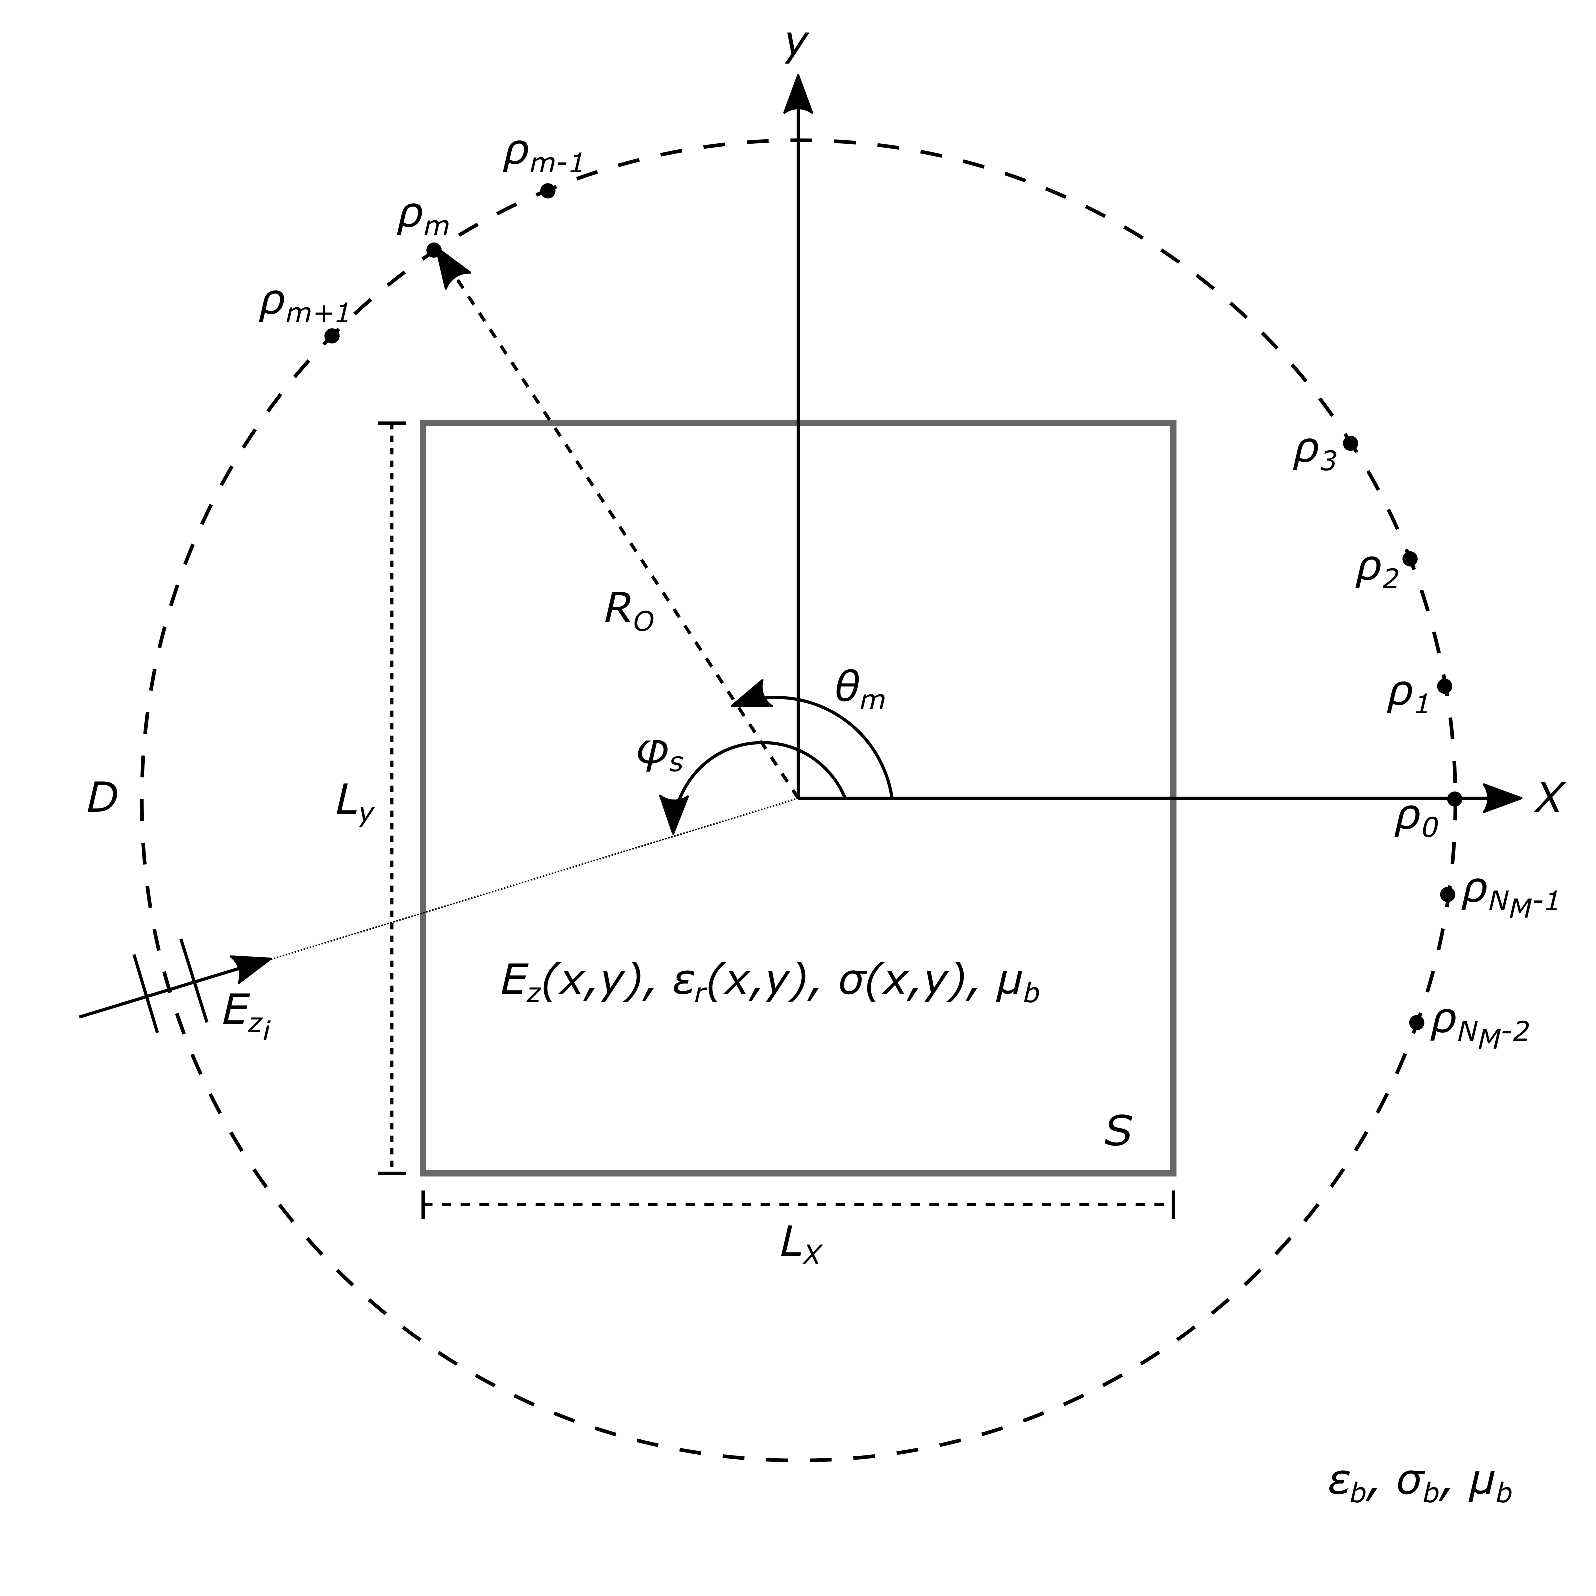
\includegraphics[width=0.5\textwidth]{./figuras/domaindefinition}
			\caption{Problem geometry.}
			\label{fig:3:domaindefinition}
		\end{figure}
 	
 		%O espaço de estados $S$ é a região retangular centrada na origem no eixo de coordenadas cujos comprimentos equivalem a $L_X$ e $L_Y$. Esta região representa a imagem a ser reconstruída, por isso, são definidas dentro delas as variáveis $E_z$, $\epsilon_r$ e $\sigma$. As duas últimas estão relacionadas à função contraste $\chi$ através de \eqref{eq:2:contrast}.
 		The state-space $S$ is the rectangular region centred at the origin on the axis of coordinate whose lengths are equal to $L_X$ and $L_Y$. This region represents the image to be reconstructed. Therefore, the variables $E_z$, $\epsilon_r$, and $\sigma$ are defined within them. The last two are related to the contrast function $\chi$ through \eqref{eq:2:contrast}.
 		
 		%Por fim, o campo incidente $E_{i_z}$ será representado por uma onda plana a qual é conhecida em todo o espaço do problema. A amplitude desta onda será denotada por $E_0$ enquanto seu ângulo de incidência em relação ao eixo cartesiano será denotado por $\phi$. Portanto, o campo incidente pode ser escrito como:
 		Finally, the incident field $E_{i_z}$ will be represented by a plane wave known throughout the problem space. The amplitude of this wave will be denoted by $E_0$, while its incidence angle concerning the Cartesian axis will be denoted by $\phi$. Therefore, the incident field can be written as:
 		\begin{equation}
 			E_{i_z}(\brho) = E_0e^{-j\mathbf{k_b}\cdot\brho} \label{eq:3:definition:2}
 		\end{equation}
 	
 		%\noindent no qual $\mathbf{k_b} = |k_b|\cos\phi\mathbf{x} + |k_b|\sin\phi\mathbf{y}$ é o vetor de número de onda. Outras formas de ondas incidentes são possíveis e toda a metodologia descrita e investigada no restante do texto é compatível.
 		\noindent where $\mathbf{k_b} = |k_b|\cos\phi\mathbf{x} + |k_b|\sin\phi\mathbf{y}$ is the wavenumber vector. Other forms of incident waves are possible and compatible with the methodology described throughout this chapter.
 		
 		%O espaço de dados $D$ será definido um domínio bidimensional conforme a seguir:
 		Data-space $D$ will be defined as a two-dimensional domain as follows:
 		\begin{equation}
 			D \coloneqq \{(\theta,\phi) : \theta, \phi \in [0,2\pi] \} \label{eq:3:definition:3}
 		\end{equation}
 	
 		%Ou seja, $D$ é uma região que relaciona os ângulos no qual o campo espalhado é definido e os de incidência. Obviamente, o campo espalhado não somente varia conforme $\theta$, mas também conforme o ângulo de incidência, uma vez que o campo espalhado é resultante da interação do campo incidente com o objeto espalhador. Por isso, a partir de agora, diremos que $E_{z_s}$ é uma função definida no domínio $D$, i.e., $E_{z_s}(\theta,\phi)$. Este tipo de definição também seria possível com ondas incidentes produzidas fontes impressas pontuais num arranjo circular, por exemplo.
 		Therefore, $D$ is a region that relates the angles in which the scattered field is defined and those of incidence. The scattered field varies according to $\theta$ and according to the angle of incidence ($\phi$) since the field scattered is the result of the interaction of the incident field with the scattering object. So, from now on, we will say that $E_{z_s}$ is a function defined in the $D$ domain, i.e., $E_{z_s}(\theta,\phi)$. This definition would also be possible with incident waves due to infinitesimal impressed sources in a circular arrangement.
 		
 		%A partir dessas definições, \eqref{eq:2:2d:4}-\eqref{eq:2:2d:8} serão reescritas como:
 		From those definitions, \eqref{eq:2:2d:4}-\eqref{eq:2:2d:8} will be rewritten as:
 		\begin{eqnarray}
 			E_{s_z}(\theta,\phi) &=& -\frac{jk_b^2}{4} \int_S dx dy~ G^D_{2D}(\theta,x,y) \chi(x,y) E_z(\phi,x,y)\label{eq:3:definition:4} \\[5pt]
 			E_z(\phi,x,y) &=& E_{z_i}(\phi,x,y) \nonumber \\[5pt]
 			&& ~~~~ - \frac{jk_b^2}{4} \int_S dx^\prime dy^\prime~ G^S_{2D}(x,y,x^\prime,y^\prime) \chi(x^\prime,y^\prime) E_z(\phi,x^\prime,y^\prime) \label{eq:3:definition:5} \\[5pt]
 			E_{s_z}(\theta,\phi) &=& -\frac{jk_b^2}{4} \int_S dxdy~ G^D_{2D}(\theta,x,y) J_{z_{eq}}(\phi,x,y) \label{eq:3:definition:6} \\[5pt]
 			\chi(x,y)E_{z_i}(\phi,x,y) &=& J_{z_{eq}}(\phi,x,y) \nonumber \\[5pt]
 			&& ~~~~~~~ + \frac{jk_b^2}{4} \chi(x,y) \int_S dx^\prime dy^\prime G^S_{2D}(x,y,x^\prime,y^\prime) J_{z_{eq}}(\phi,x,y) \label{eq:3:definition:7} \\[5pt]
 			\beta(x,y)J_{z_{eq}}(\phi,x,y) &=& R(x,y)\beta(x,y)J_{z_{eq}}(\phi,x,y) + R(x,y)\bigg[ E_{z_i}(\phi,x,y) \nonumber \\[5pt]
 			&& \left. ~~~~~~~~~~~~~ - \frac{jk_b^2}{4} \int_S dx^\prime dy^\prime~ G^S_{2D}(x,y,x^\prime,y^\prime) J_{z_{eq}}(\phi,x^\prime,y^\prime)\right] \label{eq:3:definition:8}
 		\end{eqnarray}
 	
 		%\noindent where\footnote{O leitor deve ter notado que, diferentemente de outros trabalhos na literatura \citep{chen2017}, aqui utilizaremos a letra $D$ para a região do campo espalhado e a letra $S$ para a região da imagem. Esta escolha foi feita para que o sobrescrito de $G_{2D}$ indique se a equação é a dados ou de estados.}:
 		\noindent where\footnote{The reader should have noticed that, unlike other works in the literature \citep{chen2017}, we will use the letter $D$ for the region of the scattered field and the letter $S$ for the image region. It is a choice made so that the $G_{2D}$ superscript indicates whether the equation is data or state.}
 		\begin{eqnarray}
 			G^D_{2D}(\theta,x,y) &=&  H_0^{(2)}(k_b\sqrt{(R_O\cos\theta-x)^2+(R_O\sin\theta-y)^2}) \label{eq:3:definition:9} \\[5pt]
 			G^S_{2D}(x,y,x^\prime,y^\prime) &=&  H_0^{(2)}(k_b\sqrt{(x-x^\prime)^2+(y-y^\prime)^2}) \label{eq:3:definition:10}
 		\end{eqnarray}
 	
 		The choice for such geometry is to be as simple as possible since the intention is to avoid any influence that any specific characteristic can perform. The advantage is that it is simpler for the definition of classical discretization formulas. On the other hand, it may not represent most of the real problems. However, this is not the goal of the thesis.
 	
 	\section{Discretization}\label{chap:methods:discretization}
 	
 		%Em situações práticas, o campo espalhado $E_{z_s}$ é conhecido somente em um conjunto de pontos em $D$. Além disso, para que \eqref{eq:3:definition:4}-\eqref{eq:3:definition:8} sejam resolvidas numericamente, é necessário adotar algum tipo de discretização. No contexto de métodos numéricos para equações diferenciais, a discretização é feita a partir da definição da forma fraca e forte das equações \citep{liu2009meshfree}. Um exemplo de metodologia baseado na forma forte é o Método das Diferenças Finitas onde as derivadas são aproximadas por diferenças entre valores nodais finitos \citep{taflove2005computational}. Já em relação à forma fraca, existe uma classe de métodos baseados no ponderamento dos resíduos das equações. É o chamado Método dos Resíduos Ponderados (MWR) \citep{fletcher1984computational}. Nestes métodos, para uma dada equação diferencial:
 		In practical situations, the scattered field $E_{z_s}$ is known only at a set of points in $D$. Furthermore, it is necessary to adopt some discretization to solve \eqref{eq:3:definition:4}-\eqref{eq:3:definition:8} numerically. In the context of numerical methods for differential equations, the discretization is made either from the weak or from the strong forms of the equations \citep{liu2009meshfree}. An example of a methodology based on the strong form is the Finite Difference Method, where the derivatives are approximated by differences between finite nodal values \citep{yee1966numerical,taflove2005computational}. Regarding the weak one, there is a class of methods based on weighting the residuals of the equations. It is called the Method of Weighted Residuals (MWR) \citep{fletcher1984computational}. In these methods, for a given differential equation:
 		\begin{equation}
 			\mathcal{K}\{u\} = 0 \label{eq:3:discretization:0}
 		\end{equation}
 	
 		%\noindent a solução aproximada $u_a$ é escrita da seguinte forma:
 		\noindent the approximate solution $u_a$ is written as follows:
 		\begin{equation}
 			u_a(\mathbf{r}) = u_0(\mathbf{r}) + \sum\limits_{j=1}^N a_j\psi_j(\mathbf{r}) \label{eq:3:discretization:1}
 		\end{equation}
 	
 		%\noindent onde $u_0$ é uma função que atenda as condições de contorno, $a_j$ são constantes desconhecidas e $\psi$ são funções analíticas geralmente chamadas de funções de tentativa. A função resíduo $R_{u_a}$ é definida em termos da aplicação desta solução aproximada em \eqref{eq:3:discretization:0}, i.e.:
 		\noindent where $u_0$ is a function that satisfies the boundary conditions, $a_j$ is an unknown constant, and $\psi$ are analytical functions usually called trial functions. The residual function $R_{u_a}$ is defined in terms of the application of this approximate solution in \eqref{eq:3:discretization:0}, i.e.:
 		\begin{equation}
 			\mathcal{K}\{u_a\} = R_{u_a} \label{eq:3:discretization:2}
 		\end{equation}
 	
 		%Desta forma, o Método dos Resíduos Ponderados se baseia em determinar os coeficientes $a_j$'s através da solução do conjunto de equações:
 		Hence, MWR is based on determining the coefficients $a_j$'s by solving the set of equations:
 		\begin{equation}
 			\langle R_{u_a}, w_k(\mathbf{r}) \rangle = 0,~ k=1,\cdots,N \label{eq:3:discretization:3}
 		\end{equation}
 	
 		%\noindent onde $w_k$ são funções analíticas conhecidas como funções de peso ou funções de teste. Essas funções precisam ser independentes entre si. Além disso, se elas fazem parte de um conjunto completo de funções, quando $N$ tende ao infinito, isto equivale dizer que $R_{u_a}$ tem de ser ortogonal para cada membro do conjunto completo de funções. No entanto, isto também implica que $R_{u_a}$ converge para zero na média.
 		\noindent where $w_k$'s are analytical functions known as weight functions or test functions. These functions must be independent of each other. Furthermore, if they are part of a base, when $N$ tends to infinity, this is equivalent to saying that $R_{u_a}$ must be orthogonal for each member of the base functions. However, this also implies that $R_{u_a}$ converges to zero on average.
 		
 		%De maneira similar, nós podemos aplicar o MWR à \eqref{eq:3:definition:4}. Considerando o problema não-linear, onde $E_z$ e $\chi$ são desconhecidos, as seguintes aproximações serão feitas:
 		Similarly, we can apply MWR to integral equations such as \eqref{eq:3:definition:4}. Considering a nonlinear problem, where $E_z$ and $\chi$ are unknown, the following approximations will be made:
 		\begin{eqnarray}
 			\chi(x,y) &\approx& \sum\limits_{i=1}^{N_I}\sum\limits_{j=1}^{N_J} a_{ij} f^{(x)}_i(x) f^{(y)}_j(y) \label{eq:3:discretization:4} \\[5pt]
 			E_z(\phi,x,y) &\approx& \sum\limits_{p=1}^{N_P}\sum\limits_{q=1}^{N_Q}\sum\limits_{r=1}^{N_R} b_{pqr} g^{(x)}_{p}(x) g^{(y)}_{q}(y) g^{(\phi)}_r(\phi) \label{eq:3:discretization:5} 
 		\end{eqnarray}
 	
 		%As funções $f^{(x)}$, $f^{(y)}$, $g^{(x)}$, $g^{(y)}$ e $g^{(\phi)}$ são as funções de tentativa enquanto os coeficientes $a$ e $b$ são desconhecidas. A partir dessas definições, podemos escrever o seguinte conjunto de equações:
 		The functions $f^{(x)}$, $f^{(y)}$, $g^{(x)}$, $g^{(y)}$ and $g^{(\phi)}$ are the trial functions while the coefficients $a$ and $b$ are unknown. They can be defined everywhere in $S$ or even locally, i.e., some portions of the state space. It should be noted that we are choosing the trial function formulation $f(x,y) = f^{(x)}(x)f^{(y)}(y)$, but other formulations are possible. Our choice is due our previous experience with this kind of formulation. From these definitions, we can write the following set of equations:
 		\begin{multline}
 			\iint_D E_{z_s}(\theta,\phi) w^{(\theta)}_u(\theta) w^{(\phi)}_v(\phi) d\theta d\phi = \\ -\frac{jk_b^2}{4} \sum\limits_{i=1}^{N_I}\sum\limits_{j=1}^{N_J} \sum\limits_{p=1}^{N_P}\sum\limits_{q=1}^{N_Q}\sum\limits_{r=1}^{N_R} a_{ij} b_{pqr} \iint\limits_{D} \iint\limits_{S} d\theta d\phi dxdy~ \bigg[ G^D_{2D}(\theta,x,y) \\ f^{(x)}_i(x) f^{(y)}_j(y) g^{(x)}_{p}(x) g^{(y)}_{q}(y) g^{(\phi)}_r(\phi)w^{(\theta)}_u(\theta) w^{(\phi)}_v(\phi)  \bigg], \\ u = 1,\cdots, N_U,~ v = 1,\cdots,N_V \label{eq:3:discretization:6}
 		\end{multline}
 	
 		%\noindent onde $w^{(\theta)}$ e $w^{(\phi)}$ são as funções de peso escolhidas. Essas integrais podem ser rearranjadas da seguinte forma:
 		\noindent where $w^{(\theta)}$ and $w^{(\phi)}$ are the chosen weight functions. These integrals can be rearranged as follows:
 		\begin{multline}
 			\int\limits_{0}^{2\pi}\int\limits_{0}^{2\pi} E_{z_s}(\theta,\phi) w^{(\theta)}_u(\theta) w^{(\phi)}_v(\phi) d\theta d\phi =
 			-\frac{jk_b^2}{4} \sum\limits_{i=1}^{N_I}\sum\limits_{j=1}^{N_J} \sum\limits_{p=1}^{N_P}\sum\limits_{q=1}^{N_Q}\sum\limits_{r=1}^{N_R} a_{ij} b_{pqr} \int\limits_{0}^{2\pi} d\phi~ g^{(\phi)}_r(\phi) w^{(\phi)}_v(\phi) \\ \cdot  \int\limits_{-L_X/2}^{L_X/2} dx~ f^{(x)}_i(x) g^{(x)}_{p}(x) \Bigg[ \int\limits_{-L_Y/2}^{L_Y/2}  dy~f^{(y)}_j(y) g^{(y)}_{q}(y)
 			   \bigg[ \int\limits_{0}^{2\pi} d\theta~ G^D_{2D}(\theta,x,y) w^{(\theta)}_u(\theta)  \bigg] \Bigg], \\ u = 1,\cdots, N_U,~ v = 1,\cdots,N_V \label{eq:3:discretization:7}
 		\end{multline}
 	
 		%Como é possível observar, a integral sobre $\phi$ no lado direito de \eqref{eq:3:discretization:7} pode ser separada das demais. Cada integral resulta em um escalar, por isso, cada equação em \eqref{eq:3:discretization:7} pode ser reescrita como um somatório de coeficientes:
 		As is evident, the integral on $\phi$ on the right-hand side of \eqref{eq:3:discretization:7} can be separated from the others. Each integral results in a scalar. Therefore, each equation in \eqref{eq:3:discretization:7} can be rewritten as a sum of coefficients:
 		\begin{equation}
 			\Lambda_{uv} = \sum\limits_{i=1}^{N_I} \sum\limits_{j=1}^{N_J} \sum\limits_{p=1}^{N_P} \sum\limits_{q=1}^{N_Q} \sum\limits_{r=1}^{N_R} a_{ij} b_{pqr} \Phi_{vr} \Omega_{uijpq} \label{eq:3:discretization:8}
 		\end{equation}
 	
 		%\noindent no qual:
 		\noindent in which:
 		\begin{eqnarray}
 			\Lambda_{uv} &=& \int\limits_{0}^{2\pi}\int\limits_{0}^{2\pi} E_{z_s}(\theta,\phi) w^{(\theta)}_u(\theta) w^{(\phi)}_v(\phi) d\theta d\phi \label{eq:3:discretization:9} \\
 			\Phi_{rv} &=& \int\limits_{0}^{2\pi} d\phi~ g^{(\phi)}_r(\phi) w^{(\phi)}_v(\phi) \label{eq:3:discretization:10} \\
 			\Omega_{uijpq} &=& -\frac{jk_b^2}{4} \int\limits_{-L_X/2}^{L_X/2} dx~ f^{(x)}_i(x) g^{(x)}_{p}(x) \Bigg[ \int\limits_{-L_Y/2}^{L_Y/2}  dy~f^{(y)}_j(y) g^{(y)}_{q}(y) \bigg[ \nonumber \\ && ~~~~~~~~~~~~~~~~~~~~~~~~~~~~~~~~~~~~~~~~~~~~~~~~~~~~\int\limits_{0}^{2\pi} d\theta~ G^D_{2D}(\theta,x,y) w^{(\theta)}_u(\theta)  \bigg] \Bigg] \label{eq:3:discretization:11} 
 		\end{eqnarray}
 	
 		%Também é possível escrever \eqref{eq:3:discretization:8} de forma matricial:
 		It is also possible to write \eqref{eq:3:discretization:8} in a matrix form:
 		\begin{equation}
 			\boldsymbol{\bar{\Lambda}} = \boldsymbol{\bar{\Omega}} \boldsymbol{\bar{\Psi}} \boldsymbol{\bar{\Phi}} \label{eq:3:discretization:12}
 		\end{equation}
 	
 		%\noindent no qual:
 		\noindent where:
 		\begin{equation}
 			\boldsymbol{\bar{\Lambda}} = \begin{bmatrix}
															 	\Lambda_{11} & \Lambda_{12} & \cdots & \Lambda_{1N_V} \\
																\Lambda_{21} & \Lambda_{22} & \cdots & \Lambda_{2N_V} \\
																\vdots & \vdots & \vdots & \vdots \\
																\Lambda_{u1} & \Lambda_{u2} & \cdots & \Lambda_{uN_V} \\
																\vdots & \vdots & \vdots & \vdots \\
																\Lambda_{N_U1} & \Lambda_{N_U2} & \cdots & \Lambda_{N_UN_V}
 														  	\end{bmatrix} \label{eq:discretization:9}
		\end{equation}
		\begin{equation}
 			\boldsymbol{\bar{\Omega}} = \begin{bmatrix}
 														 		\Omega_{11111} & \Omega_{11112} & \cdots & \Omega_{1N_IN_JN_PN_Q} \\
 														 		\Omega_{21111} & \Omega_{21112} & \cdots & \Omega_{2N_IN_JN_PN_Q} \\
 														 		\vdots & \vdots & \vdots & \vdots \\
 														 	 	\Omega_{u1111} & \Omega_{u1112} & \cdots & \Omega_{uN_IN_JN_PN_Q} \\
 														 		\vdots & \vdots & \vdots & \vdots \\
 														 		\Omega_{N_U1111} & \Omega_{N_U1112} & \cdots & \Omega_{N_UN_IN_JN_PN_Q} \\
 														 	\end{bmatrix} \label{eq:discretization:10} % \\[5pt]
		\end{equation}
		\begin{equation}
 			\boldsymbol{\bar{\Psi}} = \begin{bmatrix}
 													      a_{11}b_{111} & a_{11}b_{112} & \cdots & a_{11}b_{11N_R} \\
 													      a_{11}b_{121} & a_{11}b_{122} & \cdots & a_{11}b_{12N_R} \\
 													      \vdots & \vdots & \vdots & \vdots \\
 													      a_{ij}b_{pq1} & a_{ij}b_{pq2} & \cdots & a_{ij}b_{pqN_R} \\
 													      \vdots & \vdots & \vdots & \vdots \\
 													      a_{N_IN_J}b_{N_PN_Q1} & a_{N_IN_J}b_{N_PN_Q2} & \cdots & a_{N_IN_J}b_{N_PN_QN_R} \\
 													  \end{bmatrix} \label{eq:discretization:11} \\[5pt]
 		\end{equation}
 		\begin{equation}
 			\boldsymbol{\bar{\Phi}} = \begin{bmatrix}
 													      \Phi_{11} & \Phi_{12} & \cdots & \Phi_{1N_V} \\
 													      \Phi_{21} & \Phi_{22} & \cdots & \Phi_{2N_V} \\
 													      \vdots & \vdots & \vdots & \vdots \\
 													      \Phi_{r1} & \Phi_{r2} & \cdots & \Phi_{rN_V} \\ 		
 													      \vdots & \vdots & \vdots & \vdots \\
 													      \Phi_{N_R1} & \Phi_{N_R2} & \cdots & \Phi_{N_RN_V} \\ 									      
 													  \end{bmatrix} \label{eq:discretization:12}
 		\end{equation}

		%Essa é forma geral para a discretização de \eqref{eq:3:definition:4}. As outras equações também podem ser discretizadas de forma semelhante. É necessário observar que, dependendo da forma de discretização, as matrizes podem ficar muito grandes e custo computacional tanto para se calcular as matrizes como para se resolver o sistema pode se tornar proibitivo. Também é necessário observar que \eqref{eq:3:discretization:12} é sistema não-linear uma vez que as contantes desconhecidas $a$ e $b$ ($N_IN_J+N_PN_QN_R$ ao todo) se multiplicam nas $N_UN_V$ equações.
		This is the general form for the discretization of \eqref{eq:3:definition:4}. The other equations also can be similarly discretized. It is worth noting that, depending on the discretization, these matrices can be computationally expensive. They also can be sparse if the functions were defined locally only. Consequently, the computational cost to calculate the matrices and to solve the system might become prohibitive. It is also necessary to note that \eqref{eq:3:discretization:12} is a nonlinear system since the unknown constants $a$ and $b$ ($N_IN_J+N_PN_QN_R$) multiply in $N_UN_V$ equations.
		
		%A diferença entre os métodos da classe MWR está baseada na escolha das funções de peso $w$. As mais comuns serão discutidas nas subseções seguintes.
		The difference between the MWR class methods is based on the choice of weight functions $w$. The most common ones will be discussed in the following subsections.
		
		\subsection{The Subdomain Method}\label{chap:methods:discretization:subdomain}
		
			%No Método do Subdomínio, o domínio $D$ é dividido em um número finito de subdomínios $D_{uv}$ os quais podem se sobrepor. Matematicamente:
			In the Subdomain Method, domain $D$ is divided into a finite number of $D_{uv}$ subdomains that might overlap. Mathematically:
			\begin{equation}
				w_{uv} = \begin{cases}
						          1,& \mathrm{in} ~D_{uv}, \\
						          0,& \mathrm{outside}, ~D_{uv}
						      \end{cases} \label{eq:3:discretization:subdomain}
			\end{equation}
		
			%Desta forma, as integrais sobre $\theta$ e $\phi$ em \eqref{eq:3:discretization:6} são calculadas apenas em porções $D$. O efeito prático deste tipo de método é eliminar a contribuição de alguns termos em  $\boldsymbol{\bar{\Psi}}$ nos quais $r\neq v$. Por causa disso, o somatório em $r$ em \eqref{eq:3:discretization:8} não seria necessário porque somente $b_{pqv}$ seria diferente de zero para a equação $uv$.
			Thus, the integrals over $\theta$ and $\phi$ in \eqref{eq:3:discretization:6} are calculated only in pieces of $D$. The practical effect of this kind of method is to eliminate the contribution of some terms in $\boldsymbol{\bar{\Psi}}$ in which $r\neq v$. Consequently, the sum in $r$ in \eqref{eq:3:discretization:8} would not be necessary because only $b_{pqv}$ would be different from zero for the $uv$ equation.
			
			%Este tipo de formulação é mais adequado para problemas de equações diferenciais uma vez que o domínio das funções de peso e de tentativa é o mesmo. Por isso, a solução em um subdomínio envolve apenas alguns elementos da função desconhecida e não todos como no nosso caso. Esse tipo de abordagem é conhecido também na literatura como Método dos Volumes Finitos, o qual normalmente é obtido por princípios de conservação de energia.
			This kind of formulation is more suitable for differential equation problems since the domains for weight and trial functions are the same. Therefore, the solution in a subdomain involves only a few elements of the unknown function and not all of them, as in the case of EISP. However, the Subdomain method has also been applied to integral equations \citep{gabbasov2014special,deputat2005quadratic}. This approach is also known in the literature as the Finite Volume Method, usually obtained by energy conservation principles.
			
		\subsection{The Collocation Method}\label{chap:methods:discretization:collocation}
		
			%O Método da Colocação é baseado na seguinte escolha da função peso:
			The Collocation Method is based on the following choice of the weight function:
			\begin{equation}
				w_i(x) = \delta(x-x_k) \label{eq:3:discretization:collocation:0}
			\end{equation}
		
			%\noindent onde $\delta$ é a função Delta de Dirac. Se aplicarmos esta definição em \eqref{eq:3:discretization:6}, as integrais em $D$ serão eliminadas. Com isso, a matriz $\boldsymbol{\bar{\Phi}}$ se torna a matriz identidade e não precisar ser levada em conta em \eqref{eq:3:discretization:12}.
			\noindent where $\delta$ is the Dirac Delta function. If we apply this definition in \eqref{eq:3:discretization:6}, the integrals in $D$ will be eliminated. Thus, the matrix $\boldsymbol{\bar{\Phi}}$ becomes the identity matrix and does not need to be considered in \eqref{eq:3:discretization:12}.
			
			%Este tipo de método é muito utilizado em EISP uma vez que o campo espalhado está disponível apenas em pontos amostrados de $D$ nas situações práticas. Uma das suas formas amplamente utilizada na literatura é a proposta por \cite{richmond1965scattering} na qual as funções de tentativa são definidas como funções de pulso retangular. Este tipo de escolha é equivalente a dividir o domínio $S$ em subdomínios onde a função de tentativa correspondente a um subdomínio vale 1 em sua região e 0 no restante de $S$. Em outras palavras, isto significa que estamos assumindo que $E_z$ e $\chi$ são constantes dentro do subdomínio. Neste caso, a integral de \eqref{eq:3:discretization:11} pode ser resolvida ao aproximar a região do subdomínio $S_{ij}$ por um uma região circular. Nesse caso, a função de Hankel tem solução analítica:
			This type of method is widely used in EISP since the scattered field is only available at a set of sampled points in $D$ in practical situations. One of its forms widely used in the literature is proposed by \cite{richmond1965scattering}, at which the trial functions are defined as rectangular pulse functions. This choice is equivalent to dividing the $S$ domain into subdomains where the trial function corresponding to a subdomain is 1 in its region and 0 otherwise. In other words, this means that we are assuming that $E_z$ and $\chi$ are constant within the subdomain. In this case, the integral in \eqref{eq:3:discretization:11} can be solved by approximating the subdomain $S_{ij}$ by a circular region. In this case, the integral over the Hankel's function has an analytical solution:
			\begin{equation}
				\frac{jk^2_b}{4} \int_0^{2\pi}\int_0^{r_a} H^{(2)}_0(k_b\rho)\rho^\prime d\rho^\prime d\psi^\prime = \begin{cases}
																																									      \frac{j}{2}\left[ \pi k_br_a H^{(2)}_1(k_br_a) -2j \right], & \rho\in S_{ij}, \\
																																									      \frac{j\pi k_b r_a}{2} J_1(k_br_a) H^{(2)}_0(k_b\rho), & \rho\notin S_{ij}
																																								      \end{cases} \label{eq:3:discretization:collocation:1}
			\end{equation}
			
			%\noindent onde $r_a$ é o raio da região circular a qual pode ser aproximada por $\sqrt{\Delta x\delta Y/\pi}$ no qual $\Delta x$ e $\Delta y$ são as dimensões do subdomínio de $S_{ij}$. Note que \eqref{eq:3:discretization:collocation:1} também pode ser utilizada para situações que envolvem singularidades, que é o caso da equação de estados \eqref{eq:3:definition:5}, por exemplo. Outra vantagem é que esse tipo de representação é bem adequada para espalhadores homogêneos.
			\noindent where $r_a$ is the radius of the circular region and might be approximated by $\sqrt{\Delta x\Delta y/\pi}$ in which $\Delta x$ and $\Delta y$ are the dimensions of the subdomain of $S_{ij}$. Note that \eqref{eq:3:discretization:collocation:1} can also be used for situations involving singularities, which applies to the state equation \eqref{eq:3:definition:5}, for example. Another advantage is that this representation is very suitable for homogeneous scatterers.
			
			%Portanto, se os dados de entrada são amostras de campo espalhado feitas através de $N_M$ medições para cada uma de $N_S$ incidências e a imagem a ser reconstruída for dividida em $N_I\times N_J$ pixels, isto equivale ao modelo \eqref{eq:3:discretization:6} com $N_U = N_M$, $N_V = N_R = N_S$, $N_P = N_I$ e $N_Q = N_J$. Portanto, o problema tem $N_IN_J(1+N_S)$ variáveis desconhecidas e $N_MN_S$ equações. Além disso, $f^{(x)}_i(x)g^{(x)}_p(x)=1$ e $f^{(y)}_j(y)g^{(y)}_q(y)=1$ somente quando $i=p$ e $j=q$, respectivamente. Por isso, \eqref{eq:3:discretization:6} pode ser reescrita como:
			Therefore, considering a case where the input data are scattered field samples obtained through $N_M$ measurements for each one of $N_S$ incidences and the image to be recovered is divided into $N_I\times N_J$ elements (pixels), then this is equivalent to the model \eqref{eq:3:discretization:6} with $N_U = N_M$, $N_V = N_R = N_S$, $N_P = N_I$ and $N_Q = N_J$. Therefore, the problem has $N_IN_J(1+N_S)$ unknowns and $N_MN_S$ equations. In addition, $f^{(x)}_i(x)g^{(x)}_p(x)=1$ and $f^{(y)}_j(y)g^{(y)}_q(y)=1$ only when $i=p$ and $j=q$, respectively. Hence, \eqref{eq:3:discretization:6} can be rewritten like:
			\begin{multline}
				E_{z_s}(\theta_m,\phi_s) = - \frac{j\pi k_b r_a}{2} J_1(k_br_a) \sum\limits_{i=1}^{N_I}\sum\limits_{j=1}^{N_J} H^{(2)}_0(k_b\sqrt{(R_O\cos\theta_m-x_i)^2+(R_O\sin\theta_m-y_j)^2}) \\ \chi(x_i,y_j) E_z(\phi_s,x_i,y_j) \label{eq:3:discretization:collocation:2}
			\end{multline}
		
			%Ao invés de adotarmos a notação geral presente em \eqref{eq:3:discretization:8}, vamos adotar uma mais particular e que é comum na literatura. Para esta notação, utilizaremos $E^s_{ms} = E_{z_s}(\theta_m,\phi_s)$, $E^i_{ijs} = E_{z_i}(\psi_s,x_i,y_j)$, $\chi_{ij} = \chi(x_i,y_j)$, $J^{eq}_{ijs} = J_{z_{eq}}(\phi_s,x_i,y_j)$, $\beta_{ij}=\beta(x_i,y_j)$, $R_{ij}=R(x_i,y_j)$ e $E_{ijs} = E_z(\phi_s,x_i,y_j)$. Desta forma, tanto \eqref{eq:3:discretization:collocation:2} como a aplicação do Método da Colocação para \eqref{eq:3:definition:5}-\eqref{eq:3:definition:8} podem ser escritas como:
			Instead of choosing the general notation present in \eqref{eq:3:discretization:8}, we will use a more particular one that is common in the literature. For this notation, we will use$E^s_{ms} = E_{z_s}(\theta_m,\phi_s)$, $E^i_{ijs} = E_{z_i}(\psi_s,x_i,y_j)$, $\chi_{ij} = \chi(x_i,y_j)$, $J^{eq}_{ijs} = J_{z_{eq}}(\phi_s,x_i,y_j)$, $\beta_{ij}=\beta(x_i,y_j)$, $R_{ij}=R(x_i,y_j)$ and $E_{ijs} = E_z(\phi_s,x_i,y_j)$. Thus, both \eqref{eq:3:discretization:collocation:2} and the application of Collocation Method for \eqref{eq:3:definition:5}-\eqref{eq:3:definition:8} can be written as:
			\begin{align}
				E^s_{ms} &= -\sum\limits_{i=1}^{N_I}\sum\limits_{j=1}^{N_J} G^D_{mij} \chi_{ij} E_{ijs} \label{eq:3:discretization:collocation:3} \\
				E_{ijs} &= E^i_{ijs} - \sum\limits_{p=1}^{N_I}\sum\limits_{q=1}^{N_J} G^S_{ijpq} \chi_{pq} E_{pqs} \label{eq:3:discretization:collocation:4} \\
				E^s_{ms} &= -\sum\limits_{i=1}^{N_I}\sum\limits_{j=1}^{N_J} G^D_{mij} J^{eq}_{ijs} \label{eq:3:discretization:collocation:5} \\
				\chi_{ij} E^i_{ijs}& = J^{eq}_{ijs} + \chi_{ij} \sum\limits_{p=1}^{N_I}\sum\limits_{q=1}^{N_J} G^S_{ijpq} J^{eq}_{pqs} \label{eq:3:discretization:collocation:6} \\
				\beta_{ij} J^{eq}_{ijs} &= R_{ij}\beta_{ij}J^{eq}_{ijs} + R_{ij}\left[E^i_{ijs}-\sum\limits_{p=1}^{N_I}\sum\limits_{q=1}^{N_J} G^S_{ijpq} J^{eq}_{pqs} \right] \label{eq:3:discretization:collocation:7}
			\end{align}
		
			\noindent where:
			\begin{align}
				G^D_{mij} &= \frac{j\pi k_b r_a}{2} J_1(k_br_a) H^{(2)}_0(k_b\sqrt{(R_O\cos\theta_m-x_i)^2+(R_O\sin\theta_m-y_j)^2}) \label{eq:3:discretization:collocation:8} \\
				G^S_{ijpq} &= \begin{cases}
									      \frac{j}{2}\left[ \pi k_br_a H^{(2)}_1(k_br_a) -2j \right],& i=p ~\mathrm{and}~ j=q \\
									      \frac{j\pi k_b r_a}{2} J_1(k_br_a) H^{(2)}_0(k_b\sqrt{(x_i-x_p)^2+(y_j-y_q)^2}),& \mathrm{otherwise.}
				                      \end{cases} \label{eq:3:discretization:collocation:9}
			\end{align}
		
			%Estas equações também podem ser escritas na forma matricial:
			These equations can also be written in matrix form:
			\begin{align}
				\mathbf{\bar{E}^s} &= - \mathbf{\bar{G}^D}\boldsymbol{\bar{\chi}}\mathbf{\bar{E}} \label{eq:3:discretization:collocation:10} \\
				\mathbf{\bar{E}} &= \mathbf{\bar{E}^i} - \mathbf{\bar{G}^S}\boldsymbol{\bar{\chi}}\mathbf{\bar{E}} \label{eq:3:discretization:collocation:11} \\
				\mathbf{\bar{E}^s} &= - \mathbf{\bar{G}^D}\mathbf{\bar{J}^{eq}} \label{eq:3:discretization:collocation:12} \\
				\boldsymbol{\bar{\chi}}\mathbf{\bar{E}^i} &= \mathbf{\bar{J}^{eq}} + \boldsymbol{\bar{\chi}}\mathbf{\bar{G}^S}\mathbf{\bar{J}^{eq}} \label{eq:3:discretization:collocation:13} \\
				\boldsymbol{\bar{\beta}}\mathbf{\bar{J}^{eq}} &= \mathbf{\bar{R}}\boldsymbol{\bar{\beta}}\mathbf{\bar{J}^{eq}} + \mathbf{\bar{R}}\left[\mathbf{\bar{E}^i}-\mathbf{\bar{G}^S}\mathbf{\bar{J}^{eq}}\right] \label{eq:3:discretization:collocation:14}
			\end{align}
		
			%\noindent no qual as matrizes tem as seguintes formas:
			\noindent in which the matrices have the following patterns:
			\begin{align}
				\mathbf{\bar{E}^s} &= \begin{bmatrix}
													E^s_{11} & E^s_{12} & \cdots & E^s_{1N_S} \\
													E^s_{21} & E^s_{22} & \cdots & E^s_{1N_S} \\
													\vdots & \vdots & \ddots & \vdots \\
													E^s_{N_M1} & E^s_{N_M2} & \cdots & E^s_{N_MN_S}
												\end{bmatrix}
				&\mathbf{\bar{E}^i} &=	\begin{bmatrix}
														E^i_{111} & E^i_{112} & \cdots & E^i_{11N_S} \\
														E^i_{121} & E^i_{122} & \cdots & E^i_{11N_S} \\
														\vdots & \vdots & \ddots & \vdots \\
														E^i_{ij1} & E^i_{ij2} & \cdots & E^i_{ijN_S} \\
														\vdots & \vdots & \ddots & \vdots \\
														E^i_{N_IN_J1} & E^i_{N_IN_J2} & \cdots & E^i_{N_IN_JN_S}
													\end{bmatrix} \label{eq:3:discretization:collocation:15}
			\end{align}
			\begin{align}
				\mathbf{\bar{E}} &=   \begin{bmatrix}
													E_{111} & E_{112} & \cdots & E_{11N_S} \\
													E_{121} & E_{122} & \cdots & E_{11N_S} \\
													\vdots & \vdots & \ddots & \vdots \\
													E_{ij1} & E_{ij2} & \cdots & E_{ijN_S} \\
													\vdots & \vdots & \ddots & \vdots \\
													E_{N_IN_J1} & E_{N_IN_J2} & \cdots & E_{N_IN_JN_S}
												\end{bmatrix} 
			&\mathbf{\bar{J}^{eq}} &=	\begin{bmatrix}
															J^{eq}_{111} & J^{eq}_{112} & \cdots & J^{eq}_{11N_S} \\
															J^{eq}_{121} & J^{eq}_{122} & \cdots & J^{eq}_{11N_S} \\
															\vdots & \vdots & \ddots & \vdots \\
															J^{eq}_{ij1} & J^{eq}_{ij2} & \cdots & J^{eq}_{ijN_S} \\
															\vdots & \vdots & \ddots & \vdots \\
															J^{eq}_{N_IN_J1} & J^{eq}_{N_IN_J2} & \cdots & J^{eq}_{N_IN_JN_S}
														\end{bmatrix} \label{eq:3:discretization:collocation:16}
			\end{align}
			\begin{align}
				\mathbf{\bar{G}^D} &=	\begin{bmatrix}
														 G^D_{111} & G^D_{112} & \cdots & G^D_{1N_IN_J} \\
														 G^D_{211} & G^D_{212} & \cdots & G^D_{2N_IN_J} \\
														 \vdots & \vdots & \ddots & \vdots \\
													 	 G^D_{m11} & G^D_{m12} & \cdots & G^D_{mN_IN_J} \\
														 \vdots & \vdots & \ddots & \vdots \\
														 G^D_{N_M11} & G^D_{N_IN_J2} & \cdots & G^D_{N_MN_IN_J}
													 \end{bmatrix}
				&\mathbf{\bar{G}^S} &=	\begin{bmatrix}
															G^S_{1111} & G^S_{1112} & \cdots & G^S_{11N_IN_J} \\
															G^S_{1211} & G^S_{1212} & \cdots & G^S_{12N_IN_J} \\
															\vdots & \vdots & \ddots & \vdots \\
															G^S_{ij11} & G^S_{ij12} & \cdots & G^S_{ijN_IN_J} \\
															\vdots & \vdots & \ddots & \vdots \\
															G^S_{N_IN_J11} & G^S_{N_IN_J12} & \cdots & G^S_{N_IN_JN_IN_J}
														\end{bmatrix} \label{eq:3:discretization:collocation:17}
			\end{align}
			\begin{align}
				\boldsymbol{\bar{\chi}} &=	\begin{bmatrix}
															 \chi_{11} & 0 & \cdots & 0 \\
															 0 & \chi_{12} & \cdots & 0 \\
															 \vdots & \vdots & \ddots & \vdots \\
														 	 0 & 0 & \cdots & \chi_{N_IN_J}
														 \end{bmatrix}
				&\boldsymbol{\bar{\beta}} &=	\begin{bmatrix}
																	\beta_{11} & 0 & \cdots & 0 \\
																	0 & \beta_{12} & \cdots & 0 \\
																	\vdots & \vdots & \ddots & \vdots \\
																	0 & 0 & \cdots & \beta_{N_IN_J}
																\end{bmatrix}
				&\mathbf{\bar{R}} &=	\begin{bmatrix}
														R_{11} & 0 & \cdots & 0 \\
														0 & R_{12} & \cdots & 0 \\
														\vdots & \vdots & \ddots & \vdots \\
														0 & 0 & \cdots & R_{N_IN_J}
													\end{bmatrix} \label{eq:3:discretization:collocation:18}
			\end{align}
		
			%Note que $\boldsymbol{\bar{\chi}}$, $\boldsymbol{\bar{\beta}}$ e $\mathbf{\bar{R}}$ são matrizes diagonais, i.e., seus elementos são diferentes de zero apenas na diagonal principal. Além disso, especificamente em $\boldsymbol{\bar{\chi}}$, os elementos na diagonal são diferentes de zeros apenas nos pontos onde o contraste é diferente de zero, i.e., onde existe espalhador. Desta forma, a forma mais eficiente de armazenar esses dados é uma matriz esparsa. Isto também se reflete $\mathbf{\bar{J}^{eq}}$ de forma que as linhas correspondentes a pontos onde o contraste é zero contém somente zeros.
			Note that $\boldsymbol{\bar{\chi}}$, $\boldsymbol{\bar{\beta}}$ and $\mathbf{\bar{R}}$ are diagonal matrices, i.e., their elements are different from zero only on the main diagonal. In addition, specifically in $\boldsymbol{\bar{\chi}}$, the diagonal elements are nonzero only at the points where the contrast is different from zero, i.e., where there is a scatterer. Therefore, the most efficient approach to store this data is a sparse matrix. The same might be valid for $\mathbf{\bar{J}^{eq}}$, in which the lines corresponding to points where there is no contrast contains only zeros.
			
			%Também vale à pena destacar que $\mathbf{\bar{G}^S}$ é uma matriz simétrica cuja a estrutura é conhecida como Blocked Symmetric Toeplitz \citep{botthcer2000toeplitz}. Todos os elementos da diagonal são iguais e existem vários termos iguais para os quais a raiz em \eqref{eq:3:discretization:collocation:9} tem o mesmo valor, i.e., pontos equidistantes pressupondo uma discretização uniforme. Esse tipo de estrutura é importante pois permite fazer multiplicações de matrizes baseadas na técnica Fast Fourier Transform (FFT). Isto permite abaixar o custo computacional dessas operações de $O(n^2)$ para $O(n\log n)$\footnote{Para ver como esta técnica se aplica a \eqref{eq:3:discretization:collocation:11}, \eqref{eq:3:discretization:collocation:13} e \eqref{eq:3:discretization:collocation:14}, sugerimos a leitura do apêndice D de \citep{chen2017}}.
			It is also worth noting that $\mathbf{\bar{G}^S}$ is a symmetric matrix whose structure is known as Blocked Symmetric Toeplitz \citep{botthcer2000toeplitz}. All the diagonal elements are the same, and there are several equal terms for which the root in \eqref{eq:3:discretization:collocation:9} has the same value, i.e., equidistant points assuming a uniform discretization. This kind of structure is crucial because it allows applying the Fast Fourier Transform (FFT) technique for matrix multiplication. Then, the computational cost is reduced from $O(n^2)$ to $O(n\log n)$\footnote{To see how this technique applies to \eqref{eq:3:discretization:collocation:11}, \eqref{eq:3:discretization:collocation:13}, and \eqref{eq:3:discretization:collocation:14}, we suggest reading Appendix D of \citep{chen2017}}.
			
			%Esta discretização das equações será adotada tanto nos métodos que serão mencionados em breve como também nas investigações conduzidas. Vale à pena destacar que outras formas de implementação das funções de tentativa do Método da Colocação são possíveis. Uma delas é discretização do espaço por elementos retangulares ou triangulares no qual as funções de tentativa assumem formas polinomiais em certas regiões do espaço e zero no restante. Esse tipo de discretização é muito conhecida como Método dos Elementos Finitos. Um exemplo é função de forma bilinear (\autoref{fig:3:bilinearshape}) cuja a definição de $f^{(x)}_i(x)$ e $f^{(y)}_j(y)$ é expressa por:
			This discretization will be assumed both in the methods that will be mentioned soon and in the investigations conducted. Worth it to point out that other ways of implementing the trial functions of the Collocation Method are also possible. One of them is the discretization of space by rectangular or triangular elements in which the trial functions take polynomial forms in some areas of space and zero in the rest. This kind of discretization is similar to the Finite Element Method, which addresses differential equations. An example is a bilinear function (\autoref{fig:3:bilinearshape}) whose definition of $f^{(x)}_i(x)$ and $f^{(y)}_j(y)$ are expressed by:
			\begin{align}
				f^{(x)}_i(x) &= \begin{cases} \frac{x - x_{i-1}}{x_i-x_{i-1}}, & x_{i-1} < x \le x_i \\ \frac{x - x_{i+1}}{x_i-x_{i+1}}, &x_i < x < x_{i+1} \\ 0, &\mathrm{ otherwise.} \end{cases} \label{eq:3:discretization:collocation:19} \\
				f^{(y)}_j(y) &= \begin{cases} \frac{y - y_{j-1}}{y_j-y_{j-1}}, & y_{j-1} < y \le y_j \\ \frac{y - y_{j+1}}{y_j-y_{j+1}}, &y_j < y < y_{j+1}\\ 0, &\mathrm{ otherwise.} \end{cases} \label{eq:3:discretization:collocation:20}
			\end{align}
			\begin{figure}[!htb]
				\centering
				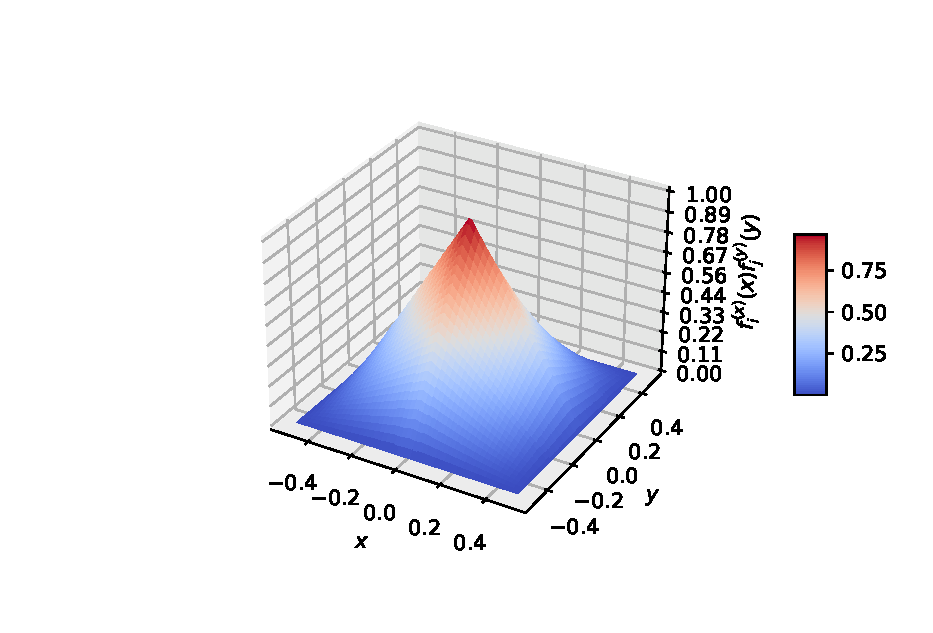
\includegraphics[width=0.8\textwidth]{./figuras/bilinearshape}
				\caption{Bilinear shape function on a rectangular grid.}
				\label{fig:3:bilinearshape}
			\end{figure}
		
			%Esta função pode representar melhor heterogeneidades nos espalhadores assim como o campo elétrico. No entanto, diferentemente da discretização por pulso,mais elementos contribuirão para o valor da função em um determinado ponto. Isso pode tornar o custo operacional da cálculo da integral \eqref{eq:3:discretization:11} mais caro, ao posso que pode melhorar a precisão da integração.
			This function can better represent heterogeneities in the scatterers as well as the electric field. However, unlike pulse discretization, more elements will contribute to the value of the function at a given point. This can make the computational cost of calculating the integral \eqref{eq:3:discretization:11} more expensive while improving integration accuracy.
			
			%Alternativamente às funções de tentativa definidas em apenas partes do domínio, existem os Métodos Espectrais no qual as funções de base são definidas em todo o domínio. A eficiência desse tipo de metodologia depende de uma escolha cuidadosa das funções, i.e., elas precisam ser uma boa representação das funções desconhecidas. IPor causa disso, esse tipo de estratégia para a discretização da função contraste pode não ser uma boa escolha. No entanto, isto pode ser compatível com a representação do campo elétrico principalmente porque, em problemas analíticos que envolvem apenas um espalhador, a solução é escrita em termos de exponenciais complexas ou funções de Bessel. Por exemplo, as funções $g^{(x)}_p(x)$ e $g^{(y)}_q(y)$ poderiam ser escolhidas de tal forma que:
			Alternatively to the trial functions defined in only pieces of the domain, the Spectral Methods define them everywhere in the domain. The efficiency of this sort of methodology depends on a careful choice of the functions, i.e., they need to be a good representation of the unknown functions. For this reason, applying such a strategy to contrast function discretization may not be a good choice, especially in the case of traditional geometries. However, this may be compatible with the representation of the electric field essentially because, in analytical problems that involve only a single scatterer, the solution is written in terms of complex exponentials or Bessel's functions. For example, the functions $g^{(x)}_p(x)$ and $g^{(y)}_q(y)$ could be chosen in such a way so that:
			\begin{align}
				g^{(x)}_p(x)g^{(y)}_q(x) = H^{(2)}_0(k_b\sqrt{(x_p-x)^2+(y_q-y)^2}) \label{eq:3:discretization:collocation:21} 
			\end{align}

			%Este exemplo de escolha remete à Colocação de Norma Mínima. Nesta abordagem, em um problema inverso linear cujo o operador $\mathcal{K} : X\rightarrow C[a,b]$ é linear, limitado e injetivo de um espaço de Hillbert $X$ em um espaço $C[a,b]$ de funções contínuas em $[a,b]$; então a função de tentativa pode ser definida como aquela cuja norma $L^2(a,b)$ é mínima. Esta solução, no caso de uma equação integral como em \eqref{eq:app:functional:4}, é o kernel $k_i(s) = k(t_i,s)$ o qual pertence a $L^2(a,b)$ \citep{kirsch2011introduction}.
			This choice example refers to the Minimum Norm Collocation. Theoretically, supposing a linear inverse problem whose operator $\mathcal{K} : X\rightarrow C[a,b]$ is linear, bounded, and injective of a space of Hillbert $X$ in a space $C[a,b]$ of continuous functions in $[a,b]$; then the trial function can be defined as the one whose norm $L^2(a,b)$ is minimum. This solution, in the case of an integral equation as in \eqref{eq:app:functional:4}, is the kernel $k_i(s) = k(t_i,s)$, which belongs to $L^2(a,b)$ \citep{kirsch2011introduction}.
			
			%De qualquer maneira, uma atenção especial sobre possíveis singularidades precisa ser tomada. Por causa disso, a descrição analítica e implementação desse tipo de método podem ser mais complexas.
			Nevertheless, exceptional attention to possible singularities needs to be taken. For this reason, the analytical description and implementation of this kind of method might be more complex.
		
		\subsection{The Galerkin Method}\label{chap:methods:discretization:galerkin}
			
			%Uma outra possilidade é escolher a função peso da mesma família das funções de tentativa, i.e.:
			Another possibility is to choose the weight function from the same family as the trial ones, i.e.:
			\begin{equation}
				w_k(x) = f_i(x) \label{eq:3:discretization:galerkin:0}
			\end{equation}
		
			%Esta estratégia é conhecida na literatura como Método do Galerkin ou Bubnov-Galerkin. Para problemas modelados a partir de equações diferenciais, a escolha dessas funções precisa atender os seguintes critérios \citep{fletcher1984computational}:
			This strategy is known in the literature as the Galerkin or Bubnov-Galerkin Method. For problems modeled from differential equations, the choice of these functions need to meet the following criteria \citep{fletcher1984computational}:
			\begin{enumerate}
				\item The weight and trial functions are chosen from the same family;
				\item Weight and trial functions must be linearly independent;
				\item The weight and trial functions must be the first N members of a dense set of functions;
				\item The weight and trial functions must satisfy the essential homogeneous boundary conditions exactly.
			\end{enumerate}
			%Enquanto a primeira condição define o método, a segunda diz respeito à relação entre equações linearmente independentes e variáveis desconhecidas. As duas últimas estão relacionadas com a eficiência do método.
			While the first condition defines the method, the second concerns the relationship between linearly independent equations and unknown variables. % The last two are related to the efficiency of the method.
		
			%No entanto, é necessário observar que, em EISP, os domínios das funções de peso e tentativa são diferentes, i.e., os argumentos das funções em \eqref{eq:3:discretization:galerkin:0} são diferentes. Além disso, é necessário integrar $E_{z_s}$ em todo o domínio $D$ \eqref{eq:3:discretization:9}. Este é um requisito que pode inviabilizar a aplicação prática do método visto que geralmente o campo espalhado só é conhecido em um conjunto finito de pontos. Uma alternativa para este problema é usar um método de interpolação. No entanto, esta estratégia pode induzir o método de inversão a soluções distantes da verdadeira.
			However, it is necessary to note that, in EISP, the domains of the weight and trial functions are different, i.e., their arguments in \eqref{eq:3:discretization:galerkin:0} are unrelated. In addition, it is necessary to integrate $E_{z_s}$ across the $D$ domain \eqref{eq:3:discretization:9}. This requirement can make the practical application of the method unfeasible since the scattered field is known only at a finite set of points. An alternative for this problem is to use an interpolation method. However, this strategy can induce the inversion to solutions far from the real one.
			
			%Por fim, podemos mencionar alguns dos poucos trabalhos na literatura que proporam metodologias baseadas nesse tipo de discretização. Ao invés de discretizarem a equação integral, \cite{zakaria2010finite} se basearam na equação da onda \eqref{eq:2:waveequations:final}. A equação diferencial foi escrita em termos do campo espalhado e da fonte de corrente. Além disto, foi imposta a condição de contorno de radiação de Sommerfield, modelada a partir de condições de absorção de segunda ordem. A partir disso, os autores utilizaram uma discretização por elementos triangulares não-uniformes e desenvolveram uma metodologia baseada na Inversão de Fonte de Contraste (a qual será explicada mais à frente no texto). Alternativamente, \cite{brown2019hybridizable} proporam uma abordagem híbrida e discontínua do Método do Galerkin para resolver o problema direto dentro do escopo da Inversão de Fonte de Contraste, a qual necessita de um número menor de graus de liberdade.
			Finally, we can mention some of the few papers in the literature that used methodologies based on this type of discretization. Rather than discretizing the integral equation, \cite{zakaria2010finite} applied it to the wave equation \eqref{eq:2:waveequations:final}. The differential equation was written in terms of the scattered field and the source. In addition, the Sommerfield radiation boundary condition was imposed, modeled with second-order absorption conditions. The authors used a non-uniform triangular elements discretization and developed a methodology based on the Contrast Source Inversion (which will be explained later in the text). Alternatively, \cite{brown2019hybridizable} proposed a hybrid and discontinuous approach to the Galerkin Method to solve the problem within the scope of the Contrast Source Inversion, which requires fewer degrees of freedom.
		
		\subsection{Some Aspects on Discretization}\label{chap:methods:discretization:aspects}
		
			%Antes de concluir a seção, dois aspectos também merecem destaque na discussão sobre discretizatição. Primeiramente, é preciso destacar que metodologias de discretização também são estratégias de regularização tal qual definido na \Autoref{chap:problemstatement:inverse} \citep{kirsch2011introduction}. A discretização é um assunto dentro do escopo de operadores de projeção. Matematicamente, um operador de projeção é definido da seguinte forma:
			Before concluding the section, two aspects also deserve to be highlighted when discussing discretization. First, it is necessary to underline that discretization methodologies are also regularization strategies, as defined in Section \ref{chap:problemstatement:inverse} \citep{kirsch2011introduction}. Discretization is an issue within the scope of projection. Mathematically, a projection operator is defined as follows:
			\vspace{1.5ex}
			\begin{definition}\label{def:3:projection}
				Projection Operator\\
				Let $X$ be a normed space over the field $\mathbb{K}=\mathbb{R}$ or $\mathbb{K}=\mathbb{C}$. Let $U\subset X$ be a closed subspace. A linear bounded operator $\mathcal{P} : X\rightarrow X$ is called a projection operator on $U$ if
				\begin{itemize}
					\item $\mathcal{P}\{x\} \in U, ~\forall x\in X$ and
					\item $\mathcal{P}\{x\} = x,~ \forall x\in U$.
				\end{itemize}
			\end{definition}
			\vspace{1.5ex}
			%Dentro deste contexto, ass funções de peso e tentativa são membras de subespaços de dimensão finita $X_n\subset X$ e $Y_n\subset Y$, respectivamente. Então, para um dado $y\in Y$ no qual $\mathcal{K}\{x\} = y$ é linear e um-pra-um, a discretização é operador de projeção $\mathcal{Q}_n : Y\rightarrow Y_n$ que resolve a equação:
			Within this context, the weight and trial functions are members of finite-dimension subspaces $X_n\subset X$ and $Y_n\subset Y$, respectively. Then, for a given $y\in Y$ in which $\mathcal{K}\{x\} = y$ is linear and one-to-one, discretization is a projection operator $\mathcal{Q}_n : Y\rightarrow Y_n$ that solves the equation:
			\begin{equation}
				\mathcal{Q}_n\left\{ K\{x_n\} \right\} = \mathcal{Q}_n\{y\} \label{eq:3:discretization:projection:0}
			\end{equation}
			
			%\noindent para $x_n\in X_n$. Então, seja $\{\hat{x}_1,\cdots,\hat{x}_n\}$ e $\{\hat{y}_1,\cdots,\hat{y}_n\}$ bases de $X_n$ e $Y_n$, respectivamente. Os termos $\mathcal{Q}_n\{y\}$ e $\mathcal{Q}_n\left\{ K\{x_n\}\right\}$ pode ser representados na seguinte forma:
			\noindent for $x_n\in X_n$. So, let $\{\hat{x}_1,\cdots,\hat{x}_n\}$ and $\{\hat{y}_1,\cdots,\hat{y}_n\}$ be bases of $X_n$ and $Y_n$, respectively. The terms $\mathcal{Q}_n\{y\}$ and  $\mathcal{Q}_n\left\{ K\{x_n\}\right\}$ can be represented as follows:
			\begin{align}
				\mathcal{Q}_n\{y\} &= \sum\limits_{i=1}^n b_i\hat{y}_i, ~~~~j=1,\cdots,n \label{eq:3:discretization:projection:1} \\
				\mathcal{Q}_n\left\{ K\{x_n\}\right\} &= \sum\limits_{i=1}^n A_{ij}\hat{y}_i, ~~j=1,\cdots,n \label{eq:3:discretization:projection:2}
			\end{align}
		
			%\noindent no qual $b_{i}$, $A_{ij}\in\mathbb{K}$. A combinação linear $x_n = \sum_{j=1}^n a_j\hat{x}_j$ é solução de \eqref{eq:3:discretization:projection:0} se e somente se $\{a_1,\cdots,a_n\} \in \mathbb{K}^n$ é solução do sistema finito de equações lineares:
			\noindent in which $b_{i}$, $A_{ij}\in\mathbb{K}$. The linear combination $x_n = \sum_{j=1}^n a_j\hat{x}_j$ is a solution of \eqref{eq:3:discretization:projection:0} if and only if $\{a_1,\cdots,a_n\} \in \mathbb{K}^n$ is a solution of the finite system of linear equations:
			\begin{equation}
				\sum\limits_{i=1}^n A_{ij} a_j = b_i, ~~ i=1,\cdots,n \label{eq:3:discretization:projection:3}
			\end{equation}
			
			%Neste contexto, o Método da Colocação é um exemplo de método de projeção cujo operador é denominado operador de interpolação. Já o Método do Galerkin é conhecido como um operador de projeção ortogonal.
			In this context, the Collocation Method is an example of a projection method whose operator is called an interpolation one. The Galerkin Method is known as an orthogonal projection operator. This implies that the error is orthogonal to the approximation space and the solution is the best one (minimum error) in that approximation space.
			
			%Em segundo lugar, a escolha do tamanho do conjunto de funções de peso e de tentativa ($N_U$, $N_V$, $N_I$, $N_J$, $N_P$, $N_Q$ e $N_S$) precisam levar em conta não só os aspectos discutidos sobre graus de liberdade na \Autoref{chap:problemstatement:eisp:5} mas também um conceito conhecido na literatura como Crime Inverso. Como destacou \cite{colton2019inverse}, é necessário que, quando a experimentação de métodos para EISP envolver dados sintéticos gerados por resolvedores diretos, este último não deve ter conexões com o resolvedor inverso. Em outras palavras, em um problema inverso de dimensão finita, é necessário evitar soluções triviais.
			Second, the choice of trial functions, i.e., its shape and size, needs to consider not only the aspects discussed about degrees of freedom in Subsection \ref{chap:problemstatement:eisp:5} but also a concept in the literature known as Inverse Crime. As highlighted by \cite{colton2019inverse}, it is necessary that, when the experimentation involves synthetic data generated by direct solvers, the latter must not have connections with the inverse solver. In other words, in an inverse problem of finite dimension, trivial solutions should be avoided.
			
			%O conceito pode ser exemplificado através de um problema genérico onde é o objetivo é recuperar uma família $G_m$ de superfícies de contorno com $m$ parâmetros. Se, para este problema, utilizarmos dados sintetizados por um resolvedor direto \textbf{M} para obter $n$ dados de entrada, como por exemplo, amostras de campo distante. Isto equivale a uma função $g : \mathbb{R}^m \rightarrow \mathbb{C}^n$. Portanto, se uma determinada superfície $\partial D\in G_m$ é gerada a partir do conjunto de parâmetros $a_0$, um método de inversão que incorpora o mesmo resolvedor direto \textbf{M} não está fazendo nada mais do que resolver o problema de dimensão finita $g(a) = g(a_0)$. Por isso, a superfície $\partial D$ será inevitavelmente bem reconstruída, pressupondo que $m$ e $n$ não são grandes demais.
			The concept can be illustrated through a generic problem where its objective is to recover a family $G_m$ of contour surfaces with $m$ parameters. For this problem, if we use data synthesized by a direct resolver \textbf{M} to obtain $n$ input data, such as distant field samples, this is equivalent to a function $g : \mathbb{R}^m \rightarrow \mathbb{C}^n$. Therefore, if a given surface $\partial D\in G_m$ is generated from the set of parameters $p_0$, an inversion method that incorporates the same direct solver \textbf{M} is doing nothing more than solving the finite dimension problem $g(p) = g(p_0)$. Therefore, the $\partial D$ surface will inevitably be well reconstructed, assuming that $m$ and $n$ are not too big.
			
			%\cite{wirgin2004inverse} trouxe mais contribuições para o assunto através da análise de três exemplos os quais, mesmo não sendo universais, aprofundaram o entendimento sobre o conceito introduzido por \cite{colton2019inverse}. As conclusões feitas por Wirgin podem ser resumidas em:
			\cite{wirgin2004inverse} brought more contributions to the subject by analyzing three examples that, although not universal, deepened the understanding of the concept introduced by \cite{colton2019inverse}. The conclusions made by Wirgin can be summarized in:
			\begin{itemize}
				\item Regarding the meaning of the lack of connection between a direct solver and an inverse one, he proposed that its practical meaning is the difference in the number of terms of the power series representing the forward and inverse solver. That is, if that number of terms are different, then there would be no connection.
				%\item Wirgin concluiu que quanto maior a diferença entre ambas as partes em termos de seus funcionais, maior o erro relativo da inversão. Isso significa que reconstruir os parâmetros com muita precisão são é possível quando os dois resolvedores têm conexão.
				\item Wirgin concluded that the more significant difference between both solvers in terms of their functionals, the larger relative inversion error. That means recovering the parameters very accurately is possible when the two resolvers are connected.
				%\item Cometer o crime inverso também tem o sentido prático de pelo menos revelar se o problema inverso tem ou não solução única.
				\item Committing the inverse crime also has the practical sense of at least revealing whether the inverse problem has a unique solution or not.
				%\item Quando o crime inverso é cometido, a solução pode não ser somente a ``solução trivial'', mas também podem ser observadas outras por meio de um método numérico robusto, as quais não necessariamente seriam observadas numa situação onde o crime não é cometido. 
				\item When the inverse crime is committed, the solution may not only be the ``trivial'' one, but others can also be observed through a robust numerical method system, which would not necessarily be observed in a situation where the crime is not committed.
			\end{itemize}
		
			%Wirgin também critica o uso do termo ``solução trivial'' para o assunto uma vez que o objetivo é de fato reconstruir os parâmetros com maior precisão possível. Além disso, mesmo que sua análise matemática se baseie na reconstrução de um único parâmetro por um único dado, a análise matemática para problema maiores, inclusive dois parâmetros e dois dados, se torna muito mais complicada. No entanto, ele afirma que seria difícil de esperar contradições entre suas conclusões para um caso mais simples e as que porventura poderiam ser obtidas para casos mais complexos. Por fim, em experimentos com dados reais não faz sentido a preocupação com o crime inverso uma vez que, na verdade, o ``resolvedor direto'' é desconhecido. Mesmo que um resolvedor direto represente mimetize bem o fenômeno físico, isso não impede que se observe perturbações na solução que representem algo falso.
			Wirgin also criticizes the use of the term ``trivial solution'' since the objective is, in fact, to recover the parameters as accurately as possible. In addition, even if his mathematical analysis is based on the reconstruction of a single parameter for a single data, mathematical analysis for larger problems, including two parameters and two data, becomes much more complicated. However, he claims that it would be difficult to expect contradictions between their conclusions for a simple case and those that might be obtained for more complex ones. Finally, in experiments with real data, it does not make sense to worry about inverse crime since, in fact, the ``direct resolver'' is unknown. Even that a direct solver represents the physical phenomenon well, this does not prevent the observation of disturbances in the solution, representing something false.
		
	\section{The Linear Case}\label{chap:methods:linear}
			
		%Embora EISP seja não-linear, o estudo do caso linear é muito importante pelo motivo que muitos métodos utilizam estratégias de linearização do problema. Estas estratégias podem ser importantes tanto para definir direções de busca como para definir soluções iniciais. Além disso, é possível utilizar aproximações para o campo total para problemas que pressupõem espalhadores fracos. Neste caso, o problema se torna linear. Isto possibilita a utilização das metodologias clássicas de regularização de operadores lineares compactos e limitados. A discretização de \eqref{eq:3:discretization:collocation:3} e \eqref{eq:3:discretization:10} serão utilizadas para discutir as metodologias traditionais. No entanto, todas essas metodologias podem ser facilmente adaptadas para as outras equações e discretizações.
		%Although EISP is non-linear, the study of the linear case is significant because many methods use strategies based on problem linearization. These strategies can be essential when defining search directions and initial solutions. In addition, it is possible to use approximations for the total field in problems where we assume weak scatterers. In this case, the problem may be approximated to a linear one. This approximation enables the use of traditional regularization methodologies for compact and bounded linear operators. The discretization of \eqref{eq:3:discretization:collocation:3} and \eqref{eq:3:discretization:10} will be used to discuss them. However, all of these methodologies can be easily adapted to other equations and discretizations.
		Although EISP is non-linear, the study of the linear case is significant because many methods use strategies based on problem linearization. These strategies can be essential when defining search directions and initial solutions. In addition, it is possible to use approximations for the total field in problems where we assume weak scatterers. In this case, the problem may be approximated to a linear one. The discretization of \eqref{eq:3:discretization:collocation:3} and \eqref{eq:3:discretization:10} will be used to discuss them. However, all of these methodologies can be easily adapted to other equations and discretizations.
			
		\subsection{Approximated Solutions for Weak Scatterers}\label{chap:methods:linear:weak}
				
			%Quando as propriedades dielétricas de um espalhador diferem muito pouco do meio de fundo, ele é considerado um espalhador fraco. Nestas condições, é possível fazer aproximações em relação ao campo elétrico e tornar o problema linear. Existem duas técnicas clássicas que abordam esta situação: a Aproximação de Born (BA) e a Aproximação de Rytov (RA). A primeira é mais adequada para baixas frequências enquanto que a segunda é mais adequada para altas.
			When the dielectric properties of a scatterer differ very little from the background, and its size is not too large, it is considered a weak one (DNL $\ll1$). Under these conditions, it is possible to approximate the electric field and turn the problem into a linear one. Two classic techniques address this situation: the Born Approximation (BA) and the Rytov Approximation (RA). The first is best suited for low frequencies, while the second is more suitable for high ones.
			
			%A série de Born é uma metodologia a qual escreve o campo elétrico como uma série em termos da função de Green, do contraste e do campo incidente. Se a norma $L^2(S)$ na qual $||\int_S d\mathbf{r^\prime} \mathbf{\bar{G}}(\mathbf{r},\mathbf{r^\prime})\chi(\mathbf{\mathbf{r^\prime}})||<1$, então:
			Born's series is a methodology that writes the electric field as a series in terms of Green's function, contrast, and incident field. Recapitulating the formulas from Subsection \ref{chap:problemstatement:eisp:4}, if the $L^2(S)$-norm $$\left\|\int_S d\mathbf{r^\prime} \mathbf{\bar{G}}(\mathbf{r},\mathbf{r^\prime})\chi(\mathbf{\mathbf{r^\prime}})\right\|<1,$$ then:
			\begin{equation}
				\mathbf{E}(\mathbf{r}) = \sum\limits_{n=0}^\infty \left(\int_Sd\mathbf{r^\prime} \mathbf{\bar{G}}(\mathbf{r},\mathbf{r^\prime})\chi(\mathbf{r^\prime})\right)^n\mathbf{E}_i(\mathbf{r}) \label{eq:3:linear:bornseries:analytic}
			\end{equation}
			
			%Seguindo a forma matricial \eqref{eq:3:discretization:collocation:11}, \eqref{eq:3:linear:bornseries:analytic} pode ser escrita de maneira discretizada como:
			Following the matrix form \eqref{eq:3:discretization:collocation:11}, \eqref{eq:3:linear:bornseries:analytic} can be written in a discretized fashion as:
			\begin{equation}
				\mathbf{\bar{E}} = \sum\limits_{n=0}^\infty (\mathbf{\bar{G}^S}\boldsymbol{\bar{\chi}})^n\mathbf{\bar{E}^i} \label{eq:3:linear:bornseries:discrete}
			\end{equation}
			
			%A Aproximação de Born de Primeira-Ordem é uma single-scattering approximation obtida a partir da truncamento da série de Born \eqref{eq:3:linear:bornseries:analytic} em seu primeiro termo $n=0$, i.e.:
			The First-Order Born Approximation is a single-scattering approximation obtained from the truncation of the Born series \eqref{eq:3:linear:bornseries:analytic} in its first term $n = 0$, i.e.:
			\begin{equation}
				\mathbf{E}(\mathbf{r}) \approx \mathbf{E}_i(\mathbf{r}) \label{eq:3:linear:bornapproximation}
			\end{equation}		
			
			%Convém destacar que \eqref{eq:3:linear:bornapproximation} é também equivalente a uma aproximação de primeira-ordem da expansão em séries de Neumman da equação integral \eqref{eq:2:eisp:2} e a uma aproximação por séries de Taylor de $\mathbf{E}(\mathbf{r})$ \citep{chew1995}.
			
			%Embora ela até viole o princípio de conservação de energia, o teorema da reciprocidade é ainda válido por causa da simetria da função diádica de Green \citep{chew1995}. Além disso, se o tamanho do espalhador é da ordem $L$ no qual $k_bL \ll 1$, então a função diádica de Green \eqref{eq:app:green:17}, o contraste e a integral volumétrica podem ser aproximadas por \citep{chew1995}:
			Although it even violates the energy conservation principle, the reciprocity is still valid because of the symmetry of dyadic Green's function \citep{chew1995}. In addition, if the size of the scatterer is of the order $L$ in which $k_bL \ll 1$, then dyadic Green's function \eqref{eq:app:green:17}, contrast and volumetric integral can be approximated by \citep{chew1995}:
			\begin{align}
				\mathbf{\bar{G}}(\mathbf{r},\mathbf{r^\prime}) &\approx \left(1+\frac{1}{k_b^2L^2}\right)\frac{1}{L} \label{eq:3:linear:bornapproximation:1} \\
				k^2(\mathbf{r})-k_b^2 &\approx k_b^2\Delta\epsilon_r \label{eq:3:linear:bornapproximation:2} \\
				\int_D d\mathbf{r^\prime} &\approx L^3 \label{eq:3:linear:bornapproximation:3}
			\end{align}
			
			%\noindent onde $\Delta\epsilon_r = \epsilon_r/\epsilon_{rb} - 1$. Desta forma, \eqref{eq:2:eisp:2} é aproximada por:
			\noindent where $\Delta\epsilon_r = \epsilon_r/\epsilon_{rb} - 1$. Thus, \eqref{eq:2:eisp:2} is approximated by:
			\begin{equation}
				\mathbf{E}_s(\mathbf{r}) \approx \left[(k_bL)^2+1\right]\Delta\epsilon_r\mathbf{E}_i(\mathbf{r}) \label{eq:3:linear:bornapproximation:4}
			\end{equation}
		
			%No entanto, em situações onde a frequência é mais alta, a variação do campo dentro do objeto é preponderante. Nestes casos, o operador $\nabla\nabla$ é aproximado por $k_b^2$ e a fase do campo dentro do espalhador precisa ser levada em conta. Pressupondo que o campo dentro do espalhador é uma superposição de ondas planas, a aproximação de \eqref{eq:3:linear:bornapproximation} precisa ser corrigida para:
			However, in situations where the frequency is higher, the field variation inside the object is dominant. In these cases, the operator $\nabla\nabla$ is approximated by $k_b^2$ and the field phase within the scatterer needs to be taken into account. Assuming that the field inside the scatterer is a superposition of plane waves, the approximation in \eqref{eq:3:linear:bornapproximation} needs to be fixed to:
			\begin{equation}
				\mathbf{E}(\mathbf{r}) \approx \mathbf{E}_i(\mathbf{r})e^{j(\mathbf{k}-\mathbf{k_b})\cdot\mathbf{r}}  \label{eq:3:linear:bornapproximation:5}
			\end{equation}
		
			%Esta aproximação depende que $(k-k_b)L\ll1$, a qual é uma restrição mais forte que a anterior.
			This approximation depends on $(k-k_b)L\ll1$, which is a stronger constraint than the previous one.
			
			%A Aproximação de Primeira-Ordem de Rytov é baseada numa redução da equação vetorial por uma equação escalar. Esta redução consiste na substituição do campo total por uma exponencial complexa cuja fase é função, i.e.:
			Rytov's First-Order Approximation is based on a reduction in the vector equation by a scalar equation. This reduction consists of replacing the total field by a complex exponential whose phase is a function, i.e.:
			\begin{equation}
				E_z(\mathbf{r}) \approx E_{i_z}(\mathbf{r})^{\psi(\mathbf{r})} \label{eq:3:linear:rytov:0}
			\end{equation}
		
			%\noindent no qual a fase de primeira-ordem $\psi(\mathbf{r})$ é baseada no campo espalhado de \eqref{eq:2:eisp:2} calculado pela Aproximação de Born \eqref{eq:3:linear:bornapproximation}, i.e.:
			\noindent in which the first-order phase $\psi(\mathbf{r})$ is based on the scattered field of \eqref{eq:2:eisp:2} calculated by the Born Approximation \eqref{eq:3:linear:bornapproximation}, i.e.:
			\begin{equation}
				\psi(\mathbf{r}) = \frac{1}{E_i(\mathbf{r})} \int_S d\mathbf{r^\prime} g(\mathbf{r},\mathbf{r^\prime})E_{i_z}(\mathbf{r^\prime})\chi(\mathbf{r^\prime}) \label{eq:3:linear:rytov:1}
			\end{equation}
		
			%Aplicando uma análise semelhante a \eqref{eq:3:linear:bornapproximation:1}-\eqref{eq:3:linear:bornapproximation:3}, é possível demonstrar que $\psi(\mathbf{r}) \approx k_b^2L^2\Delta\epsilon_r$ quando $k_bL\rightarrow0$ \citep{chew1995}. Esta condição é equivalente a $(k_bL)^2\Delta\epsilon_r\ll1$. Por outro lado, se a frequência tende ao infinito, então $\psi(\mathbf{r}) \approx k_bL\Delta\epsilon_r$. A condição para esta aproximação é $\Delta\epsilon_r \ll 1$, a qual é muito mais fraca que a anterior. Por isso, esta aproximação é mais adequada para altas frequências.
			When we apply an analysis similar to \eqref{eq:3:linear:bornapproximation:1}-\eqref{eq:3:linear:bornapproximation:3}, it is possible to demonstrate that $\psi(\mathbf{r}) \approx k_b^2L^2\Delta\epsilon_r$ when $k_bL\rightarrow0$ \citep{chew1995}. This condition is equivalent to $(k_bL)^2\Delta\epsilon_r\ll1$. On the other hand, if the frequency tends to infinity, then $\psi(\mathbf{r}) \approx k_bL\Delta\epsilon_r$. The condition for this approximation is $\Delta\epsilon_r \ll 1$, which is much weaker than the previous one. Therefore, this approach is more suitable for high frequencies.
		
		\subsection{The Back-Propagation Method}\label{chap:methods:linear:backpropagation}
		
			The Back-Propagation (BP) Method is noniterative algorithm which is able to provide a solution for the contrast image. Such solution is often used as initial guess in many methods. The method is suitable for arbitrary incident fields, near and far fields measurements. BP is based on three steps: (i) estimate the induced current; (ii) compute total field in $S$ through the state equation; and (iii) determine the contrast image by relation between total field and induced current. If the induced current is assumed to be proportional to the back-propagation field, then the induced current is evaluated according to:
			\begin{equation}
				\mathbf{\bar{J}^{eq}} = \gamma \mathbf{\bar{G}^{D*}} \mathbf{\bar{E}^s} \label{eq:3:linear:bp:J}
			\end{equation}
		
			\noindent where the superscript $\mathbf{^*}$ is the operator's adjoint and numerically given by the conjugated-transposed. The parameter $\gamma$ is a complex value that is chosen to minimize the cost function defined as the quadratic error in the scattered field:
			\begin{equation}
				F(\gamma) = ||\mathbf{\bar{E}^s} - \mathbf{\bar{G}^D}(\gamma\mathbf{\bar{G}^{D*}}\mathbf{\bar{E}^s})||^2 \label{eq:3:linear:bp:F}
			\end{equation}
		
			The minimum of \eqref{eq:3:linear:bp:F} might be obtained analytically and is given as follows:
			\begin{equation}
				\gamma = \frac{\langle \mathbf{\bar{E}^s}, \mathbf{\bar{G}^D}\mathbf{\bar{G}^{D*}}\mathbf{\bar{E}^s}\rangle}{||\mathbf{\bar{G}^D}\mathbf{\bar{G}^{D*}}\mathbf{\bar{E}^s}||}
			\end{equation}

			\noindent where $\langle\cdot,\cdot\rangle$ is the inner product, which is numerically computed as the product between the transpose of the first argument and the complex conjugate of the second one.
			
			Once the induced current is obtained, then the total electric field might be evaluated according to \eqref{eq:3:discretization:collocation:11} replacing $\boldsymbol{\bar{\chi}}\mathbf{\bar{E}}$ by $\mathbf{\bar{J}^{eq}}$. Finally, the contrast might be evaluated according to:
			\begin{equation}
				\chi_{ij} = \frac{\sum\limits_{s=1}^{N_S}J^{eq}_{ijs}E^*_{ijs}}{\sum\limits_{s=1}^{N_S}|E^*_{ijs}|^2} \label{eq:3:linear:bp:x}
			\end{equation}
		
			If it is known that only lossless scatterers are present, then the imaginary part of $\boldsymbol{\bar{\chi}}$ can be neglected.
			
		\subsection{Dominant Current Scheme}\label{chap:methods:linear:dominantcurrent}
			
			In nonlinear problems with large number of variables, there may be some unknowns which are more relevant. Since recovering the induced current might be a hard task when a limited number of measurements are available, the dominant part of the induced current might be prioritized. Such strategy is based on the fact that the dominant current contains the most important features of the unknown scatterers and it is more robust against noise. This is the core idea behind the Dominant Current Scheme (DCS) \citep{wei2019deep}.
			
			When the Singular Value Decomposition is applied to $\mathbf{\bar{G}^D}$, the dominant current might be evaluated according to:
			\begin{equation}
				\mathbf{\bar{J}^{eq}}_+ = \sum\limits_{n=1}^L \frac{\bar{u}^*_n\cdot \mathbf{\bar{E}}^s}{\xi_n}\bar{v}_j \label{eq:3:linear:dcs:j+}
			\end{equation}
		
			\noindent where $\bar{u}$, $\bar{v}$, and $\xi$ are the left, right, and singular value vectors from the decomposition; and $L$ is an index that limits the singular values in descending order, i.e., the dominant current is computed taking into account the first $L$ largest singular values. Therefore, the $N_IN_J - L$ smallest singular values are neglected and unstable components corrupted by noise are avoided. However, a compensation for the missing information is also provided, i.e.:
			\begin{equation}
				\mathbf{\bar{J}^{eq}}_- = \mathbf{\bar{F}}\cdot\boldsymbol{\alpha} \label{eq:3:linear:dcs:j-}
			\end{equation}
		
			\noindent where $\mathbf{\bar{F}}$ and $\boldsymbol{\alpha}$ are the low-frequency matrices composed by the first $m$ low-frequency  Fourier bases and their corresponding coefficients, respectively. Since $\boldsymbol{\alpha}$ is an unknown, some approximation has to be made to complete the scheme. \cite{wei2019deep} proposed the following objective-function:
			\begin{equation}
				F(\boldsymbol{\alpha}) = \left[ \frac{||\mathbf{\bar{G}^F}\cdot\boldsymbol{\alpha}+\mathbf{\bar{G}^E}||^2}{||\mathbf{\bar{E}^s}||^2}+\frac{||\mathbf{\bar{A}}\cdot\boldsymbol{\alpha}+\mathbf{\bar{B}}||^2    }{||\mathbf{\bar{J}^{eq}_+}||^2}\right] \label{eq:3:linear:dcs:f}
			\end{equation}
		
			\noindent where $\mathbf{\bar{G}^F} = \mathbf{\bar{G}^D}\cdot\mathbf{\bar{F}}$, $\mathbf{\bar{G}^E} = \mathbf{\bar{G}^D}\cdot\mathbf{\bar{J}^{eq}}_+ - \mathbf{\bar{E}^s}$, $\mathbf{\bar{A}} = \mathbf{\bar{F}} -\boldsymbol{\bar{\chi}}\cdot\mathbf{\bar{G}^s}\cdot\mathbf{\bar{F}}$, and $\mathbf{\bar{B}} = \boldsymbol{\bar{\chi}}(\mathbf{\bar{E}^i}+\mathbf{\bar{G}^S}\mathbf{J^{eq}}_+)-\mathbf{J^{eq}_-}$.
			
			Based on \eqref{eq:3:linear:dcs:f}, the authors proposed an iterative process to update $\boldsymbol{\bar{\chi}}$ and $\boldsymbol{\alpha}$, starting by $\boldsymbol{\bar{\chi}}=\mathbf{0}$. The variable $\boldsymbol{\alpha}$ is approximated according to $\boldsymbol{\alpha} = \beta\boldsymbol{\gamma}$ where:
			\begin{eqnarray}
				\boldsymbol{\gamma} &=& \left( \frac{\mathbf{\bar{G}^{F*}}\cdot\mathbf{\bar{G}^E}}{||\mathbf{\bar{E}^s}||^2}-\frac{\mathbf{\bar{A}^{*}}\cdot\mathbf{\bar{B}}}{||\mathbf{\bar{J}^{eq}}||^2}\right) \label{eq:3:linear:dcs:rho} \\
				\beta &=& \frac{Num}{Den} \\
				Num &=& -\frac{\mathbf{\bar{G}^{F*}}\cdot\boldsymbol{\gamma}\cdot\mathbf{\bar{G}^E}}{||\mathbf{\bar{E}^s}||^2} + \frac{(\mathbf{\bar{A}}\cdot\boldsymbol{\gamma})^{*}\cdot\mathbf{\bar{B}}}{||\mathbf{\bar{J}^{eq}_+}||^2} \\
				Den &=& \frac{||\mathbf{\bar{G}^{F}}\cdot\boldsymbol{\gamma}||^2}{||\mathbf{\bar{E}^s}||^2} + \frac{||\mathbf{\bar{A}}\cdot\boldsymbol{\gamma}||^2}{||\mathbf{\bar{J}^{eq}_+}||^2}
			\end{eqnarray}
		
			Then, after using $\boldsymbol{\alpha}$ to compute the low-frequency compensation through \eqref{eq:3:linear:dcs:j-}, the following steps are required:
			\begin{eqnarray}
				\mathbf{\bar{J}^{eq}} &=& \mathbf{\bar{J}^{eq}_+} + \mathbf{\bar{J}^{eq}_-} \\
				\mathbf{\bar{E}} &=& \mathbf{\bar{E}^i} + \mathbf{\bar{G}^S}\mathbf{\bar{J}^{eq}} \\
				\chi_{ijs} &=& \frac{J^{eq}_{ijs}E_{ijs}^*}{||E_{ijs}||^2} \label{eq:3:linear:dcs:x}
			\end{eqnarray}
		
			In \eqref{eq:3:linear:dcs:x}, it is computed one contrast image for each incidence. The authors had decided for this based in its application to Convolution Neural Networks. However, a computation similar to \eqref{eq:3:linear:bp:x} might also be used.

	\section{Regularization Methods}\label{chap:methods:regularization}
	
		Whenever the total electric field in the state space is known, the inverse problem turns into a linear one. This may happen when approximating the total field by the incident one (subsection \ref{chap:methods:linear:weak}) or when a forward solver is employed to determine it for a given outdated contrast image. For a linear problem, regularization methods might be applied to solve an inverse problem which usually has more unknowns than equations. In the next subsections, traditional regularization methods will be covered.

		\subsection{The Tikhonov Regularization}\label{chap:methods:linear:tikhonov}
			
			%Talvez a mais conhecida técnica de regularização de problemas inversos com operadores lineares e limitado é a Regularização de Tikhonov \citep{tikhonov1963regularization,kirsch2011introduction}. Não somente nesse caso como também em sistemas de equações lineares superdeterminados, i.e., onde o número de equações é menor que o de variáveis. De um modo geral, o princípio deste método é determinar a solução $x\in X$ que minimiza $||\mathcal{K}\{x\} = y||$ para alguma norma em $Y$. Se $X$ tem dimensão finita e $\mathcal{K}$ é compacto, o problema de minimização também é mal-posto.
			Perhaps the most traditional technique for regularizing inverse problems with linear and limited operators is the Tikhonov Regularization \citep{tikhonov1963regularization,kirsch2011introduction}. Not only in this case but also in underdetermined systems of equations, i.e., where the number of equations is less than that of variables. In general, the principle of this method is to determine the solution $x\in X$ that minimizes $||\mathcal{K}\{x\} = y||$ for some norm in $Y$. If $X$ has a finite dimension and $\mathcal{K}$ is compact, then the minimization problem is also ill-posed.
			
			%A Regularização de Tikhonov propõe determinar uma solução $x^\alpha\in X$ a qual minimiza o funcional de Tikhonov $J_\alpha$:
			The Tikhonov Regularization proposes to determine a solution $x^{\alpha_T}\in X$ which minimizes the Tikhonov's functional $J_{\alpha_T}$\footnote{Another possible interpretation for the Tikhonov Regularization was recently proposed by \cite{gerth2021new}. The author has observed that the exact solution is estimated from the range of the adjoint operator and the properties are derived through the concept of approximate source conditions.}:
			\begin{equation}
				J_{\alpha_T}(x) \coloneqq ||\mathcal{K}\{x\}-y||^2 + \alpha_{T}||x||^2 \label{eq:3:linear:tikhonov:functional}
			\end{equation}

			%\noindent no $\alpha_{T} > 0$ é uma constante e $X$ e $Y$ são espaços de Hilbert. Nesse caso, $x^\alpha$ é solução de:
			\noindent in which $\alpha_{T} > 0$ is a constant and $X$ and $Y$ are Hilbert spaces. In this case, $x^{\alpha_T}$ is the solution of:
			\begin{equation}
				\alpha_Tx^{\alpha_T} + \mathcal{K}^*\{\mathcal{K}\{x^\alpha\}\} = \mathcal{K}^*\{y\} \label{eq:3:linear:tikhonov:equation}
			\end{equation}
		
			%\noindent onde $\mathcal{K}^*$ é o operador adjunto de $\mathcal{K}$. Portanto, a solução $x^\alpha$ pode ser escrita na forma de \eqref{eq:2:inverse:2} através:
			\noindent where $\mathcal{K}^*$ is the adjoint operator of $\mathcal{K}$. Therefore, the solution $x^{\alpha_T}$ can be written in the form in \eqref{eq:2:inverse:2} through
			\begin{equation}
				\mathcal{R}_{\alpha_T} \coloneqq \left(\alpha_T\mathcal{I} + \mathcal{K}^*\mathcal{K}\right)^{-1}\mathcal{K}^* : Y \rightarrow X \label{eq:3:linear:tikhonov:operator}
			\end{equation}
			
			%\noindent onde $\mathcal{I}$ é o operador identidade. O sistema linear \eqref{eq:3:linear:tikhonov:equation} também pode ser escrito como:
			\noindent where $\mathcal{I}$ is the identity operator. The linear system \eqref{eq:3:linear:tikhonov:equation} can also be written as:
			\begin{equation}
				\left(\alpha_T\mathcal{I} + \mathcal{K}^*\mathcal{K}\right)x^{\alpha_T} = \mathcal{K}^*\{y\} \label{eq:3:linear:tikhonov:linearsystem}
			\end{equation}
		
			%O limite superior do erro para essa aproximação é conhecido e expresso em termos da norma do erro em $y$, i.e., $||y-y^\delta||\le\delta$; e em termos de uma constante $E$ tal que $||z||\le E$ e $x=\mathcal{K}^*\{z\}\in\mathcal{K}^*\{Y\}$. Neste caso, se $\alpha_T(\delta) = c\delta/E$ para um $c>0$, então \citep{kirsch2011introduction}:
			The upper limit of the error for this approximation is known and expressed in terms of the norm of error in $y$, i.e., $||y-y^\delta||\le\delta$; and in terms of a constant $\Delta$ such that $||z||\le\Delta$, $x=\mathcal{K}^*\{z\}\in\mathcal{K}^*\{Y\}$, and $z\in Y$. In this case, if $\alpha_T(\delta) = c\delta/\Delta$ for a $c>0$, then the error of the solution $x^{\alpha_T(\delta),\delta}$, which is based on these assumptions, follows below \citep{kirsch2011introduction}:
			\begin{equation}
				||x^{\alpha_T(\delta),\delta}-x|| \le \frac{1}{2}\left(1/\sqrt{c}+\sqrt{c}\right)\sqrt{\delta E} \label{eq:3:linear:tikhonov:error:1}
			\end{equation}
		
			%Por um outro lado, se a função auxiliar $z$ é definida como $x=\mathcal{K}\{\mathcal{K}^*\{z\}\}\in\mathcal{K}\{\mathcal{K}^*\{X\}\}$ e a escolha $\alpha_{T}(\delta) = c(\delta/E)^{2/3}$ para um $c>0$, então o limite superior do erro será \citep{kirsch2011introduction}:
			On the other hand, if the auxiliary function $z$ is defined as$x=\mathcal{K}\{\mathcal{K}^*\{z\}\}\in\mathcal{K}\{\mathcal{K}^*\{X\}\}$ and choosing $\alpha_{T}(\delta) = c(\delta/\Delta)^{2/3}$ for a $c>0$, then the upper limit of the error it will be \citep{kirsch2011introduction}:
			\begin{equation}
				||x^{\alpha_T(\delta),\delta}-x|| \le \left(\frac{1}{2\sqrt{c}}+c\right)\Delta^{1/3}\delta^{2/3} \label{eq:3:linear:tikhonov:error:2}
			\end{equation}
		
			%Em outras palavras, \eqref{eq:3:linear:tikhonov:error:1} e \eqref{eq:3:linear:tikhonov:error:2} estabelecem que a regularização de Tikhonov é ótima dada informação $||\left(\mathcal{K}^*\right)^{-1}\{x\}||\le E$ ou $||\left(\mathcal{K}^*\mathcal{K}\right)^{-1}\{x\}||\le E$, desde que $\mathcal{K}^*$ seja um-pra-um.
			In other words, \eqref{eq:3:linear:tikhonov:error:1} and \eqref{eq:3:linear:tikhonov:error:2} establish that Tikhonov regularization is optimum given information $||\left(\mathcal{K}^*\right)^{-1}\{x\}||\le \Delta$  or $||\left(\mathcal{K}^*\mathcal{K}\right)^{-1}\{x\}||\le \Delta$, provided that $\mathcal{K}^*$ is an one-to-one operator.
			
			%Vale à pena destacar que, de uma forma prática, o método de regularização corrige os autovalores do sistema. Em outras palavras, se os autovalores de $\mathcal{K}$ tendem a zero devido a sua má-posição, os de $\alpha_{T}\mathcal{I} + \mathcal{K}^*\mathcal{K}$ são estabelecidos acima de zero por $\alpha_T>0$. Destaca-se também a relação entre a escolha de $\alpha_T$ e $\delta$. Esta relação é tal que $\alpha_T$ tende a zero quando $\delta\rightarrow0$. No entanto a velocidade de convergência não chega a ser da ordem de $\delta^2$. Além disso, quanto mais suave $x$ é, mais devagar $\alpha_T$ tenderá a zero. Portanto, em situações onde já é conhecido que a suavidade é um aspeto predominante da solução $x$, o método de regularização de Tikhonov não é ótimo. Nestes casos, os métodos de Landweber e do Gradiente-Conjugado, os quais serão discutidos em breve, têm melhor desempenho.
			It is worth noting that the regularization method is also a correction to the eigenvalues of the system. In other words, if the eigenvalues of $\mathcal{K}$ tend to zero due to their ill-posedness, those of $\alpha_{T}\mathcal{I} + \mathcal{K}^*\mathcal{K}$ are established above zero by $\alpha_T>0$. Also highlighted is the relationship between the choice of $\alpha_T$ and $\delta$. This relationship is such that $\alpha_T$ tends to zero when $\delta\rightarrow0$. Also, the smoother $x$ is, the slower $\alpha_T$ will tend to zero. Therefore, in situations where it is already known that smoothness is a predominant aspect of solution $x$, the Tikhonov regularization method is not optimal. In these cases, the Landweber and Gradient-Conjugate methods, which will be discussed soon, perform better.
			
			%O método pode ser aplicado na equação matricial \eqref{eq:3:discretization:collocation:10}. Para isso, é necessário definir o vetor-coluna $\boldsymbol{\chi}$ o qual representa a diagonal principal de $\boldsymbol{\bar{\chi}}$ e o vetor-coluna $\mathbf{\bar{E}}^{\mathbf{s}F}$\footnote{No restante do texto, o operador ``$^F$'' sempre será utilizado com o significado de transformação de matriz em vetor-coluna. A ordem será padronizada em coluna primeiro e linha depois. A letra $F$ foi escolhida com objetivo de remeter à palavra \textit{flatten}.} o qual é o rearranjo da matriz $\mathbf{\bar{E}^s}$ na seguinte forma:
			The method can be applied to the matrix equation \eqref{eq:3:discretization:collocation:10}. This is achieved if we define the column vector $\boldsymbol{\chi}$, which represents the main diagonal of $\boldsymbol{\bar{\chi}}$ and the column vector $\mathbf{\bar{E}}^{\mathbf{s}F}$ which is the rearrangement of the matrix $\mathbf{\bar{E}^s}$ in the following form\footnote{The ``$^F$'' operator will always mean transforming a matrix into a column vector throughout this thesis. The order will be standardized in column first and row after. The letter F was chosen in order to refer to the word flatten.}:
			\begin{equation}
				\mathbf{\bar{E}}^{\mathbf{s}F} =     \begin{bmatrix}
																			E^s_{11} \\ E^s_{12} \\ \vdots \\ E^s_{N_MN_S}
																		\end{bmatrix} \label{eq:3:columnvector}
			\end{equation}
			
			%Além disso, definiremos a matriz $\mathbf{\bar{K}}$ como:
			In addition, we will define the $\mathbf{\bar{K}}$ matrix as:
			\begin{equation}
				\mathbf{\bar{K}} = \begin{bmatrix}
											 G^D_{111}E_{111} & G^D_{112}E_{121} & \cdots & G^D_{1ij}E_{ij1} & \cdots & G^D_{1N_IN_J}E_{N_IN_J1} \\
											 G^D_{111}E_{112} & G^D_{112}E_{122} & \cdots & G^D_{1ij}E_{ij2} & \cdots & G^D_{1N_IN_J}E_{N_IN_J2} \\
											 \vdots & \vdots & \ddots & \vdots & \ddots & \vdots \\
											 G^D_{m11}E_{11s} & G^D_{m12}E_{12s} & \cdots & G^D_{mij}E_{ijs} & \cdots & G^D_{mN_IN_J}E_{N_IN_Js} \\
											 \vdots & \vdots & \ddots & \vdots & \ddots & \vdots \\
											 G^D_{N_M11}E_{11N_S} & G^D_{N_M12}E_{12N_S} & \cdots & G^D_{N_Mij}E_{ijN_S} & \cdots & G^D_{N_MN_IN_J}E_{N_IN_JN_S}
										 \end{bmatrix} \label{eq:3:discretization:Kmatrix}
			\end{equation}
		
			%Através dessas definições, \eqref{eq:3:discretization:collocation:10} podem ser resolvida por:
			Through these definitions, \eqref{eq:3:discretization:collocation:10} can be resolved by:
			\begin{equation}
				\boldsymbol{\chi} = \left(\mathbf{\bar{K}}^*\mathbf{\bar{K}} + \alpha_T\mathbf{\bar{I}}\right)^{-1} \mathbf{\bar{K}}^*\mathbf{\bar{E}}^{\mathbf{s}F} \label{eq:3:linear:tikhonov:datasolution}
			\end{equation}
		
			%\noindent onde $\mathbf{\bar{K}}^*$ é a conjugada-transposta de $\mathbf{\bar{K}}$ que equivale à adjunta do operador neste caso. Não é necessário aplicar um algoritmo de inversão de matriz sobre $ \left(\mathbf{\bar{K}}^*\mathbf{\bar{K}} + \alpha_T\mathbf{\bar{I}}\right)$. Ao invés disso, pode-se utilizar um algoritmo de solução de sistemas lineares onde a matrix de coeficientes é $ \left(\mathbf{\bar{K}}^*\mathbf{\bar{K}} + \alpha_T\mathbf{\bar{I}}\right)$ e o vetor-coluna do lado direito da equação é $\mathbf{\bar{K}}^*\mathbf{\bar{E}}^{\mathbf{s}F}$. Este tipo de abordagem é mais eficiente computacionalmente. De maneira similar a \eqref{eq:3:linear:tikhonov:datasolution}, o método também pode ser aplicado em \eqref{eq:3:discretization:collocation:11}-\eqref{eq:3:discretization:collocation:12} desde que as matrizes sejam rearranjadas adequadamente.
			\noindent where $\mathbf{\bar{K}}^*$ is the conjugate-transposed of $\mathbf{\bar{K}}$, which is equivalent to the operator's adjoint in this case. It is not necessary to apply a matrix inversion algorithm on $ \left(\mathbf{\bar{K}}^*\mathbf{\bar{K}} + \alpha_T\mathbf{\bar{I}}\right)$. Instead, a linear systems solution algorithm can be used where the matrix of coefficients is $\left(\mathbf{\bar{K}}^*\mathbf{\bar{K}} + \alpha_T\mathbf{\bar{I}}\right)$ and the column vector on the right side of the equation is $\mathbf{\bar{K}}^*\mathbf{\bar{E}}^{\mathbf{s}F}$. This type of approach is computationally more efficient. In a way similar to \eqref{eq:3:linear:tikhonov:datasolution}, the method can also be applied in \eqref{eq:3:discretization:collocation:11}-\eqref{eq:3:discretization:collocation:12} provided that arrays are adequately rearranged.
			
			%Uma questão importante é como escolher o valor $\alpha_T$.  Uma vez que difilcimente é possível escolher este valor com base nas estratégias de \eqref{eq:3:linear:tikhonov:error:1} e \eqref{eq:3:linear:tikhonov:error:2} para \eqref{eq:3:linear:tikhonov:datasolution}, é necessário uma alternativa capaz de calcular um valor adequado para esse parâmetro. Nas próximas subsubseções, serão discutidas algumas formas de determinar $\alpha_{T}$.
			An important question is how to choose the $\alpha_T$ value. Since choosing this value based on the strategies of \eqref{eq:3:linear:tikhonov:error:1} and \eqref{eq:3:linear:tikhonov:error:2} to \eqref{eq:3:linear:tikhonov:datasolution} is hardly possible, an alternative capable of calculating a suitable value for this parameter is needed. In the following subsubsections, some methods of determining $\alpha_{T}$ will be discussed.
				
			\subsubsection{The Discrepancy Principle of Morozov}\label{chap:methods:linear:tikhonov:morozov}
					
				%Uma estratégia possível é escolher o parâmetro $\alpha_T$ que satisfaz a seguinte equação:
				A possible strategy is to choose the parameter $\alpha_T$ that satisfies the following equation:
				\begin{equation}
					||\mathcal{K}\{x^{\alpha_T,\delta}\}-y^\delta|| = \delta \label{eq:3:linear:tikhonov:morozov:equation}
				\end{equation}
			
				%Esta estratégia é conhecida na literatura como o Princípio de Discrepância de Morozov \citep{morozov1984methods,kirsch2011introduction}. Ela se baseia no fato de que $||x^{\alpha}||$ é monoticamente não-crescente tende a zero quando $\alpha_T\rightarrow\infty$; e também no fato de que $||\mathcal{K}\{x^\alpha\}-y||$ é monoticamente decrescente e tende a zero quando $\alpha\rightarrow0$. Nestas condições, o problema é equivalente a encontrar o mínimo da função:
				This strategy is known in the literature as the Discrepancy Principle of Morozov \citep{morozov1984methods,kirsch2011introduction}. It is based on the fact that $||x^{\alpha_T}||$ is monotonically non-increasing and tends to zero when $\alpha_T\rightarrow\infty$; and also on the fact that $||\mathcal{K}\{x^\alpha_T\}-y||$ is monotonically decreasing and tends to zero when $\alpha_T\rightarrow0$. Under these conditions, the problem is equivalent to finding the minimum of the function:
			 	\begin{equation}
				 	f_{\alpha_T}(\alpha_T) \coloneqq ||\mathcal{K}\{x^{\alpha,\delta}\}-y^\delta||^2 - \delta^2 \label{eq:3:linear:tikhonov:morozov:functional}
				\end{equation}
				
				%O mínimo de \eqref{eq:3:linear:tikhonov:morozov:functional} pode ser aproximado por metodologias clássicas como o Método de Newton \citep{rao2019introduction}, onde a derivada é a solução para equação:
				The minimum of \eqref{eq:3:linear:tikhonov:morozov:functional} can be approximated by classical methodologies such as Newton's method \citep{rao2019introduction}, where the derivative is the solution to the equation:
				\begin{equation}
					\left(\alpha_T\mathcal{I}+\mathcal{K}^*\mathcal{K}\right)\frac{d}{d\alpha_T}x^{\alpha,\delta} = -x^{\alpha,\delta} \label{eq:3:linear:tikhonov:morozov:derivative}
				\end{equation}
			
				%\noindent no qual a melhor ordem de convergência para o princípio é de $O(\sqrt{\delta})$. Além disso, uma sugestão para valor inicial neste algoritmo é \citep{kirsch2011introduction}:
				\noindent in which the best order of convergence is $O(\sqrt{\delta})$. In addition, a suggestion for initial value in this algorithm is \citep{kirsch2011introduction}:
				\begin{equation}
					\alpha_{T,0} = \frac{\delta||\mathcal{K}||^2}{||y^\delta||-\delta} \label{eq:3:linear:tikhonov:morozov:initialguess}
				\end{equation}
				
				%Para aplicarmos o método em \eqref{eq:3:linear:tikhonov:datasolution}, é necessário resolver o sistema várias até o critério de parada para o funcional \eqref{eq:3:linear:tikhonov:morozov:functional} ser alcançado. Por isso, esse tipo de estratégia é chamada de \textit{a posteriori}, pois o parâmetro é definido após a entrada dos dados. Além disso, é necessário ter uma estimativa do erro entre os dados obtidos e o campo exato, i.e., $||E_{z_s}-E_{z_s}^\delta|| \le \delta$.
				Applying the method in \eqref{eq:3:linear:tikhonov:datasolution} requires resolving the system several times up to the stop criterion for the functional \eqref{eq:3:linear:tikhonov:morozov:functional} to be achieved. Hence, this is classified as \textit{a posteriori} strategy because the parameter is defined during the execution. In addition, it is necessary to have an estimate of the error between the data obtained and the exact field, i.e., $||E_{z_s}-E_{z_s}^\delta|| \le \delta$.

			\subsubsection{Generalized Cross Validation}\label{chap:methods:linear:tikhonov:gcv}
				
				%Uma estratégia a qual não depende do conhecimento prévio do nível de ruído presente nos dados é o método Generalized Cross Validation (GCV) \citep{chen2017}. Neste tipo de método, o parâmetro $\alpha_T$ é o mínimo do funcional definido por:
				A strategy that does not depend on prior knowledge of the noise level present in the data is the Generalized Cross-Validation (GCV) method \citep{chen2017}. In this type of method, the parameter $\alpha_T$ is the minimum of the functional defined by:
				\begin{equation}
					f_{GCV}(\alpha_T) = \frac{\left\|\left(\mathbf{\bar{I}}-\mathbf{\bar{K}}\left[\mathbf{\bar{K}}^*\mathbf{K}+\alpha_T\mathbf{\bar{I}}\right]^{-1}\mathbf{\bar{K}}^*\right)\mathbf{\bar{E}}^{\mathbf{s}F}\right\|^2/(N_MN_S)}{\left[\mathrm{Trace\left(\mathbf{\bar{I}}-\left[\mathbf{\bar{K}}^*\mathbf{K}+\alpha_T\mathbf{\bar{I}}\right]^{-1}\mathbf{\bar{K}}^*\right)}/(N_MN_S)\right]^2} \label{eq:3:linear:tikhonov:gcv}
				\end{equation}
			
				%Portanto, este também uma estratégia \textit{a posteriori} pois $\alpha_T$ é calculado durante a resolução do problema. Neste caso, pode-se usar um tipo de otimizador unidimensional como o Método da Seção Áurea \citep{rao2019introduction}. No entanto, em alguns casos, a região de mínimo pode ser muito próxima de um plano \citep{varah1983pitfalls}. Isto dificulta a localização do mínimo pelos métodos tradicionais de otimização unidimensional. Além disso, a estratégia depende o ruído nos dados tenha distribuição normal com média zero \citep{gilmore2009comparison}. Uma discussão mais profunda à respeito dos aspectos teóricos deste método pode ser encontrada em \citep{golub1979generalized}.
				Therefore, this is also an \textit{a posteriori} strategy because $\alpha_T$ is calculated while the problem is addressed. In this case, one may use a one-dimensional kind of optimizer like the Golden Section Method \citep{rao2019introduction}. However, in some cases, the region where the optimum solution is located can be very close to a flat one \citep{varah1983pitfalls}, turning it into a challenging task for traditional one-dimensional optimization methods. In addition, the strategy depends on the normality assumption of noise distribution \citep{gilmore2009comparison}. A more in-depth discussion regarding the theoretical aspects of this method can be found in \citep{golub1979generalized}.
					
			\subsubsection{L-Curve Method}\label{chap:methods:linear:tikhonov:lcurve}
					
				%Uma outra estratégia \textit{a posteriori} é escolher um valor de $\alpha_T$ que represente um balanço entre os dois termos do funcional \eqref{eq:3:linear:tikhonov:functional}, i.e., a norma do resíduo e a norma da solução. Quando o valor desses dois termos são colocados em um gráfico, é muito comum observar uma curva num formato de L (\autoref{fig:3:lcurve}). A partir desse gráfico, a estratégia é escolher o valor de $\alpha_T$ correspondente ao ponto de inflexão na curva-L. Existem métodos númericos para determinar este ponto \citep{hansen1993use,calvetti2000tikhonov}. Uma métodologia simples é escolher o valor de $\alpha_T$ de um conjunto finito de opções o qual tem a menor distância normalizada em relação à origem do gráfico da curva-L. Ou seja, dado um conjunto de parâmetros $\langle \alpha_T^1,\cdots,\alpha_T^N \rangle$ com seus pares respectivos $(||\mathcal{K}{x}-y||,||x||)$, escolhe-se aquele cuja distância:
				Another \textit{a posteriori} strategy is to choose a value that represents a balance between the two terms of the functional \eqref{eq:3:linear:tikhonov:functional}, i.e., the residual norm and the solution norm. When the value of these two terms is plotted on a graph, it is common to observe an L-shaped curve (\autoref{fig:3:lcurve}). The strategy is to choose the value of $\alpha_T$ corresponding to the inflection point on the L-curve from that graph. There are numerical methods to determine this point \citep{hansen1993use,calvetti2000tikhonov}. A simple method is to choose the value of $\alpha_T$ from a finite set of options that has the shortest normalized distance from the origin of the L-curve graph. That is, given a set of parameters $\langle \alpha_T^1,\cdots,\alpha_T^N \rangle$ with their respective pairs $(||\mathcal{K}{x}-y||,||x||)$, the one whose distance:
				\begin{equation}
					d(\alpha_T^n) = \sqrt{\left(\frac{||\mathcal{K}\{x^{\alpha_i}\}-y||-\min(||\mathcal{K}\{x^{\alpha}\}-y||)}{\max(||\mathcal{K}\{x^{\alpha}\}-y||)-\min(||\mathcal{K}\{x^{\alpha}\}-y||)}\right)^2 + \left(\frac{||x^{\alpha_i}||-\min(||x^\alpha||)}{\max(||x^\alpha||)-\min(||x^\alpha||)}\right)^2} \label{eq:3:linear:tikhonov:lcurve}
				\end{equation}
			
				%\noindent é mínima. Este tipo de estratégia é semelhante à técnica de Programação de Compromisso dentro do assunto de Otimização Multiobjetivo e Teoria da Decisão \citep{chankong2008multiobjective}.
				\noindent is minimal. This kind of strategy is similar to the Compromise Programming technique within the subject of Multiobjective Optimization and Decision Theory\\\citep{chankong2008multiobjective}.

				%Conforme afirmado por \cite{hansen1993use}, este método é similar ao GCV e ao Princípio de Discrepância de Morozov. Além disso, os autores observaram em seus experimentos que toda vez que o GCV encontrava um bom valor de $\alpha_T$, o ponto correspondente na curva-L era localizado na inflexão. No entanto, as vantagens desta abordagem é sua fácil implementação numérica e a rara influência de erros correlacionados na performance da metodologia. Uma desvantagem é a necessidade de estimar bem o intervalo no qual a inflexão está presente. Para isso, pode ser empregado o Método de Bidiagonalização de Lanczos \citep{calvetti2002curve}, cujo custo computacional $O(N_MN_SN_IN_J)$ é menor do que uma formulação da Decomposição por Valor Singular (SVD) cujo custo é $O(N_MN_S(N_IN_J)^2)$ \citep{gilmore2009comparison}.
				As stated by \cite{hansen1993use}, this method is similar to GCV and Morozov's Discrepancy Principle. In addition, the authors observed in their experiments that whenever the GCV found a good value, the corresponding point on the L-curve was located at the inflection. However, the advantages of this approach are its easy numerical implementation and the rare influence of errors correlated in the performance of the methodology. A disadvantage is to estimate a reasonable interval in which the inflection is present. The Lanczos' Bidiagonalization Method might be used to estimate the interval \citep{calvetti2002curve}. Its computational cost $O(N_MN_SN_IN_J)$ is less than a formulation of Decomposition by Singular Value (SVD) whose cost is $O(N_MN_S(N_IN_J)^2)$ \citep{gilmore2009comparison}.
				\begin{figure}[!htb]
					\centering
					\subfloat[]{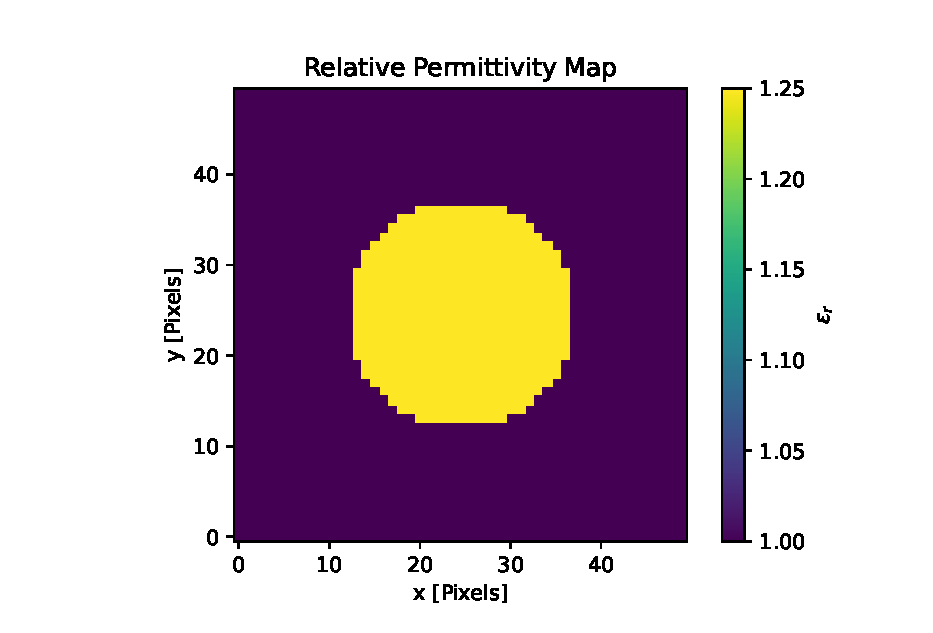
\includegraphics[width=.5\textwidth]{figuras/lcurve_input}}
					\subfloat[]{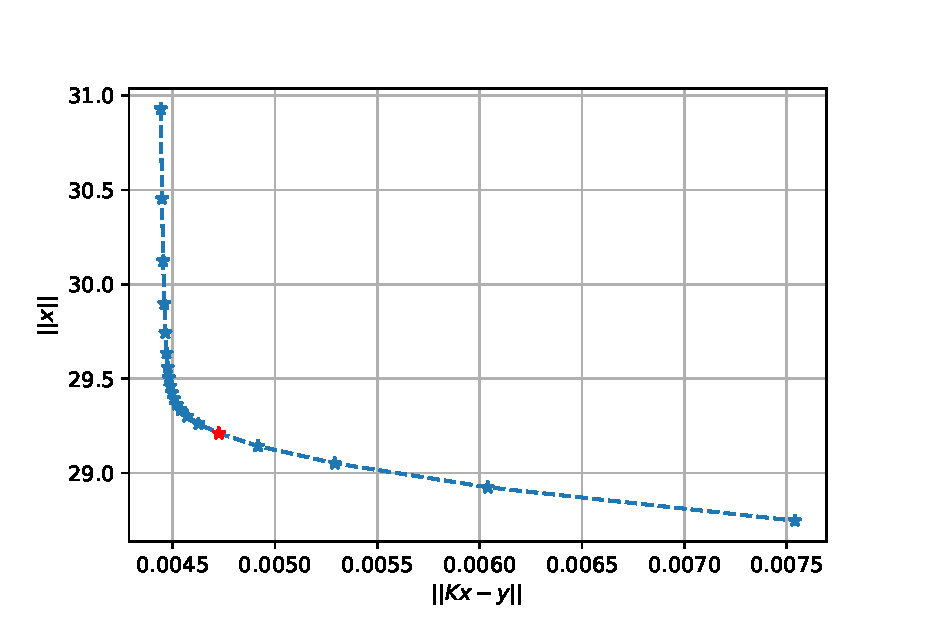
\includegraphics[width=.5\textwidth]{figuras/lcurve}} \\
					\subfloat[]{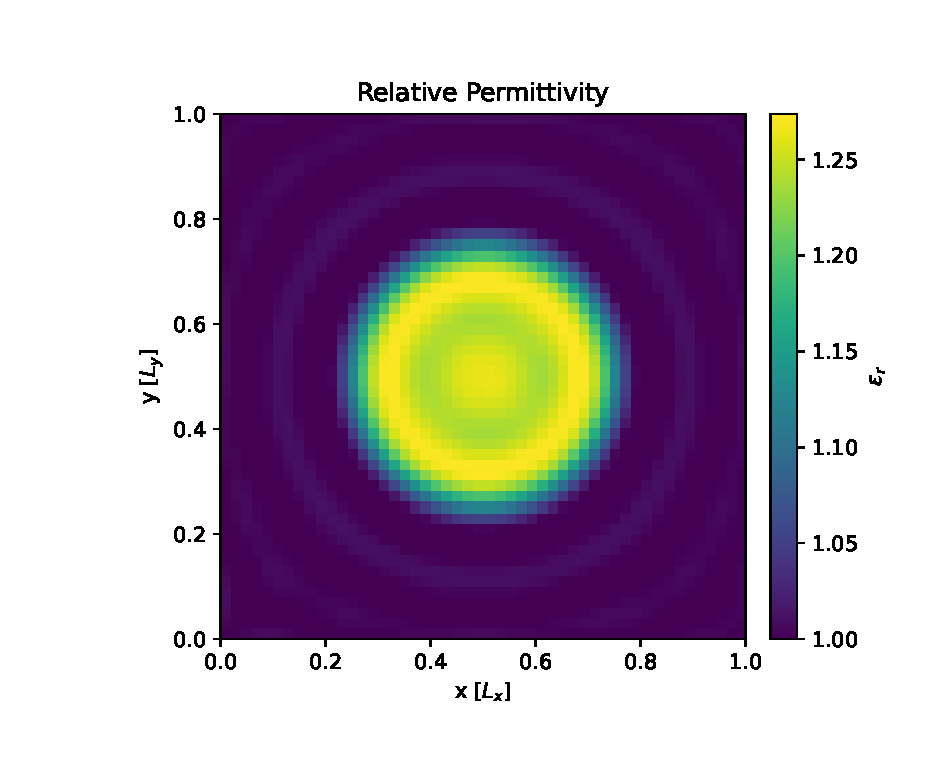
\includegraphics[width=.5\textwidth]{figuras/lcurve_result}}
					\caption[Exemplo de aplicação do Método da Curva-L.]{Example of applying the L-curve Method to a linear problem where it presupposes knowledge of the total field. (a) A simple instance of a contrast dielectric circle $\chi=0.25$ and radius $0.8\lambda_b$. Respecting the degrees of freedom, the scattered field was sampled in 45 positions for 45 incidence angles at a distance of $10\lambda_b$ from the center of the image. (b) L-curve considering 20 values of $\alpha_T$ in a range of $10^{-5}$ a $10^{-2}$. The red dot represents the solution with the shortest normalized distance to the origin. Its $\alpha_T$ value is approximately $2.3357 \times10^{-3}$. (c) Reconstruction of the image using the $\alpha_T$ value from the red dot. No inverse crime was committed since the data were obtained from the analytical solution.}
					\label{fig:3:lcurve}
				\end{figure}
				
			\subsubsection{Trial and Error}\label{chap:methods:linear:tikhonov:trialanderror}
				
				%Por fim, não poderíamos deixar de destacar a abordargem tentativa-e-erro no qual um conjunto de valores de $\alpha_T$ são testados para um problema canônico. A partir destes testes, escolhe-se o valor do resultado mais razoável de acordo com algum critério e utiliza-se esse valor para outros experimentos. Em muitas situações práticas não é necessário o esforço de obter o melhor valor. Basta apenas identificar um intervalo no qual qualquer valor escolhido produza resultados razoáveis. Assim, esta é uma estratégia \textit{a priori}, na qual o valor é definido na entrada do algoritmo.
				Finally, the trial-and-error approach is another popular strategy. A set of $\alpha_T$ values are tested for a canonical problem. The most reasonable result value is chosen according to some criterion, and this value is used for other experiments. In many practical situations, no effort is required to obtain the best value but only identifying a range in which any chosen value produces reasonable results. Therefore, this is \textit{a priori} strategy, in which the value is defined at the input of the algorithm. 
				
		\subsection{The Landweber Regularization}\label{chap:methods:linear:landweber}
				
			%É possível resolver o sistema $\mathcal{K}\{x\}=y$ de forma iterativa se escrevermos a solução $x$ na forma $x=(\mathcal{I}-\alpha_L\mathcal{K}^*\mathcal{K})x+ \alpha_L \mathcal{K}^*\{y\}$ para um $\alpha_L > 0$. Ou seja, a solução é computada iterativamente por:
			It is possible to solve the system $\mathcal{K}\{x\}=y$ iteratively if we write the solution $x$ in the form $x=(\mathcal{I}-\alpha_L\mathcal{K}^*\mathcal{K})x+ \alpha_L \mathcal{K}^*\{y\}$ for an $\alpha_L > 0$. That is, the solution is computed iteratively by:
			\begin{equation}
				x^m=(\mathcal{I}-\alpha_L\mathcal{K}^*\mathcal{K})x^{m-1}+ \alpha_L \mathcal{K}^*\{y\} \label{eq:3:linear:landweber:0}
			\end{equation}
		
			%\noindent cujo o chute inicial pode ser definido como $x^0\coloneqq 0$. Este esquema é semelhante a uma algoritmo de passo descendente no qual o funcional quadrático $||\mathcal{K}\{x\}-y||^2$ é minimizado. O operador de regularização equivalente à definição \eqref{eq:2:inverse:2} pode ser expresso nesse caso como:
			\noindent where the initial guess can be defined as $x^0\coloneqq 0$. This scheme is similar to a descent step algorithm in which the quadratic functional $||\mathcal{K}\{x\}-y||^2$ is minimized. The regularization operator equivalent to the definition \eqref{eq:2:inverse:2} can be expressed in this case as:
			\begin{equation}
				\mathcal{R}_L \coloneqq \alpha_T \sum\limits_{k=0}^{m-1} (\mathcal{I}-\alpha_L\mathcal{K}^*\mathcal{K})^k\mathcal{K}^*,~~ m=1,2,\cdots \label{eq:3:linear:landweber:operator}
			\end{equation}
			
			%No entanto, é necessário definir um critério de parada para o método. Se $\mathcal{K}:X\rightarrow Y$ é um operador linear, compacto e um-pra-um com intervalo denso, então a sequência $x^{m,\delta}$ de \eqref{eq:3:linear:landweber:0}, $m=0,1,2,\cdots$, pode ser rearranjada para:
			However, it is necessary to define a stopping criterion for the method. If $\mathcal{K}:X\rightarrow Y$ is a linear, compact, and one-to-one operator with a dense interval, then the sequence $x^{m,\delta}$ of \eqref{eq:3:linear:landweber:0}, m = $m=0,1,2,\cdots$, can be rearranged to:
			\begin{equation}
				x^{m+1,\delta} = x^{m,\delta} + \alpha_L\mathcal{K}^*\{y-\mathcal{K}\{x^{m,\delta}\}\},~~m=0,1,2,\cdots \label{eq:3:linear:landweber:1}
			\end{equation}
		
			%Dentro dessa definição, pressupõe-se que $||y-y^\delta||\le\delta$, $||y^\delta||\ge r\delta$ para um $r>1$, $\delta\in(0,\delta_0)$ e $0\le \alpha_L \le 1/||\mathcal{K}||^2$. Nestas condições, o critério de parada $||\mathcal{K}\{x^{m,\delta}\}-y^\delta||\le r\delta$ é bem definido, i.e., existe um $m=m(\delta) \in \mathbb{N}_0$ para o qual $||\mathcal{K}\{x^{m,\delta}\}-y^\delta||\le r\delta$. Além disso, é possível demonstrar que essa sequência converge para $x$ e que, se $x=\mathcal{K}^*\{z\}\in\mathcal{K}^*(Y)$ ou $x=\mathcal{K}^*\{\mathcal{K}\{z\}\}\in\mathcal{K}^*\mathcal{K}(X)$ para um $z$ tal que $||z||\le E$, então a ordem de convergência é expressa por \citep{kirsch2011introduction}:
			Within this definition, it is assumed that $||y-y^\delta||\le\delta$, $||y^\delta||\ge r\delta$ for an $r>1$, $\delta\in(0,\delta_0)$ and $0\le \alpha_L \le 1/||\mathcal{K}||^2$. Under these conditions, the stop criterion $||\mathcal{K}\{x^{m,\delta}\}-y^\delta||\le r\delta$ is well defined, i.e., there is a $m=m(\delta) \in \mathbb{N}_0$ for which $||\mathcal{K}\{x^{m,\delta}\}-y^\delta||\le r\delta$. In addition, it is possible to demonstrate that this sequence converges to $x$ and that, if $x=\mathcal{K}^*\{z\}\in\mathcal{K}^*(Y)$ or $x=\mathcal{K}^*\{\mathcal{K}\{z\}\}\in\mathcal{K}^*\mathcal{K}(X)$ for a $z$ such that $||z||\le \Delta$, then the convergence order is expressed by \citep{kirsch2011introduction}:
			\begin{align}
				||x^{m(\delta),\delta}-x|| &\le c\sqrt{\Delta\delta} \label{eq:3:linear:landweber:error1} \\
				||x^{m(\delta),\delta}-x|| &\le c\Delta^{1/3}\delta^{2/3} \label{eq:3:linear:landweber:error2}
			\end{align}
		
			%\noindent respectivamente, para um $c>0$. Em outras palavras, isto significa dizer que a escolha $m(\delta)$ é ótima.
			\noindent respectively, for a $c>0$. In other words, this means that the choice $m(\delta)$ is optimal.
			
			%O método pode ser aplicado no sistema $\mathbf{\bar{E}}^{\mathbf{s},F} = \mathbf{\bar{K}}\boldsymbol{\chi}$ conforme ilustrado no \autoref{alg:landweber}.
			The method can be applied in $\mathbf{\bar{E}}^{\mathbf{s},F} = \mathbf{\bar{K}}\boldsymbol{\chi}$ as illustrated in \autoref{alg:landweber}.
			\begin{algorithm}[!htb]
				\caption{Landweber Method.}
				\label{alg:landweber}
				\KwIn{$\mathbf{\bar{E}}^{\mathbf{s},F}$,$\mathbf{\bar{K}}$, $\alpha_L$, $\delta$}
				\KwOut{$\boldsymbol{\chi}^m$}
				$\boldsymbol{\chi}^0 \leftarrow \mathbf{0}$ \\
				$m\leftarrow 0$ \\
				\While {$||\mathbf{\bar{K}}\boldsymbol{\chi}^m-\mathbf{\bar{E}}^{\mathbf{s},F}|| \le \delta$} {
					$\boldsymbol{\chi}^{m+1} = \boldsymbol{\chi}^m + \alpha_T\mathbf{\bar{K}}^*\left(\mathbf{\bar{E}}^{\mathbf{s},F}-\mathbf{\bar{K}}\boldsymbol{\chi}^m\right)$ \\
					$m \leftarrow m + 1$ \\
				}
			\end{algorithm}
				
		\subsection{The Conjugate Gradient Method}\label{chap:methods:linear:cg}
				
			%O Método do Gradiente Conjugado (CG) é muito popular e aplicado a diversas situações. Nesta seção nos concentraremos na aplicação para problema inversos de equações com operadores limitados, lineares e injetivos entre espaços de Hilbert. Ou seja, dada equação $\mathcal{K}\{x\} = y$ no qual $\mathcal{K} : X \rightarrow Y$ tem as propriedades anteriores comentadas e a adjunta $\mathcal{K}^* : Y \rightarrow X$, definimos o funcional:
			The Conjugated Gradient Method (CG) is very popular and applied to several situations. This section will focus on its formulation for the inverse problem with integral equations considering bounded, linear, and injective operators between Hilbert spaces. Particularly, given equation $\mathcal{K}\{x\} = y$ in which $\mathcal{K} : X \rightarrow Y$ has the previous properties commented and the adjoint $\mathcal{K}^* : Y \rightarrow X$, we define the functional:
			\begin{equation}
				f(x) \coloneqq ||\mathcal{K}\{x\} - y||^2 = \langle \mathcal{K}\{x\} - y, \mathcal{K}\{x\} - y \rangle \label{eq:3:linear:cg:0}
			\end{equation}
		
			%O gradiente de \eqref{eq:3:linear:cg:0} é calculado pela representação de Riesz da derivada de Frechét de $f$, a qual é expressa por:
			The gradient of \eqref{eq:3:linear:cg:0} is calculated by the Riesz representation of the Frechét derivative, which is expressed by:
			\begin{equation}
				\nabla f(x) \coloneqq 2\mathcal{K}^*\{\mathcal{K}\{x\}-y\} \in X \label{eq:3:linear:cg:1}
			\end{equation}
		
			%Auxiliarmente, denominaremos dois elementos $p,q\in X$ como $\mathcal{K}$-conjugados se $\langle \mathcal{K}\{p\}, \mathcal{K}\{q\}=0$. Se $\mathcal{K}$ é um-pra-um, esta definição tem as mesmas propriedades do produto interno em $X$.
			Auxiliary, we will call two elements $p,q\in X$ as $\mathcal{K}$-conjugated if $\langle \mathcal{K}\{p\}, \mathcal{K}\{q\}=0$. If $\mathcal{K}$ is one-to-one, this definition has the same properties as an inner product in $X$.
			
			%A partir destas definições, podemos definir a sequência $x^m$ estabelecida para o CG como:
			From these definitions, we can define the sequence $x^m$ established for CG as:
			\begin{equation}
				x^{m+1} = x^m - t_mp^m \label{eq:3:linear:cg:2}
			\end{equation}
		
			\noindent where:
			\begin{align}
				t_m &= \langle \mathcal{K}\{x^m\}-y, \mathcal{K}\{p^m\} \rangle \label{eq:3:linear:cg:3} \\
				p^{m+1} &\coloneqq \mathcal{K}^*\{\mathcal{K}\{x^{m+1}\}-y\} + \gamma_m p^m \label{eq:3:linear:cg:4} \\
				\gamma_m &\coloneqq \frac{||\mathcal{K}^*\{\mathcal{K}\{x^{m+1}\}-y\}||^2}{||\mathcal{K}^*\{\mathcal{K}\{x^{m}\}-y\}||^2} \label{eq:3:linear:cg:5}
			\end{align}
		
			%Neste método, os gradientes das sequências de $x$ são ortogonais. Além disso, as sequências de direções $p$ são $\mathcal{K}$-conjugadas. Sob certas condições, este algoritmo convergiria para uma solução no qual $\mathcal{K}^*\{\mathcal{K}\{x^{m+1}\}-y\} = 0$. No entanto, quando só é conhecido um $y^\delta\in I$ tal que $||y^\delta-y||\le\delta$, então um critério de parada é o limiar $||\mathcal{K}\{x^{m,\delta}\}-y^\delta||\le\delta$.
			In this method, the gradients of the $x$ sequences are orthogonal. Furthermore, the sequences of directions $p$ are $\mathcal{K}$-conjugated. Under certain conditions, this algorithm converge to a solution in which $\mathcal{K}^*\{\mathcal{K}\{x^{m+1}\}-y\} = 0$. However, when only a $y^\delta\in I$ is known such that $||y^\delta-y||\le\delta$, then a stopping criterion is the threshold $||\mathcal{K}\{x^{m,\delta}\}-y^\delta||\le\delta$.
			
			%A aplicação deste método sobre a equação $\mathbf{\bar{E}}^{\mathbf{s},F}=\mathbf{\bar{K}}\boldsymbol{\chi}$ pode ser vista no \autoref{alg:cg}. Uma das vantagens é que este não depende de um parâmetro de regularização tal qual os métodos de Tikhonov e Landweber. No entanto, o método depende de mais operações.
			The application of this method on $\mathbf{\bar{E}}^{\mathbf{s},F}=\mathbf{\bar{K}}\boldsymbol{\chi}$ can be seen in \autoref{alg:cg}. One of the advantages is that it does not depend on a regularization parameter as Tikhonov and Landweber methods. However, the method depends on more operations.
			\begin{algorithm}[!htb]
				\caption{Conjugated Gradient Method.}
				\label{alg:cg}
				\KwIn{$\mathbf{\bar{E}}^{\mathbf{s},F}$,$\mathbf{\bar{K}}$, $\delta$}
				\KwOut{$\boldsymbol{\chi}^m$}
				$\mathbf{p}^0 \leftarrow -\mathbf{\bar{K}^*}\mathbf{\bar{E}}^{\mathbf{s},F}$ \\
				$\boldsymbol{\chi}^0 \leftarrow \mathbf{0}$ \\
				$m\leftarrow 0$ \\
				\While {$||\mathbf{\bar{K}^*}(\mathbf{\bar{K}}\boldsymbol{\chi}^m-\mathbf{\bar{E}}^{\mathbf{s},F})|| < \delta$} {
					$t_m = \frac{\left[\mathbf{\bar{K}}\boldsymbol{\chi}-\mathbf{\bar{E}}^{\mathbf{s},F}\right]^T\overline{\mathbf{\bar{K}}\mathbf{p}}}{||\mathbf{\bar{K}}\mathbf{p}||^2} $ \\
					$\boldsymbol{\chi}^{m+1} \leftarrow \boldsymbol{\chi}^m - t_m\mathbf{p}^m$ \\
					$\gamma_m = \frac{||\mathbf{\bar{K}^*}\left(\mathbf{\bar{K}}\boldsymbol{\chi}^{m+1}-\mathbf{\bar{E}}^{\mathbf{s},F})\right)||^2}{||\mathbf{\bar{K}^*}\left(\mathbf{\bar{K}}\boldsymbol{\chi}^m-\mathbf{\bar{E}}^{\mathbf{s},F}\right)||^2}$ \\
					$\mathbf{p}^{m+1} = \mathbf{\bar{K}^*}\left(\mathbf{\bar{K}}\boldsymbol{\chi}^{m+1}-\mathbf{\bar{E}}^{\mathbf{s},F}\right) + \gamma_m \mathbf{p}^m$ \\
					$m \leftarrow m + 1$ \\
				}
			\end{algorithm}
				
		\subsection{Spectral Cut-Off}\label{chap:methods:linear:spectral}
					
			%Uma vez que o problema é mal-posto, $\mathbf{\bar{K}}$ é uma matriz cujos os autovalores se aproximam de zero. Quando aplica-se a Decomposição por Valor Singular (SVD) em $\mathbf{\bar{K}}$, o seguinte produto é obtido:
			Since the problem is ill-posed, $\mathbf{\bar{K}}$ is a matrix whose eigenvalues approach zero. When the Single Value Decomposition (SVD) is applied in $\mathbf{\bar{K}}$, the following product is obtained:
			\begin{equation}
				\mathbf{\bar{K}} = \mathbf{\bar{U}}\boldsymbol{\bar{\xi}}\mathbf{\bar{V}}^* \label{eq:3:linear:spectral:0}
			\end{equation}
		
			%\noindent no qual $\mathbf{\bar{U}}$ é uma matriz $N_MN_S\times N_MN_S$ composta por vetores singulares $\mathbf{u}_m$ os quais são ortogonais e unitários; $\mathbf{\bar{V}}$ é uma matriz $N_IN_J\times N_IN_J$ composta por vetores singulares $\mathbf{v}_m$ os quais também são ortogonais e unitários; e $\boldsymbol{\bar{\xi}}$ é a matriz diagonal composta pelos valores singulares $\xi_i$ os quais são reais e em ordem decrescente $\xi_1\ge\xi_2\ge\cdots\ge0$. Matematicamente, a solução $\boldsymbol{\chi}$ pode ser escrita como:
			\noindent in which $\mathbf{\bar{U}}$ is a matrix $N_MN_S\times N_MN_S$ composed of singular vectors $\mathbf{u}_m$ 's which are orthogonal and unitary; $\mathbf{\bar{V}}$ is an $N_IN_J\times N_IN_J$ matrix composed of singular vectors $\mathbf{v}_m$'s which are also orthogonal and unitary; and $\boldsymbol{\bar{\xi}}$ is the diagonal matrix composed of the singular values $\xi_i$'s which are real and place in nonincreasing order  $\xi_1\ge\xi_2\ge\cdots\ge0$. Mathematically, the solution $\boldsymbol{\chi}$ can be written as:
			\begin{equation}
				\boldsymbol{\chi} = \mathbf{\bar{K}}^{-1}\mathbf{\bar{E}}^{\mathbf{s},F} = \sum\limits_{\xi_i\neq0} \frac{1}{\xi_i} \left(\mathbf{u}^*_i\cdot\mathbf{\bar{E}}^{\mathbf{s},F}\right)\mathbf{v}_i \label{eq:3:linear:spectral:1}
			\end{equation}
			
			%Uma vez que $\boldsymbol{\bar{\xi}}$ contém autovalores próximo ou iguais a zero, a operação \eqref{eq:3:linear:spectral:1} é inviável porque pode levar a erros numéricos muito grandes. Isto equivale a dizer que a inversa de $\mathbf{\bar{K}}$ é não-limitada. Por isso, uma alternativa é excluir autovalores menores que um limiar, i.e., $\xi_i<\alpha_{S}$. Assim, \eqref{eq:3:linear:spectral:1} pode ser escrita como um operador de regularização $\mathcal{R}_{SC}$ como:
			Once $\boldsymbol{\bar{\xi}}$ contains eigenvalues close or equal to zero, the operation \eqref{eq:3:linear:spectral:1} is not feasible since it can lead to substantial numerical errors. This is equivalent to saying that the inverse of $\mathbf{\bar{K}}$ is unbounded. Therefore, an alternative is to exclude eigenvalues smaller than a threshold, i.e., $\xi_i<\alpha_{S}$. Then, \eqref{eq:3:linear:spectral:1} can be written as an operator regularization $\mathcal{R}_{SC}$ as:
			\begin{equation}
					\boldsymbol{\chi} = \mathcal{R}_{SC}\{\mathbf{\bar{E}}^{\mathbf{s},F}\} = \sum\limits_{\xi_i>\alpha_{S}} \frac{1}{\xi_i} \left(\mathbf{u}^*_i\cdot\mathbf{\bar{E}}^{\mathbf{s},F}\right)\mathbf{v}_i \label{eq:3:linear:spectral:2}
			\end{equation}
		
			%Este método de regularização é chamado de Corte Espectral e depende da definição de um parâmetro de corte $\alpha_{S}$. Esta solução também conhecida como Norma Mínima. Este método é adequado quando a dimensão das matrizes não são tão grandes, uma vez que o custo computacional para o cálculo dos autovalores e autovetores é elevado. No entanto, o método é muito útil para classificar problemas mal-postos: problemas cujos os autovalores decaem a zero de maneira suave são chamados problemas mildly mal-postos; problemas cujos os autovalores decaem rapidamente a zero são chamados problemas severamente mal-postos.
			This regularization method is called the Spectral Cut-Off and depends on setting a cutting parameter $\alpha_{S}$. This solution is also known as Minimum Norm. This method is suitable when the size of the matrices is not too large since the computational cost for evaluating eigenvectors and eigenvalues may be high. However, the method is convenient for classifying ill-posed problems. The reason is: problems whose eigenvalues drop to zero smoothly are called mildly ill-posed; problems whose eigenvalues rapidly decay to zero are called severely ill-posed problems.
	
	\section{Qualitative Methods}\label{chap:methods:qualitative}
			
		When the contrast estimation is not a required information, qualitative methods are more efficient as they retrieve information about shape and position of scatterers with less computational effort. Even though applications that do not require electric property retrieval seem to be rare, qualitative methods might provide initial solutions for quantitative ones. In the next subsections, some of the qualitative methods are discussed. For a survey of them, readers are referred to \citep{potthast2006survey}.
		
		\subsection{Linear Sampling Method}\label{chap:methods:qualitative:lsm}
			
			The Linear Sampling Method (LSM) is a fast and traditional qualitative method \citep{colton2019inverse,colton1996simple}. If plane waves propagate through the space and the scattered field is sampled in far field conditions, then the scattered field admits the asymptotic behavior given by:
			\begin{equation}
				E_{s_z}(\rho, \theta, \phi) = \frac{e^{-jk_b\rho}}{\sqrt{\rho}}E_{s_\infty}(\theta, \phi) \label{eq:3:qualitative:lsm:kernel}
			\end{equation}
		
			\noindent where $E_{s_\infty}(\theta, \phi)$ is the far-field pattern of the scattered field. For any point $\boldsymbol{\rho}$ in $S$, the following far-field integral holds:
			\begin{equation}
				\int_D d\phi E_{s_\infty}(\theta, \phi) g(\boldsymbol{\rho}, \phi) = \Phi_\infty(\theta, \boldsymbol{\rho}) \label{eq:3:qualitative:lsm:integralequation}
			\end{equation}
		
			\noindent where $\Phi_\infty(\theta, \boldsymbol{\rho})$ is the far-field pattern of the Green's function $-(jk_b^2/4)G^D_{2D}(\theta,\boldsymbol{\rho})$ when the source point is at $\boldsymbol{\rho}$ and the observation point is in the direction $\theta$. $\Phi_\infty(\theta, \boldsymbol{\rho})$ is a function that might be approximated by:
			\begin{equation}
				\Phi_\infty(\theta, \boldsymbol{\rho}) \approx \frac{-j}{4}\sqrt{\frac{2}{\pi k_b}}e^{j\pi/4}e^{jk_b\cos(\theta-\psi)}  \label{eq:3:qualitative:lsm:rhs}
			\end{equation}
		
			\noindent where $\boldsymbol{\rho} = \langle x, y \rangle =  \langle \rho\cos(\psi), \rho\sin(\psi)\rangle$.
			
			The idea behind LSM is to choose an indicator function defined in $S$ which determines if a spatial point belongs or not to a scatterer. The integral equation \eqref{eq:3:qualitative:lsm:integralequation} is solved for $g(\boldsymbol{\rho}, \phi)$ for each $\boldsymbol{\rho}$ in $S$ and each $\phi$ in $D$. The integral equation might be solved through a regularization method (Section \ref{chap:methods:regularization}) after computing the kernel in \eqref{eq:3:qualitative:lsm:integralequation} by \eqref{eq:3:qualitative:lsm:kernel} based on the scattered field data and the right-hand-side \eqref{eq:3:qualitative:lsm:rhs}. The indicator function $I(\boldsymbol{\rho})$ is defined as:
			\begin{equation}
				I(\boldsymbol{\rho}) = ||g(\boldsymbol{\rho})|| = \sqrt{\int_D d\theta |g(\boldsymbol{\rho})|^2} \label{eq:3:qualitative:lsm:indicator}
			\end{equation}
		
			The value indicator function becomes unbound if $\boldsymbol{\rho}$ is not within a scatterer region \citep{colton1996simple}. Therefore, after computing $I(\boldsymbol{\rho})$ for many points in $S$, we are able to recover the scatterer image by verifying if $I(\boldsymbol{\rho})$ tends to infinite or not. Due to discretization of $D$ and $S$ and noise presence in the scattered field data, $I(\boldsymbol{\rho})$ cannot be infinite. Therefore is necessary to set a threshold heuristically for which the background will be set apart from the scatterer.
			
			The LSM is not limited to far-field data. For near-field data, the integral equation \eqref{eq:3:qualitative:lsm:integralequation} is replaced by \citep{cakoni2016qualitative}:
			\begin{equation}
				\int_D d\phi E_{s_z}(\theta, \phi) g(\boldsymbol{\rho}, \phi) = - \frac{jk_b^2}{4} G^D_{2D}(\theta,\boldsymbol{\rho}) \label{eq:3:qualitative:lsm:nearfield}
			\end{equation}
		
			The LSM cannot estimate the dielectric properties of the media. However, it might help the performance of other inversion methods \citep{catapano2007simple,bao2007inverse} and some approximations might be done to turn it into a quantitative method \citep{crocco2012linear}. Further discussion may be found in \citep[see][chap. 5]{chen2017}, \citep{cakoni2016qualitative} and \citep[see][chap. 5]{pastorino2010}.
		
		\subsection{Orthogonality Sampling Method}\label{chap:methods:qualitative:osm}
		
			The Orthogonality Sampling Method (OSM) is another approach to define an indicator function which detects the presence of scatterers \citep{potthast2010study}. Instead of writing it in terms of the solution of the integral equation \eqref{eq:3:qualitative:lsm:integralequation}, the orthogonality between far-field data and an exponential function is tested. Another interpretation is the superposition of plane waves back into the region of the scatterer, which is a very known idea. Mathematically, the orthogonality is tested according to \citep{potthast2010study,akinci2016nearfield}:
			\begin{equation}
				E_{s_z}^{red} (\boldsymbol{\rho}, \theta) = \int_D d\phi E_{s_\infty}(\theta,\phi)e^{-jk_b\rho\cos(\theta-\psi)} = \int_D d\phi \frac{e^{-jk_b/4}}{\sqrt{8\pi k_b}} E_{s_z}(\theta, \phi) e^{-jk_b\rho\cos(\theta-\psi)} \label{eq:3:qualitative:osm:farfield:equation}
			\end{equation}
		
			\noindent where $E_{s_z}^{red}$ is know as the reduced scattered field. The indicator function is defined as:
			\begin{equation}
				I(\boldsymbol{\rho}) = \int_D d\theta |E_{s_z}^{red} (\boldsymbol{\rho}, \theta)|^2 \label{eq:3:qualitative:osm:farfield:indicator}
			\end{equation}
		
			Therefore, the indicator function computation does not require solving an integral equation. Rather it depends on integrating reduced scattered field. The maxima of the function is used to identify the scatterers. Near-field data is also compatible with the method. However, the reduced scattered field definition needs to be adapted \citep{akinci2016nearfield}:
			\begin{equation}
				E_{s_z}^{red} (\boldsymbol{\rho}, \theta) = = \int_D d\phi E_{s_z}(\theta, \phi) K^{TM}(\theta, \boldsymbol{\rho}) \label{eq:3:qualitative:osm:nearfield:equation}
			\end{equation}
		
			\noindent where:
			\begin{equation}
				K^{TM}(\theta, \boldsymbol{\rho}) = \frac{-2j}{\pi R_O}\sum\limits_{n=-\infty}^{\infty} \frac{J_n(k_b\rho)}{H_n^{(2)}(k_bR_O)}e^{-jn(\theta-\psi)} \label{eq:3:qualitative:osm:nearfield:indicator}
			\end{equation}
		
			\cite{akinci2016nearfield} stated that the reduced scattered field is directly related to the electrical properties of the scatterers. \cite{bevacqua2020physical} went further and concluded that the reduced scattered field can be related to the radiating component of the induced currents. As a consequence, OSM is able to image discontinuities within unknown scatterers and identify regions with different electromagnetic properties, differently than other qualitative methods.
			
	\section{Deterministic Quantitative Methods}\label{chap:methods:deterministic}
			
		%Considerando agora o problema não-linear, existe uma classe de métodos que resolvem as equações de forma determinística, i.e., sem o recurso de operações aleatórias. Esta classe é a mais popular na literatura do problema, a qual possui uma grande quantidade de métodos. Nesta seção serão discutidos tanto métodos tradicionais que foram relevantes na história da literatura quanto aqueles que são considerados estado-da-arte.
		Now considering the nonlinear and quantitative problem, there is a class of methods that solve the equations in a deterministic fashion, i.e., without the use of random operations. This class is the most popular in the problem literature, which has a large number of methods. This section will discuss both traditional methods relevant to the history of literature and those that are considered state-of-the-art.
				
		\subsection{The Born Iterative Method}\label{chap:methods:deterministic:bim}
					
			%Um dos primeiros métodos a se popularizar foi proposto por \cite{wang1989iterative}. Pressupondo que o meio de fundo é conhecido e homogêneo, os autores proporam uma abordagem iterativa onde cada iteração era equivalente à solução por séries de Neumann. A partir de uma estimativa inicial da função contraste, o processo iterativo se baseia em obter uma solução para o campo total através de um resolvedor direto e resolver o problema linear inverso a partir desta estimativa do campo para atualizar a estimativa da função contraste (\autoref{alg:bim}). Portanto, o método se baseia em uma estratégia de linearização do problema, i.e., dividindo o problema em subproblemas lineares.
			One of the first methods to become popular was proposed by \cite{wang1989iterative}. Assuming a homogeneous background medium, the authors proposed an iterative approach where each iteration was equivalent to the solution by Neumann series. From an initial estimate of the contrast function, the iterative process is based on obtaining a solution for the total field through a direct solver and solving the inverse linear problem to update the estimate of the contrast function based on the current estimate of the total field (\autoref{alg:bim}). Therefore, the method is based on a linearization strategy, i.e., dividing the problem into two linear subproblems.
			
			\begin{algorithm}[!htb]
				\caption{Born Iterative Method.}
				\label{alg:bim}
				\KwIn{$\mathbf{\bar{E}^s}$, $\mathbf{\bar{E}^i}$, $\mathbf{\bar{G}^D}$, $\mathbf{\bar{G}^S}$}
				\KwOut{$\boldsymbol{\bar{\chi}}$, $\mathbf{\bar{E}}$}
				Compute an initial guess $\boldsymbol{\bar{\chi}^0}$ based on available information \\
				$m\leftarrow0$ \\
				\While{some criterion is not reached} {
					Update $\mathbf{\bar{E}}^m$ based on the current $\boldsymbol{\bar{\chi}}^m$ estimation \\
					Update $\boldsymbol{\bar{\chi}}^m$ based on the current $\mathbf{\bar{E}}^m$ estimation \\
				}
			\end{algorithm}
		
			%Originalmente, os autores utilizaram o Método dos Momentos definido por \cite{richmond1965scattering} como resolvedor direto e a Regularização de Tikhonov com parâmetro escolhido por tentativa-e-erro como resolvedor inverso. No entanto, outros resolvedores podem ser utilizados de forma que o método se tornou uma estrutura genérica onde muitas estratégias podem ser definidas, como por exemplo, os outros regularizadores definidos na seção anterior, o uso de funções de Conjunto de Nível \citep{shah2018fast} e Programação Quadrática \citep{batista2021quadratic}. Esta última técnica pode ser adequada para acoplar diferentes formas de regularização através da formulação da função objetivo.
			Initially, the authors used the Method of Moments defined by Richmond (1965) as the forward solver and Tikhonov's Regularization with a parameter chosen by trial-and-error as an inverse solver. However, other solvers can be used in such a way that the method has become a generic structure where many strategies can be defined, for example, the other regularizers defined in the previous section, the use of Level Set functions \citep{shah2018fast} and Quadratic Programming \citep{batista2021quadratic}. This latter technique may be suitable for coupling different forms of regularization through the objective function definition.
			
			%No artigo original, os autores chamaram o algoritmo de Método de Newton Modificado, uma vez que o processo iterativo pode ser comparado com a definição de uma direção busca para uma solução corrente. No entanto, o algoritmo ficou conhecido na literatura como Método Iterativo de Born (BIM) uma vez que o objetivo era propor uma solução para os casos onde a Aproximação de Born não era válida. Embora a intenção fosse essa, o algoritmo também tem limites em relação à aplicação em casos de alto contraste. Geralmente, a solução inicial é determinada pela Aproximação de Born, e por isso, a convergência do algoritmo pode ficar comprometida em situações de espalhadores fortes. \cite{moghaddam1993study} se aprofundou nesta questão mostrando boas reconstruções para objetos com diâmetro de $8.5\lambda_b$ em relação à frequência central de operação\footnote{Neste trabalho, os autores formularam o problema no domínio do tempo. Este tipo de formulação tem a vantagem de considerar mais frequências no processo de inversão.} e contraste $\chi=1$. No entanto, não existe na literatura uma medição robusta sobre a relação entre contraste e tamanho que o BIM é capaz de suportar. Destaca-se também a comparação entre o BIM e Método de Tarantola realizada por \cite{moghaddam1991comparison} no qual concluiu-se que, embora o Método de Tarantola tenha um custo computacional menor do que o BIM, este último pode convergir mais rápido e ser mais robusto com objetos que têm pontas.
			In the original article, the authors called the Modified Newton Method algorithm since the iterative process can be compared with the definition of a search direction for a current solution. However, the algorithm was known in the literature as the Born Iterative Method (BIM) since the objective was to propose a solution for cases where the Born Approximation was not valid. Although this was the intention, the algorithm also has limits concerning the application in cases of high contrast. Generally, the initial solution is determined by the Born Approximation, and therefore, the convergence of the algorithm can be compromised when strong scatterers are considered. \cite{moghaddam1993study} went deeper into this issue showing good reconstructions for objects with a diameter of $8.5\lambda_b$ in relation to the central frequency of operation\footnote{In this work, the authors formulated the problem in the time domain. This type of formulation has the advantage of considering more frequencies in the inversion process.} and contrast $\chi=1$. However, there is no robust measurement in the literature on the relationship between contrast and size that BIM can support. Also noteworthy is the comparison between BIM and the Tarantola Method carried out by \cite{moghaddam1991comparison}. Although Tarantola's Method has a lower computational cost than BIM, the latter can converge faster and be more robust with objects that have edges.
			
			%É necessário destacar também que implementações do BIM as quais utilizam regularizadores baseados em parâmetros precisam de estratégias para a escolha do seu valor. Assim como no artigo original, muitos outros trabalhos na literatura os quais utilizam este tipo de regularizador na linearização do problema inverso, escolhem um valor fixo para todas as iterações baseados em tentativa-e-erro \citep{chew1995frequency,yao1997frequency,li2004three,chew1994inversion,batista2021quadratic}. De fato, a escolha não é trivial e não há uma regra simples para a escolha ótima no problema não-linear \citep{engl1988convergence}.
			It is also necessary to highlight that BIM implementations that use parameter-based regularizers need strategies to choose their value. As in the original article, many other works in the literature that use this kind of regularizer choose a fixed value for all iterations based on trial-and-error strategy \citep{chew1995frequency,yao1997frequency,li2004three,chew1994inversion,batista2021quadratic}. In fact, the choice is not trivial, and there is no simple rule for the optimal choice in the nonlinear problem \citep{engl1988convergence}.
			
			%No entanto, existem estratégias para uma definição dinâmica de $\alpha_T$ ao longo processo iterativo do BIM. No trabalho original, os autores afirmam que valores altos $\alpha_T$ são importantes para evitar componentes de alta frequência na função contraste a qual estão associadas com ruídos na imagem. No entanto, essa componentes também podem ser importantes para a reconstruções vértices do objeto. Conforme defendido por \cite{moghaddam1992nonlinear}, os pequenos autovalores em $\mathbf{\bar{K}}$ podem contribuir para uma melhor reconstrução dos contornos quando a função contraste já estiver suficientemente suave durante o processo de reconstrução. Por isso eles propõem que, nas primeiras iterações do BIM, sejam utilizados valores altos de $\alpha_T$ para filtrar variações bruscas na função contraste; a partir daí, $\alpha_T$ seria diminuído para melhorar os contornos da imagem. Conforme explicam, esta estratégia é equivalente a começar procurando soluções num subespaço menor e ir expandindo ao longo das iterações. Também foram propostas na literatura regras para esta adaptação de $\alpha_T$ \citep{lavarello2008study,joachimowicz1991inverse,franchois1997microwave,zaiping2000variational}. Semelhantemente, metodologias que consideram os dados do campo espalhado em múltiplas frequências sugerem um uso dinâmico similar, i.e., começar com as frequências mais baixas e terminar com as mais altas \citep{chew1995frequency,batista2021quadratic}.
			However, there are strategies for a dynamic definition of $\alpha_T$ throughout the iterative process. In the original work, the authors state that high $\alpha_T$ values are essential to avoid high-spatial-frequency components in the contrast function associated with noise in the image. However, these components can also be necessary for the object's vertex reconstructions. As advocated by \cite{moghaddam1992nonlinear}, the small eigenvalues in $\mathbf{\bar{K}}$ can better reconstruct the contours when the contrast function is already sufficiently smooth during the reconstruction process. For this reason, they propose that, in the first BIM iterations, high values of $\alpha_T$ should be used to filter out sudden variations in the contrast function; after that, $\alpha_T$ would be decreased to improve the contours of the image. As they explain, this strategy is equivalent to start looking for solutions in a smaller subspace and expanding over iterations. Rules for this adaptation of $\alpha_T$ have also been proposed in the literature \citep{lavarello2008study,joachimowicz1991inverse,franchois1997microwave,zaiping2000variational}. Similarly, methodologies that consider scattered field data with multiple frequencies suggest a similar dynamic use, i.e., starting with the lowest frequencies and ending with the highest ones \citep{chew1995frequency,batista2021quadratic}.
							
		\subsection{The Distorted Born Iterative Method}\label{chap:methods:deterministic:dbim}
				
			%Os mesmos autores do BIM também publicaram no ano seguinte uma metodologia alternativa \citep{chew1990reconstruction}. Nessa nova abordagem, as equações do subproblema inverso não são resolvidas para $\chi$, e sim, para uma variação $\Delta\chi$. Desta forma, a função contraste é atualizada a cada iteração $t$ pela forma $\chi^t = \chi^{t-1} + \Delta\chi$. No entanto, para resolver o subproblema inverso em função de $\Delta\chi$ é necessário resolver a equação integral considerando um meio de fundo não-homogêneo conforme \eqref{eq:app:green:28}. Por isso, a cada iteração, a função de Green para o meio não-homogêneo \eqref{eq:app:green:29} precisa ser calculada levando a estimativa do contraste do final da iteração anterior como meio de fundo.
			The same BIM authors also published an alternative methodology the following year \citep{chew1990reconstruction}. In this new approach, the inverse subproblem equations are not solved for $\chi$ but a variation $\Delta\chi$. Consequently, the contrast function is updated at each iteration $t$ by the form $\chi^t = \chi^{t-1} + \Delta\chi$. However, to solve the inverse subproblem as a function of $\Delta\chi$, it is necessary to solve the integral equation considering a inhomogeneous background medium according to \eqref{eq:app:green:28}. Therefore, at each iteration, Green's function for the inhomogeneous medium \eqref{eq:app:green:29} needs to be calculated, taking the contrast estimate at the end of the previous iteration as the background medium.
					
			%Para calcularmos a função de Green não-homogênea em um problema bidimensional para um par de pontos $\brho_{m}$ e $\brho_{n}$, é necessário considerarmos a seguinte equação:
			The following equation must be considered for calculating the inhomogeneous Green function in a two-dimensional problem for a pair of points $\brho_{m}$ e $\brho_{n}$:
			\begin{equation}
				G_{in}(\brho_{m},\brho_{n}) = G_{2D}(\brho_{m},\brho_{n}) - \frac{jk_0^2}{4} \int_{S}dS^{\prime}~ G_{2D}(\brho_m,\brhop)\chi(\brhop)G_{in}(\brhop,\brho_n) \label{eq:3:deterministic:dbim:0}
			\end{equation}
				
			%\noindent onde $G_{2D}(\brho_{m},\brho_{n})=H^{(2)}_0(k_0|\brho_m-\brho_n|)$. Pelo teorema da reciprocidade, podemos reescrever \eqref{eq:3:deterministic:dbim:0} como:
			\noindent where $G_{2D}(\brho_{m},\brho_{n})=H^{(2)}_0(k_0|\brho_m-\brho_n|)$. By the reciprocity theorem, we can rewrite \eqref{eq:3:deterministic:dbim:0} as:
			\begin{equation}
				G_{in}(\brho_{n},\brho_{m}) = G_{2D}(\brho_{n},\brho_{m}) - \frac{jk_0^2}{4} \int_{S}dS^{\prime}~ G_{2D}(\brho_n,\brhop)\chi(\brhop)G_{in}(\brhop,\brho_m) \label{eq:3:deterministic:dbim:1}
			\end{equation}
		
			%Seguindo a mesma discretização de \eqref{eq:3:discretization:collocation:3}-\eqref{eq:3:discretization:collocation:7}, a região $S$ será dividida em $N_IN_J$ elementos e o valor de $G_{in}$ será amostrado nestes pontos:
			Following the same discretization of \eqref{eq:3:discretization:collocation:3}-\eqref{eq:3:discretization:collocation:7}, the $S$ region will be divided into $N_IN_J$ elements, and the value of $G_{in}$ will be sampled at these points:
			\begin{equation}
				G_{in}(\brho_{n},\brho_{m}) = G_{2D}(\brho_{n},\brho_{m}) - \sum\limits_{p=1}^{N_I}\sum\limits_{q=1}^{N_J} \chi(\brho_{pq}) G_{in}(\brho_{pq},\brho_{m}) \left(\frac{jk_0^2}{4}\int_{S_k}dS^{\prime}~ G_{2D}(\brho_n,\brhop)\right) \label{eq:3:deterministic:dbim:2}
			\end{equation}
		
			%Note que a integral entre parênteses é equivalente a \eqref{eq:3:discretization:collocation:1}. Por isso, ela pode ser substituída como foi feito em \eqref{eq:3:discretization:collocation:9}. Por isso, \eqref{eq:3:deterministic:dbim:2} pode ser escrita como um sistema de equações lineares:
			Note that the integral in parentheses is equivalent to  \eqref{eq:3:discretization:collocation:1}. So it can be replaced as was done in \eqref{eq:3:discretization:collocation:9}. Therefore, \eqref{eq:3:deterministic:dbim:2} can be written as a system of linear equations:
			\begin{equation}
				G^{in}_{nm} = G^{2D}_{nm} - \sum\limits_{p=1}^{N_I}\sum\limits_{q=1}^{N_J} \chi_{pq}G^{in}_{pqm} G^{2D}_{npq} \label{eq:3:deterministic:dbim:3}
			\end{equation}
		
			%\noindent no qual $G^{in}_{nm} = G_{in}(\brho_{n},\brho_{m})$, $G^{2D}_{nm}=G_{2D}(\brho_{n},\brho_{m}) $, $\chi_{pq}=\chi(\brho_{pq})$, $G^{in}_{pqm}=G_{in}(\brho_{pq},\brho_{m})$ e $G^{2D}_{npq}$ é o equivalente a \eqref{eq:3:discretization:collocation:1}.
			\noindent in which $G^{in}_{nm} = G_{in}(\brho_{n},\brho_{m})$, $G^{2D}_{nm}=G_{2D}(\brho_{n},\brho_{m}) $, $\chi_{pq}=\chi(\brho_{pq})$, $G^{in}_{pqm}=G_{in}(\brho_{pq},\brho_{m})$ and $G^{2D}_{npq}$ is equivalent to \eqref{eq:3:discretization:collocation:1}.
			
			%O objetivo é determinar a função de Green não-homogênea $G^{in}$ para que essa substitua $G^D_{2D}$ em \eqref{eq:3:definition:4}. Portanto, $\brho_m$ é um ponto de medição do campo em $D$. Já $\brho_n$ é um ponto da discretização em $S$. Por isso, \eqref{eq:3:deterministic:dbim:3} deve ser reescrita como:
			The objective is to determine the inhomogeneous Green function $G^{in}$ so that this replaces $G^D_{2D}$ in \eqref{eq:3:definition:4}. Therefore, $\brho_m$ is a measurement point of the field in $D$. Now $\brho_n$ is a point of discretization in $S$. Therefore, \eqref{eq:3:deterministic:dbim:3} should be rewritten as:
			\begin{equation}
				G^{in}_{mij} = G^{2D}_{mij} - \sum\limits_{p=1}^{N_I}\sum\limits_{q=1}^{N_J} \chi_{pq}G^{in}_{mpq} G^{S}_{ijpq} \label{eq:3:deterministic:dbim:4}
			\end{equation}
		
			%\noindent no qual $G^{in}_{mij} = G_{in}(\theta_m,x_i,y_j)$, $G^{2D}_{mij}$ é o mesmo que \eqref{eq:3:definition:9} para $\theta_m$, $x_i$, $y_j$; $\chi_{pq}=\chi(x_p, y_q)$ e $G^{S}_{npq}$ é o mesmo de \eqref{eq:3:discretization:collocation:9}. Desta forma, \eqref{eq:3:deterministic:dbim:4} pode ser escrita em forma matricial:
			\noindent where $G^{in}_{mij} = G_{in}(\theta_m,x_i,y_j)$, $G^{2D}_{mij}$ is the same of \eqref{eq:3:definition:9} for $\theta_m$, $x_i$, $y_j$; $\chi_{pq}=\chi(x_p, y_q)$ and $G^{S}_{npq}$ is equivalent to \eqref{eq:3:discretization:collocation:9}. Consequently, \eqref{eq:3:deterministic:dbim:4} might be rewrite in a matrix fashion:
			\begin{equation}
				\left(\mathbf{\bar{I}} - \mathbf{\bar{G}^S}\boldsymbol{\bar{\chi}}\right)\mathbf{\bar{G}^{in}} = \mathbf{\bar{G}^{2D}} \label{eq:3:deterministic:dbim:5}
			\end{equation}
		
			%\noindent no qual as matrizes $\mathbf{\bar{G}^{in}}$ e $\mathbf{\bar{G}^{2D}} $ são definidas de maneira similar a $\mathbf{\bar{G}^D}$. \eqref{eq:3:deterministic:dbim:5} pode ser resolvida a partir de técnicas para solução de sistemas lineares se transformarmos $\mathbf{\bar{G}^{in}}$ e $\mathbf{\bar{G}^{2D}}$ em vetores-coluna.
			\noindent in which the matrices $\mathbf{\bar{G}^{in}}$ and $\mathbf{\bar{G}^{2D}} $ are defined similarly to $\mathbf{\bar{G}^D}$. \eqref{eq:3:deterministic:dbim:5} can be solved using techniques for solving linear systems if we transform $\mathbf{\bar{G}^{in}}$ e $\mathbf{\bar{G}^{2D}}$ in column-vectors.
			
			%Portanto, o método proposto por \cite{chew1990reconstruction} precisa resolver \eqref{eq:3:deterministic:dbim:5} a cada iteração substituindo a matriz $\boldsymbol{\bar{\chi}}$ pela solução da função contraste obtida no final da iteração anterior. Convém destacar que muitos resolvedores diretos já utilizam a matriz $(\mathbf{\bar{I}} - \mathbf{\bar{G}^S}\boldsymbol{\bar{\chi}})$ em suas formulações, tal como o Método dos Momentos \citep{richmond1965scattering}. Além disso, é preciso levar em consideração os dados do campo espalhado em cada iteração. Uma vez que a equação integral deve ser resolvida para $\Delta\chi$, o campo espalhado na esquerda de \eqref{eq:3:discretization:collocation:10} de ser subtraído pela estimativa atual feita no resolvedor direto. Ou seja, o resolvedor direto calcula o campo total $\mathbf{\bar{E}}^t$ e o espalhado correspondente $\mathbf{\bar{E}}^{\mathbf{s},t}$. Desta forma, o resolvedor inverso determina $\Delta\chi$ a partir de $\mathbf{\bar{E}}^t$, $\mathbf{\bar{G}}^{\mathbf{in},t}$ e $\Delta\mathbf{\bar{E}^s} = \mathbf{\bar{E}^s} - \mathbf{\bar{E}}^{\mathbf{s},t}$.
			Therefore, the method proposed by \cite{chew1990reconstruction} needs to solve \eqref{eq:3:deterministic:dbim:5} at each iteration, replacing the $\boldsymbol{\bar{\chi}}$ matrix with the solution of the contrast function obtained at the end of the previous iteration. It should be noted that many forward solvers already use the matrix $(\mathbf{\bar{I}} - \mathbf{\bar{G}^S}\boldsymbol{\bar{\chi}})$ in their formulations, such as the Method of Moments \citep{richmond1965scattering}. In addition, it is necessary to take into account the scattered field data in each iteration. Since the integral equation must be solved for $\Delta\chi$, the scattered field at the left-hand side of \eqref{eq:3:discretization:collocation:10} must be subtracted from the current estimate done by the forward solver. That is, the forward solver calculates the total field $\mathbf{\bar{E}}^t$ and the corresponding scattered field $\mathbf{\bar{E}}^{\mathbf{s},t}$. Thus, the inverse solver determines $\Delta\chi$ from $\mathbf{\bar{E}}^t$, $\mathbf{\bar{G}}^{\mathbf{in},t}$, and $\Delta\mathbf{\bar{E}^s} = \mathbf{\bar{E}^s} - \mathbf{\bar{E}}^{\mathbf{s},t}$.
			
			%Esta metodologia é conhecida como Método Iterativo de Born Distorcido (DBIM) uma vez que é baseada na Distorted-Wave Born Approximation (DWBA), a qual é semelhante à Aproximação de Born. No entanto, a diferença é que ao invés de aproximar o campo total pelo campo incidente num meio homogêneo, DWBA considera o campo total do fundo não-homogêneo. O funcionamento básico do DBIM pode ser visualizado no \autoref{alg:dbim}.
			This methodology is known as the Distorted Born Iterative Method (DBIM) since it is based on the Distorted-Wave Born Approximation (DWBA), similar to BA. However, the difference is that instead of approximating the total field by the incident one in a homogeneous medium, DWBA considers the total field due to an inhomogeneous medium. The basic operation of DBIM can be shown in \autoref{alg:dbim}.
			\begin{algorithm}[!htb]
				\caption{Distorted Born Iterative Method.}
				\label{alg:dbim}
				\KwIn{$\mathbf{\bar{E}^s}$, $\mathbf{\bar{G}^{2D}}$, $\mathbf{\bar{G}^S}$}
				\KwOut{$\boldsymbol{\bar{\chi}}$, $\mathbf{\bar{E}}$}
				Compute an initial guess $\boldsymbol{\bar{\chi}^0}$ based on available information \\
				$t\leftarrow0$ \\
				\While{some criterion is not reached} {
					Solve $\left(\mathbf{\bar{I}} - \mathbf{\bar{G}^S}\boldsymbol{\bar{\chi}}^t\right)\mathbf{\bar{G}}^{\mathbf{in},t} = \mathbf{\bar{G}^{2D}}$ for $\mathbf{\bar{G}}^{\mathbf{in},t}$ \\
					Solve the direct problem for $\mathbf{\bar{E}}^t$ and $\mathbf{\bar{E}}^{\mathbf{s},t}$ \\
					$\Delta\mathbf{\bar{E}^s} = \mathbf{\bar{E}}^s - \mathbf{\bar{E}}^{\mathbf{s},t}$ \\
					Solve the inverse linear problem $\Delta\mathbf{\bar{E}^s} = \mathbf{\bar{G}}^{\mathbf{in},t}\Delta\boldsymbol{\bar{\chi}}\mathbf{\bar{E}}^t$ for $\Delta\boldsymbol{\bar{\chi}}$\\
					$\boldsymbol{\bar{\chi}}^t \leftarrow \boldsymbol{\bar{\chi}}^{t-1} + \Delta\boldsymbol{\bar{\chi}}^t$ \\
					$t\leftarrow t+1$\\
				}
			\end{algorithm}
		
			%Uma vez que o método resolve o subproblema inverso levando em consideração o erro na aproximação do campo espalhado, o algoritmo pode divergir a partir do momento em que o erro $\Delta\mathbf{\bar{E}^s}$ começa a ficar próximo da quantidade de ruído nos dados. Por causa disso, um critério de parada razoável para o método é quando o resíduo da equação começar a crescer de uma iteração para outra. Por esse mesmo motivo, os autores demonstraram que o DBIM é menos robusto que o BIM quando os dados estão contaminados por ruído. No entanto, os experimentos demonstraram uma diferença significativa na velocidade de convergência do método.
			Once the method solves the inverse subproblem taking into account the error in approaching the scattered field, the algorithm may diverge from when the error $\Delta\mathbf{\bar{E}^s}$ starts to be close to the noise level in the data. Therefore, a reasonable stopping criterion is ending the algorithm when the residual starts to grow from one iteration to another. Due to this condition, the authors demonstrated that DBIM is less robust than BIM in noisy data situations. However, the experiments showed a significant difference in the convergence speed, i.e., DBIM converges earlier than BIM.
			
			%Por fim, vale à pena destacar que o DBIM é uma metodologia equivalente ao Método de Newton-Kantorovich (NK) \citep{remis2000equivalence}. NK é uma extensão do método de Newton para resolver equações não-lineares em espaços funcionais. Sua principal diferença é que, além de determinar $\Delta\boldsymbol{\chi}$ tal que esse satisfaça $\Delta\mathbf{\bar{E}^s} = \mathbf{\bar{G}}^{\mathbf{in},t}\Delta\boldsymbol{\bar{\chi}}\mathbf{\bar{E}}^t$, o método também requer que $\Delta\boldsymbol{\chi}$ satisfaça simultaneamente $\Delta\mathbf{\bar{E}^s} = \mathbf{\bar{G}^S}(\mathbf{\bar{I}} - \mathbf{\bar{G}^S}\boldsymbol{\bar{\chi}}^t)^{-1} \Delta\boldsymbol{\bar{\chi}}\mathbf{\bar{E}}^t$. No entanto, isto é equivalente ao cálculo da função de Green em \eqref{eq:3:deterministic:dbim:5}. Conforme afirmado por \cite{chen2017}, estas metodologias são equivalentes a determinar um gradiente para a função contraste baseada na derivada de Frechét do resíduo de $\mathbf{\bar{E}^s}+\mathbf{\bar{G}^D}\boldsymbol{\bar{\chi}}(\mathbf{\bar{I}}+\mathbf{\bar{G}^S}\boldsymbol{\bar{\chi}})^{-1}\mathbf{\bar{E}^i}$. Este resíduo pode ser obtido através da substituição de $\mathbf{\bar{E}}$ em \eqref{eq:3:discretization:collocation:10} pela solução de \eqref{eq:3:discretization:collocation:11} como problema direto. Uma vez que o problema é não-linear e possui muitos mínimos locais \citep{chen2017}, tanto DBIM como NK não garantem a convergência para ótimo global representado pelo mínimo resíduo das equações.
			Finally, it is worth noting that DBIM is a methodology equivalent to Newton-Kantorovich (NK) method \citep{remis2000equivalence}. NK is an extension of Newton's method for solving nonlinear equations in functional spaces. Its main difference is that, in addition to determining $\Delta\boldsymbol{\chi}$ such that it satisfies $\Delta\mathbf{\bar{E}^s} = \mathbf{\bar{G}}^{\mathbf{in},t}\Delta\boldsymbol{\bar{\chi}}\mathbf{\bar{E}}^t$, the method also requires that $\Delta\boldsymbol{\chi}$ simultaneously satisfy $\Delta\mathbf{\bar{E}^s} = \mathbf{\bar{G}^S}(\mathbf{\bar{I}} - \mathbf{\bar{G}^S}\boldsymbol{\bar{\chi}}^t)^{-1} \Delta\boldsymbol{\bar{\chi}}\mathbf{\bar{E}}^t$. However, this is equivalent to calculating Green's function in \eqref{eq:3:deterministic:dbim:5}. As stated by \cite{chen2017}, these methodologies are equivalent to determining a gradient for the contrast function based on the Frechét derivative of the $\mathbf{\bar{E}^s}+\mathbf{\bar{G}^D}\boldsymbol{\bar{\chi}}(\mathbf{\bar{I}}+\mathbf{\bar{G}^S}\boldsymbol{\bar{\chi}})^{-1}\mathbf{\bar{E}^i}$. This residue can be obtained by replacing $\mathbf{\bar{E}}$ in \eqref{eq:3:discretization:collocation:10} with the solution of \eqref{eq:3:discretization:collocation:11} as a forward problem. Since the problem is nonlinear and has many local minima \citep{chen2017}, both DBIM and NK do not guarantee the convergence to a global optimum represented by the minimum residue of equations.

		\subsection{The Variational Born Iterative Method}\label{chap:methods:deterministic:vbim}
			
			%\cite{zaiping1998hybrid} realizaram experimentos considerando o acoplamento dentro BIM com o DBIM. Especificamente, o DBIM foi utilizado nas primeiras iterações enquanto o BIM foi utilizado nas últimas. O objetivo era unir as melhores características de cada método, i.e., a rápida convergência do DBIM e a estabilidade do BIM. No entato, os autores verificaram que esta versão híbrida, chamada Hybrid Born Iterative Method (HBIM), muitas operações para o acoplamento destas duas metodologias.
			\cite{zaiping1998hybrid} carried out experiments considering the coupling between BIM and DBIM. Specifically, DBIM was used in the first iterations, while BIM, in the latter. The goal was to bring together the best features of each method, i.e., the rapid convergence of DBIM and BIM stability. However, the authors found that this hybrid version, called Hybrid Born Iterative Method (HBIM), took too many operations for coupling these two methodologies.
			
			%Posteriormente, \cite{zaiping2000variational} proporam substituir o DBIM por um método chamado Variational Born Iterative Method (VBIM) no qual, sua diferença para o DBIM, era que a função de Green não era atualizada em cada iteração. Ou seja, a função de Green para o meio homogêneo era utilizada em todo processo. Isto reduz drasticamente a quantidade de operações do método. Os experimentos com objetos condutivos indicaram uma diferença de 20\% na eficiência computacional\footnote{Neste trabalho, os autores não explicaram bem a definição do conceito de eficiência computacional. Não há nenhum gráfico ou tabela que explique melhor o significado deste dado. Além disso, BIM, DBIM e VBIM foram comparados em apenas três instâncias, o que é muito pouco para inferir excluir o viés da escolha de instância na análise da qualidade dos resultados.} entre o VBIM e o DBIM ao passo que as imagens reconstruídas pelos dois foram semelhantes. Também verificou que a hibridização entre VBIM e BIM, chamada de NHBIM, permitiu recuperar boas imagens a um custo computacional menor que o HBIM.
			Later, \cite{zaiping2000variational} proposed replacing DBIM with a method called Variational Born Iterative Method (VBIM). Its difference was that Green's function was not updated in each iteration. That is, the algorithm used Green's function for the homogeneous medium throughout the process. This reduces the number of operations dramatically. Experiments with conductive objects indicated a 20\% difference in computational efficiency\footnote{In their work, only three instances were used to compare BIM, DBIM, and VBIM. The number of instances is too low to consider an unbiased comparison, i.e., to exclude the impact on the choice of the instances in the results. In addition, there was no plot or table that could give a clear explanation about the meaning of the computational efficiency stated.} between VBIM and DBIM, whereas the images reconstructed by the two were similar. He also found that the hybridization between VBIM and BIM, called NHBIM, allowed recovering good images at a lower computational cost than HBIM.
		
		\subsection{The Conjugated-Gradient Method}\label{chap:methods:deterministic:cg}
		
			% O Método do Gradiente Conjugado pode ser aplicado tanto como regularizador de problemas lineares como método de inversão qualitativa. Em outras palavras, sua estrutura pode ser adaptada para resolver o problema não-linear e reconstruir a imagem de contraste em casos onde aproximações lineares não funcionam bem. \cite{lobel1996conjugate} propôs minimizar o funcional
			The Conjugate Gradient Method has a dual utility as both a regularizer for linear ill-posed problems and as a quantitative inversion method. This means that its structure can be tailored to tackle non-linear problems and reconstruct contrast images in scenarios where linear approximations prove to be insufficient. \cite{lobel1996conjugate} suggested minimizing the following functional:
			\begin{equation}
				F(\boldsymbol{\bar{\chi}}) = \sum\limits_{s=1}^{N_S} ||\boldsymbol{\kappa}_s||^2 \label{eq:3:deterministic:cg:functional}
			\end{equation}
			
			\noindent where:
			\begin{equation}
				\boldsymbol{\kappa}_s = \mathbf{\bar{E}^s}_s + \mathbf{\bar{G}^D}\boldsymbol{\bar{\chi}} \mathbf{\bar{L}} \mathbf{\bar{E}^i}_s \label{eq:3:deterministic:cg:rho}
			\end{equation}
		
			\noindent and $\mathbf{\bar{L}} = \left(\mathbf{\bar{I}-\mathbf{\bar{G}^S}}\boldsymbol{\bar{\chi}}\right)^{-1}$, which is the kernel for the total field equation based on \eqref{eq:3:discretization:11}. Eq. \eqref{eq:3:deterministic:cg:rho} represents the mismatch between scattered field and the computed one for each incidence angle. The method updates the contrast image in the iteration $k+1$ by:
			\begin{equation}
				\boldsymbol{\bar{\chi}}^{k+1} = \boldsymbol{\bar{\chi}}^{k+1} + \alpha^k \mathbf{\bar{D}}^k
			\end{equation}
		
			\noindent where $\mathbf{\bar{D}}^k$ is the update direction and $\alpha^k$ is the optimum step. The latter is a complex parameter computed by:
			\begin{equation}
				\alpha^k = \frac{\sum\limits_{s=1}^{N_S} \langle \boldsymbol{\kappa}_s, \mathbf{\bar{V}_s} \rangle}{\sum\limits_{s=1}^{N_S} ||\mathbf{\bar{V}_s}||^2}
			\end{equation}
		
			\noindent where:
			\begin{equation}
				\mathbf{\bar{V}_s} = \mathbf{\bar{G}^D}\mathbf{\bar{L}}^T \mathbf{\bar{D}}^k\mathbf{\bar{L}}\mathbf{\bar{E}^i}_s
			\end{equation}
		
			The update direction might be written according to Polak-Ribière formulation. The diagonal terms of $\mathbf{\bar{D}}^k$, denoted as $\mathbf{d}^k$, are computed by:
			\begin{equation}
				\mathbf{d}^k = \mathbf{g}^k + \frac{\langle \mathbf{g}^k, \mathbf{g}^k-\mathbf{g}^{k-1} \rangle}{||\mathbf{g}^k||^2}\mathbf{d}^{k+1}
			\end{equation}
			
			\noindent where:
			\begin{equation}
				\mathbf{g}^k = 2\sum\limits_{s=1}^{N_S} \left[ \mathrm{diag}(\mathbf{\bar{L}}\mathbf{\bar{E}^i}_s)\mathbf{\bar{L}} \right]^* \mathbf{\bar{G}^D} \boldsymbol{\kappa}_s
			\end{equation}
		
			The method requires an initial guess to $\boldsymbol{\bar{\chi}}$ which may be obtained by linear methods, such as Back-Propagation or Dominant Current. The performance might improve if an edge-preserving regularization term is added in the functional \eqref{eq:3:deterministic:cg:functional} \citep{lobel1997new}.
		
			The most computationally expensive step is the matrix inversion required in $\mathbf{\bar{L}}$, which may render the method impractical for high-resolution problems. However, this computational burden can be alleviated by replacing the term $\mathbf{\bar{L}}\mathbf{\bar{E}^i}_s$ with the actual total field computation, which can be computed using algorithms like the Method of Moments. Faster computational might be attained if implemented according to the Conjugate Gradient Fast Fourier Transform procedure. \cite{vargas2021computational} demonstrated that this modification results in a significant reduction in complexity. Further improvements can be achieved by adding a portion of the variational-induced current to the total field, as demonstrated by \cite{vargas2022subspace}.

		\subsection{The Level-Set Method}\label{chap:methods:deterministic:levelset}
			
			%Quando são conhecidas as propriedades dielétricas dos objetos que podem estar presentes na imagem, o problema se reduz a detectar, localizar e determinar a formas desses materiais. Neste caso, uma metodologia popular para segmentação e cadastro de imagens é Método de Conjunto de Níveis \citep{osher2003level,dorn2006level}. Este tipo de método pressupõe a estimativa do campo total para resolver o problema linear inverso identificando os contornos dos objetos. Por isso, ele é normalmente utilizado dentro da estrutura de métodos como o BIM, por exemplo.
			When the possible dielectric properties are known, the problem is reduced to detecting, locating, and determining the shapes of these materials. In this case, a popular methodology for segmentation and image registration is the Level Set Method \citep{osher2003level,dorn2006level}. This type of method assumes the estimation of the total field to solve the inverse linear problem by identifying the contours of the objects. Therefore, it is usually used within a framework such as BIM, for example.
			
			%De uma maneira geral, modela o contraste através de uma função chamada função de conjunto de nível $\psi(\mathbf{r})$. Por exemplo, se pressupormos a existência de apenas um tipo de material em algum lugar do espaço caraterizado por um meio homogêneo, a função contraste pode ser determinada por:
			In general, the contrast is represented by a function called level set function $\psi(\mathbf{r})$. For example, if we assume that there is only a single material somewhere in the space characterized by a homogeneous medium, the contrast function can be determined by:
			\begin{equation}
				\chi(\mathbf{r}) = \chi_oU(\psi(\mathbf{r})-l_0)  \label{eq:3:deterministic:levelset:0}
			\end{equation}
		
			%\noindent onde $\chi_o$ é o contraste do objeto, $U(x)$ é função degrau unitária e $l_0$ é um limiar que define os limites entre contorno entre objeto e fundo. Ou seja, se $\psi(\mathbf{r})>l_0$, então aquele ponto é objeto, e vice-versa. Por isso, o método determina a função $\psi(\mathbf{r})$ pela minimização dos resíduos, seja da equação de dados, seja da equação de estados.
			\noindent where $\chi_o$ is the object contrast, $U(x)$ is a unit step function, and $l_0$ is a threshold that defines the boundaries between object and background, i.e., their contours. That is, if $\psi(\mathbf{r})>l_0$, then that point is an object and vice versa. Therefore, the method determines the function $\psi(\mathbf{r})$ by minimizing residues, either from the data equation or from the state one.
			
			%Em relação à minimização dos resíduos da equação de dados, a otimização da função conjunto de nível é obtida através da solução da seguinte equação diferencial:
			Regarding minimizing the residuals of the data equation, the optimization of the level set function is obtained by solving the following differential equation:
			\begin{equation}
				\frac{\partial \psi}{\partial t} + \frac{\partial f}{\partial \psi}=0  \label{eq:3:deterministic:levelset:1}
			\end{equation}
		
			%\noindent no qual $t$ tem o significado de tempo dentro do contexto de movimento de $\psi$ (e não em relação ao fenômeno eletromagnético); $f$ é a função definida como $f=||\mathcal{F}|| = || \mathbf{E}_s-\mathcal{L}\{\chi,\mathbf{E}\}||$ e $\partial S$ é o contorno da imagem. Esta equação define que, se a variação do erro em função de $\psi$ é nula, então $\psi$ não varia, i.e., sua forma não muda.
			\noindent subject to $\nabla\psi=0\in\partial S$. In \eqref{eq:3:deterministic:levelset:1}, $t$ has the meaning of artificial time related to the movement of $\psi$ (and not about the electromagnetic phenomenon); $f$ is the function defined as $f=||\mathcal{F}|| = || \mathbf{E}_s-\mathcal{L}\{\chi,\mathbf{E}\}||$ and $\partial S$ is the outline of the image. This equation defines that, if the variation of the error as a function of $\psi$ is null, so $\psi$ does not vary, i.e., its shape does not change.
			
			%Para resolver \eqref{eq:3:deterministic:levelset:1}, é necessário calcular a derivada $\partial\mathcal{F}/\partial\psi$. A derivada de Gâteaux pode ser obtida através da aproximação de primeira-ordem da série de Taylor \citep{shah2018fast}:
			Solving \eqref{eq:3:deterministic:levelset:1} requires the calculation of the derivative $\partial\mathcal{F}/\partial\psi$. The Gâteaux derivative can be obtained through the first-order approximation of the Taylor series \citep{shah2018fast}:
			\begin{equation}
				 \frac{\partial\mathcal{F}}{\partial\psi} = \mathfrak{Re}\left\{[\mathcal{F}^\prime(\chi)]^*\mathcal{F}(\chi)\right\}\chi_o\delta(\psi) \label{eq:3:deterministic:levelset:2}
			\end{equation}
		
			%\noindent no qual `$^*$' é o operador adjunto. Um grande gargalo para este tipo de metodologia é que calcular o adjunto de $\mathcal{F}$ significa na prática empregar o resolvedor direto uma vez mais, i.e., para estimar $\mathbf{E}$ e para $\mathcal{F}^*$ \citep{shenawee2009adjoint,woten2010experimental}. No entanto, quando $\mathbf{E}$ é fixo, então o problema é linear e a adjunta de $\mathcal{F}$ equivale a $\mathbf{\bar{K}^*}$ \eqref{eq:3:discretization:Kmatrix} na correspondente discretização \citep{shah2015fast,colgan20153d}. Portanto, sendo $\boldsymbol{\psi}$ o vetor-coluna que representa o valor da função conjunto de nível em cada ponto da discretização e considerando a aproximação de $\partial\psi/\partial t$ como $(\psi^t-\psi^{t-1})/\Delta t$, então:
			\noindent where `$^*$' is the adjoint operator (\ref{the:app:functional:8}). A major bottleneck for this methodology is calculating the adjoint of $\mathcal{F}$. In practice, the operation means running the forward solver once again, i.e., to estimate $\mathbf{E}$ and for $\mathcal{F}^*$ \citep{shenawee2009adjoint,woten2010experimental}. However, when $\mathbf{E}$ is fixed, then the problem is linear, and the adjoint of $\mathcal{F}$ equals $\mathbf{\bar{K}^*}$ \eqref{eq:3:discretization:Kmatrix} in the corresponding discretization \citep{shah2015fast,colgan20153d}. Therefore, being $\boldsymbol{\psi}$ a column-vector which represents the value of the level set function at each point of discretization and considering the approximation of $\partial\psi/\partial t$ as $(\psi^t-\psi^{t-1})/\Delta t$, then:
			\begin{equation}
				\boldsymbol{\psi}^t = \boldsymbol{\psi}^{t-1} + \mathfrak{Re}\left\{\mathbf{\bar{K}}^*\left(\mathbf{\bar{E}}^{\mathbf{s},F}-\mathbf{\bar{K}}\boldsymbol{\chi}\right)\right\}\Delta t \label{eq:3:deterministic:levelset:3}
			\end{equation}
		
			%Além do lado direito de \eqref{eq:3:deterministic:levelset:3}, termos de regularização podem ser adicionados. \cite{shah2018fast} implementaram o funcional de variação total em termos da função conjunto de nível, i.e.:
			In addition to the right-hand side of \eqref{eq:3:deterministic:levelset:3}, regularization terms can be added. \cite{shah2018fast} implemented the total variation functional in terms of level set function, i.e.:
			\begin{equation}
				f_R(\psi) = \int_S dS^\prime~ p(|\nabla\psi|) \label{eq:3:deterministic:levelset:4}
			\end{equation}
		
			%\noindent onde $p$ é uma função analítica definida como \citep{li2010distance}:
			\noindent where $p$ is an analytical function defined as \citep{li2010distance}:
			\begin{equation}
				p(x) = \begin{cases}
					          \frac{1}{4\pi^2}\left(1-\cos(2\pi x)\right), &x<1  \\
					          \frac{1}{2}\left(x-1\right)^2, &x\ge 1
				           \end{cases} \label{eq:3:deterministic:levelset:5}
			\end{equation}
		
			%Além disso, \cite{shah2018fast} reformularam o problema para adequar a um número finito materiais possíveis. Para isso é necessário aumentar ou um número de níveis ou o número de funções de conjunto de nível. No primeiro caso, isto pode ser útil para representar objetos que possui camadas com diferentes propriedades. No segundo, um número maior de funções de nível pode ser importante para representar objetos desconexos com diferentes propriedades dielétricas. Posteriormente, \cite{shah20193d} reformularam o método para o caso tridimensional e incluindo uma etapa de estimativa de contraste após a detecção da forma dos espalhadores em cada iteração. Esta estimativa foi formulada em termos de um problema de otimização restrita para aplicação do Método Split Bregman que é adequado para problemas com regularizadores \citep{xiong2019convex}.
			In addition, \cite{shah2018fast} reformulated the problem to a finite number of possible materials. There are two options for implementing this strategy: increasing the number of levels or the number of level set functions. In the first case, this can be useful for representing objects that have layers with different properties. At the second, many level functions may be important to represent disconnected objects with different dielectric properties. Subsequently, \cite{shah20193d} reformulated the method for the three-dimensional case and included a step for contrast estimation after detecting the shape of the scatterers in each iteration. This estimate was formulated in terms of a constraint optimization problem where the Split Bregman Method is applied, which is a suitable method for problems with regularizers \citep{xiong2019convex}.

		\subsection{The Contrast Source Inversion}\label{chap:methods:deterministic:csi}
		
			%Com o objetivo de evitar a incorporação de resolvedores diretos dentro de uma metodologia para EISP, \cite{kleinman1992modified} proporam um algoritmo baseado na formulação de um gradiente modificado que resolve iterativamente campo e contraste através de uma técnica de over-relaxation. Após sucessivas refinações na metodologia \citep{kleinman1993extended,kleinman1994two,berg1995total}, \cite{berg1997constrast} proporam uma adaptação da abordagem para a equação de fonte de contraste \eqref{eq:2:eisp:5}-\eqref{eq:2:eisp:6} que ficou muito conhecida na literatura. Este método, chamado de Inversão de Fonte de Contraste (CSI), é baseado na minimização ponderada da norma dos resíduos de \eqref{eq:2:eisp:5} e \eqref{eq:2:eisp:6}. Definida a função objetivo, os autores definiram as equações para a direção e o passo de busca do Gradiente Conjugado baseado na formulação de Polak-Ribière. Convém destacar que, a cada iteração, o algoritmo determina primeiro uma nova estimativa do fonte de contraste $\mathbf{J_{eq}}$ e, em seguida, atualiza a função contraste $\chi$.
			To avoid incorporating forward solvers within a methodology for EISP, \cite{kleinman1992modified} proposed an algorithm based on a formulation of a modified gradient that iteratively solves field and contrast through an over-relaxation technique. After successive refinements in the methodology \citep{kleinman1993extended,kleinman1994two,berg1995total}, \cite{berg1997constrast} proposed adapting the approach to the contrast source equation \eqref{eq:2:eisp:5}-\eqref{eq:2:eisp:6} that became very well known in the literature. This method, called Contrast Source Inversion (CSI), is based on the weighted minimization of the residual norm in \eqref{eq:2:eisp:5} and \eqref{eq:2:eisp:6}. Once the objective function was defined, the authors determined the descent direction and step size considering the Conjugate Gradient method based on the Polak-Ribière formulation. It should be noted that, at each iteration, the algorithm first determines a new estimate of the contrast source $\mathbf{J_{eq}}$ and then updates the contrast function $\chi$.
			
			%Posteriormente, \cite{berg1999extended} modificaram o cálculo do gradiente da função contraste e adicionaram uma estratégia de regularização conhecida como Variação Total. Este tipo de regularização é baseado na integração do gradiente da função de contraste, i.e.:
			Later, \cite{berg1999extended} modified the gradient of the contrast function and added a regularization strategy known as Total Variation (TV). The regularizer is based on the integration of the contrast function gradient, i.e.:
			\begin{equation}
				f_{TV}(\chi) = \int_S d\mathbf{r}~ \left(\sqrt{|\nabla\chi(\mathbf{r})|^2+\delta^2}\right)^p \label{eq:3:deterministic:csi:totalvariation}
			\end{equation}
		
			%\noindent onde $\delta^2$ é o resíduo da norma da equação de dados para a fonte de contraste e $p$ é uma potência geralmente escolha como $-1$.
			\noindent where $\delta^2$ is the norm of the data equation residual considering the contrast source formulation. Moreover, $p$ is an exponent usually choose as $-1$.
			
			%Este tipo de recurso tem a vantagem de contribuir para uma melhor reconstrução tanto de objetos suaves como pontiagudos. No entanto, se este funcional é adicionado à função objetivo, é necessário escolher um parâmetro de ponderação. Neste caso, o valor da ponderação só é determinado empiricamente após sucessivos experimentos. No entanto, para evitar isto, é possível escrever a função objetivo através da multiplicação da norma dos resíduos com o funcional de variação total. Os autores verificaram que esta metodologia foi robusta, mesmo com a presença de ruídos nos dados, além de melhorar a reconstrução dos objetos nos experimentos sintéticos considerados. Posteriormente, outros trabalhos consideraram diferentes aplicações e pequenas modificações no método \citep{berg2003multiplicative,abubakar2008finite,abubakar2002imaging}. Uma modificação que se tornou mais comum nos trabalhos seguintes é a ponderação em \eqref{eq:3:deterministic:csi:totalvariation} pela variação total da função contraste da iteração anterior, i.e.:
			As an advantage, TV contributes to a better reconstruction of both soft and sharp objects. However, if this functional is summed to the objective function, it is necessary to choose a weighting parameter. In this case, the weight is empirically determined after successive experiments only. However, an alternative is to multiply the TV functional by the residual norm. The authors verified that this methodology was robust, even with noisy data, besides improving objects recovering in the considered synthetic experiments. Later, other works considered different applications and minor modifications \citep{berg2003multiplicative,abubakar2008finite,abubakar2002imaging}. A modification that became common in the following works is the use of the contrast function obtained from the previous iteration as a weight in \eqref{eq:3:deterministic:csi:totalvariation}, i.e.:
			
			\begin{equation}
				f_{TV}(\chi) = \frac{1}{V} \int_S d\mathbf{r}~ \frac{|\nabla\chi(\mathbf{r})|^2+\delta^2}{|\nabla\chi_{t-1}(\mathbf{r})|^2+\delta^2} \label{eq:3:deterministic:csi:totalvariation:mod}
			\end{equation}
		
			%\noindent no qual $V$ é o volume ou área do espaço $S$ e $\delta^2$ continua tendo o mesmo significado que antes. Este método ficou conhecido como Multiplicative-Regularized Contrast Source Inversion (MR-CSI).
			\noindent where $V$ is the volume or area of $S$. This method became known as Multiplicative-Regularized Contrast Source Inversion (MR-CSI).
			
			%\cite{gilmore2009comparison} comparou o MR-CSI com o DBIM. Os autores consideraram o Regularizador de TIkhonov como resolvedor inverso. Para fins de uma comparação mais justa, foi implementado a estratégia Curva-L auxiliado pelo método de bidiagonalização de Lanczos para a escolha dinâmica do parâmetro. Além disso, foi aplicada uma regularização por variação total na sequência. Os autores consideram um problema com dados sintéticos e cinco com dados reais, os quais foram recontruídos em diferentes frequências. Os autores notaram que as imagens reconstruídas foram bem semelhantes entre si. Em relação ao tempo de execução dos algoritmos, o MR-CSI gastou menos tempo. No entanto, isto também é dependente da implementação dos algoritmos.
			\cite{gilmore2009comparison} compared MR-CSI against DBIM. The authors considered the Tikhonov Regularization as the inverse solver. For a fairer comparison, a dynamic choice of the regularization parameter was employed. The L-Curve strategy was implemented, aided by the Lanczos' bidiagonalization. In addition, an a posteriori regularization was considered by TV functional multiplication. The authors considered synthetic and five real data cases, which were reconstructed at different frequencies. The authors noted that the reconstructed images were very similar to each other. Regarding the execution time of the algorithms, the MR-CSI spent less time. However, this is also dependent on the implementation of the algorithms.
			
		\subsection{Compressive Sensing}\label{chap:methods:deterministic:cs}

			%No campo de processamento de sinais, Compressive Sensing (CS) é uma metodologia de reconstrução de sinais baseados num sistema subdeterminado de equações lineares \citep{donoho2006compressed}. Esta metodologia pressupõe que o sinal a ser reconstruído é esparço, i.e., pode ser representado com poucos elementos de um domínio. Além da esparsividade, a entrada e saída do sistema têm de ser incoerentes\footnote{Coerência é uma medida estatística que relaciona dois sinais e que, em certos casos, pode estimar a causalidade entre entrada e saída. The coherence of a linear system might be understood as the fractional part of the output signal power that is produced by the input at that frequency.} \citep{candes2007sparsity}. A incoerência é uma aplicação da Propriedade Isometria Restrita (RIP) \citep{shah2016inverse}.
			In the field of signal processing, Compressive Sensing (CS) is a methodology for signal reconstruction based on an underdetermined system of linear equations \citep{donoho2006compressed}. This methodology assumes that the signal to be reconstructed is sparse, i.e., it can be represented with few elements of a domain. In addition to sparseness, the input and output of the system must be incoherent\footnote{Coherence is a statistical measure that relates two signals and that, in some instances, can estimate the causality between input and output. The coherence of a linear system might be understood as the fractional part of the output signal power produced by the input at that frequency.} \citep{candes2007sparsity}. Incoherence is an application of the Restricted Isometry Property (RIP) \citep{shah2016inverse}.
			
			%Esta técnica também já foi aplicada para diversas situações em eletromagnetismo \citep{massa2015compressive}. Em se tratando de Imageamento em Microondas, a aplicação de CS possui algumas dificuldades: (i) o problema é não-linear enquanto CS é uma abordagem para problemas lineares; (ii) as variáveis desconhecidas não são intrisicamente esparsas comumente; e (iii) a má-posição do problema é um fator que pode tornar inviável a aplicação da metodologia. No entanto, existem esforços para linearização do problema, para a elaboração de estratégias para a representação esparsa das variáveis desconhecidas e da reguralização do sistema.
			This technique has also been applied to several situations in electromagnetics \citep{massa2015compressive}. When it comes to Microwave Imaging, CS has some difficulties: (i) the problem is non-linear while CS is an approach to linear problems; (ii) the unknown variables are not usually intrinsically sparse; and (iii) the problem's ill-posedness can turn its application impracticable. However, there are efforts for linearization, sparse representation of unknown variables, and system regularization.
			
			%A Tabela 1 disponível em \citep{oliveri2017compressive} lista os trabalhos na literatura que apresentaram formas de adaptar a metodologia ao problema. Alguns dos trabalhos consideraram a Aproximação de Born ou Rytov como formas de linearização do problema, i.e., admitindo a aplicação em situações onde não há espalhadores fortes. Em relação à discretização, muitos trabalhos consideraram a abordagem tradicional descrita em \eqref{eq:3:discretization:collocation:3}-\eqref{eq:3:discretization:collocation:7}. Por causa disso, a aplicação fica limitada a espalhadores únicos ou bem pequenos em relação ao tamanho da imagem para poder atender o critério de esparsividade. Boa parte dos trabalhos consideraram também o resolvedor Bayesian Compressive Sensing \citep{ji2008bayesian} ou Multitask Bayesian Compressive Sensing \citep{ji2009multitask} por ser uma abordagem eficiente e robusta para a solução das equações.
			Table 1, available at \citep{oliveri2017compressive}, lists references in the literature that presented alternatives to adapt the methodology to the problem. Some considered either Born or Rytov Approximations as linearization strategies, which constraints the algorithm to weak scatterers only. Regarding discretization, many studies have considered the traditional approach described in \eqref{eq:3:discretization:collocation:3}-\eqref{eq:3:discretization:collocation:7}. As a result, the application is limited to unique or very small scatterers compared to the image size, which is necessary to meet the sparsity criterion. Much of the work also considered the Bayesian Compressive Sensing \citep{ji2008bayesian} or Multitask Bayesian Compressive Sensing \citep{ji2009multitask} solvers since they are efficient and robust in these situations.
			
			%Uma abordagem relevante neste campo foi proposta por \cite{shah2016inverse}. Para satisfazer RIP, os autores utilizaram a estrutura do BIM e implementaram um regularizador baseado nas normas $L^2$ e $L^1$. Os regularizadores baseados na norma $L^2$, como os da seção \ref{chap:methods:linear}, possuem a característica de suavizarem muito as bordas do objeto. Por outro lado, o acoplamento da norma $L^1$ dentro da formulação do regularizador pode contribuir para uma melhor reconstrução de pontas. Por isso, os autores redefiniram o regularizador de Tikhonov alterando a norma da função contraste para uma norma do tipo $L^1$ e mantendo a norma $L^2$ para o resíduo da equação integral. A formulação atendia a condição RIP e a de esparsividade se os parâmetros fossem corretamente escolhidos. A implementação deste tipo de regularização foi dividida em cinco passos, os quais foram necessários para resolver o subproblema inverso sem desrespeitar as condições de CS.
			\cite{shah2016inverse} proposed a relevant approach in this field. To satisfy RIP, the authors used the BIM structure and implemented a regularizer based on $L^2$ and $L^1$ norms. The regularizers based on the $L^2$ norm, such as those in section \ref{chap:methods:linear}, tend to significantly smooth the object's edges. On the other hand, the coupling of the $L^1$ norm within the regularizer formulation can better reconstruct edges. For this reason, the authors redefined the Tikhonov regularizer by changing the norm of contrast function for an $L^1$ one and maintaining the $L^2$ norm for the integral equation residual. The formulation met the RIP condition and the sparsity condition when the parameters were chosen correctly. The implementation was divided into five steps necessary to solve the inverse subproblem without disrespecting the CS conditions.
	
			Rather than sparse discrete scatterers, the Bayesian approach to CS is also applicable to continuous random media. \cite{fouda2014bayesian} proposed to reconstruct this kind of scatterer incorporating ultrawideband multistatic measurements and confidence level estimation of the inversion. The method is based on linear regression model where the contrast function is solved indirectly through the solution of a covariance matrix using the Relevance Vector Machine technique. The linearization is accomplished by BA. However, the authors had also applied the method within a nonlinear framework (DBIM). Instead of a general representation, the contrast function is represented through its spatial harmonics since it conforms better with the sparsity requirement of the model as well as a better regularization. The authors also proposed an adaptive approach to measurement location and another one to reduce the image. The last is achieved through a time-reverse scheme to localize the most important areas. These two approaches were important to quality of the scattered field information and to reduce computational cost. The methodology has also been applied to breast cancer detection \citep{fouda2014ultra}.
	
			%Por fim, destacamos um dos últimos trabalhos na literatura neste campo escrito por \cite{oliveri2019compressive}. Neste estudo, os autores desenvolveram uma abordagem inspirado no BIM. Diferentemente das outras metodologias que compartilhavam a mesma inspiração, a metodologia não dependeu de full-wave simulations. Neste caso, o campo era estimado após a reconstrução da função contraste através da solução do problema de otimização resolvido por um algoritmo iterativo baseado em da Aproximação de Born de Onda Distorcida \citep{caorsi1996iterative}. Já a reconstrução do contraste é feita a partir de uma abordagem baiesiana a qual depende da solução de um problema de  maximização de uma distribuição de probabilidades. Pra resolver este problema foi empregado uma técnica de busca local denominada Relevance Vector Machine \citep{oliveri2017compressive}.
			Finally, we highlight one of the last CS formulations developed by \cite{oliveri2019compressive}. In this study, the authors proposed an approach similar to BIM. Unlike other methodologies that shared the same inspiration, the methodology did not depend on full-wave simulations. In this case, the algorithm estimates the contrast function first. Then, it determines the field by solving an optimization problem with an iterative algorithm based on the Distorted-Wave Born Approximation \citep{caorsi1996iterative}. The contrast is recovered from a Bayesian approach based on probability distribution maximization. The optimization is achieved through a local search technique based on the Relevance Vector Machine \citep{oliveri2017compressive}.
			
		\subsection{The Subspace-Based Optimization Method}\label{chap:methods:deterministic:som}
		
			%Quando o problema envolve espalhadores pontuais discretos, o operador da função de Green para a equação de dados que mapeia o espaço da fonte no espaço do campo espalhado é injetivo. Esta propriedade dá a luz a alguns métodos que decompõem o operador da função de Green em subespaços \citep{kirsch2002music,chen2008music}. Quando a fonte é uma distribuição, as propriedades do operador são diferentes. No entanto, isto não impede um subespaço da fonte de corrente induzida seja obtido.
			When the problem involves discrete point scatterers, Green's function operator in the data equation maps the source space into the scattered field space. Furthermore, it is injective. This property gives birth to some methods that decompose the Green's function operator into subspaces \citep{kirsch2002music,chen2008music}. When the source is a distribution, the properties of the operator are very different. However, this does not prevent obtaining a subspace of the induced current source.
			
			%Levando em consideração a matriz $\mathbf{\bar{G}^D}$ \eqref{eq:3:discretization:collocation:17}, sua decomposição em valores singulares é representada por:
			Taking into account $\mathbf{\bar{G}^D}$ \eqref{eq:3:discretization:collocation:17}, its decomposition into singular values is represented by:
			\begin{equation}
				\mathbf{\bar{G}^D} = \mathbf{\bar{U}}\boldsymbol{\bar{\xi}}\mathbf{\bar{V}^*} \label{eq:3:deterministic:som:svd}
			\end{equation}
		
			%\noindent no qual, $\mathbf{\bar{U}}$ é uma matriz $N_M\times N_M$ composta pelos vetores esquerdos singulares ortonormais $\mathbf{u}_m$, $\mathbf{\bar{V}}$ é uma matriz $N_IN_J\times N_IN_J$ composta pelos vetores direitos singulares ortonormais $\mathbf{v}_{ij}$ e $\boldsymbol{\bar{\xi}}$ é uma matriz diagonal $N_M\times N_IN_J$ composta pelo conjunto de $N_IN_J$ valores singulares $\boldsymbol{\xi}$ arranjados em ordem não-crescente. Desta forma, \eqref{eq:3:deterministic:som:svd} pode ser reescrita como:
			\noindent where $\mathbf{\bar{U}}$ is an $N_M\times N_M$ matrix composed of the orthonormal left singular vectors $\mathbf{u}_m$; $\mathbf{\bar{V}}$ is an $N_IN_J\times N_IN_J$ matrix composed of the orthonormal right singular vectors $\mathbf{v}_{ij}$; and $\boldsymbol{\bar{\xi}}$ is an $N_M\times N_IN_J$ diagonal matrix composed by the set of $N_IN_J$ singular values $\boldsymbol{\xi}$ arranged in non-increasing order. Thus, \eqref{eq:3:deterministic:som:svd} can be rewritten as:
			\begin{equation}
				\mathbf{\bar{G}^D}\mathbf{v}_{ij} = \xi_{ij}\mathbf{u}_m \label{eq:3:deterministic:som:svd_simpl}
			\end{equation}
			
			%Através de \eqref{eq:3:deterministic:som:svd_simpl}, é possível observar que o conjunto de vetores $\mathbf{u}_m$ formam uma base ortonormal no espaço do vetor campo espalhado $\mathbf{\bar{E}^s}_s$ para uma dada fonte $s$. De modo semelhante, os vetores $\mathbf{v}_{ij}$ formam a base ortonormal do espaço de $\mathbf{\bar{J}^{eq}}_s$. Assim, a coluna $s$ de $\mathbf{\bar{J}^{eq}}$ pode ser escrita como uma combinação linear dos vetores em $\mathbf{\bar{V}}$:
			Through \eqref{eq:3:deterministic:som:svd_simpl}, it is possible to observe that the set of vectors $\mathbf{u}_m$ forms an orthonormal base in the scattered field space for a given source $s$. Similarly, vectors $\mathbf{v}_{ij}$ form the orthonormal basis of $\mathbf{\bar{J}^{eq}}_s$ space. Thus, the $s^{\mathrm{th}}$ column of $\mathbf{\bar{J}^{eq}}$ can be written as a linear combination of the vectors in $\mathbf{\bar{V}}$:
			\begin{equation}
				\mathbf{\bar{J}^{eq}}_s = \mathbf{\bar{V}}\boldsymbol{\nu} \label{eq:3:deterministic:som:nuequation}
			\end{equation}
			
			%\noindent onde $\boldsymbol{\nu}$ é um vetor $N_IN_J$ dimensional e pode ser determinado analiticamente em caso de ausência de ruído no campo espalhado:
			\noindent where $\boldsymbol{\nu}$ is a $N_IN_J$-dimensional vector and can be determined analytically in absence of noise by:
			\begin{equation}
				\nu_{ij} = \frac{\mathbf{u}^{\mathbf{*}}_{ij}\mathbf{\bar{E}^s}_s}{\xi_{ij}},~~ij\le N_M \label{eq:3:deterministic:som:nu}
			\end{equation}
		
			%O problema em \eqref{eq:3:deterministic:som:nu} é que por causa de ruídos, existiram valores de $\xi_{ij}$ que serão muito pequenos e que levaram a erros muito grandes em $\nu_{ij}$. No entanto, uma saída para este problema é separar o vetor $\boldsymbol{\nu}$ em duas partes na qual numa haverá os valores cujo o erro está dentro de um limite estabelecido, e o restante na outra. Esta estratégia nos levará a escrever o vetor $\mathbf{\bar{J}}^{\mathbf{eq}}_s$ como a soma de duas partes, i.e., $\mathbf{\bar{J}}^{\mathbf{eq}}_s = \mathbf{\bar{J}}^{\mathbf{eq}}_{s,+} + \mathbf{\bar{J}}^{\mathbf{eq}}_{s,-}$. Desta forma:
			Due to noise, some singular values in \eqref{eq:3:deterministic:som:nu} are very small and lead to very large errors in $\nu_{ij}$. However, an alternative is to separate the vector $\boldsymbol{\nu}$ into two parts in which there will be one woth the values whose error is within an established threshold and the remainder in the other. This strategu will lead us to write the vector $\mathbf{\bar{J}}^{\mathbf{eq}}_s$ as the sum of two parts, i.e., $\mathbf{\bar{J}}^{\mathbf{eq}}_s = \mathbf{\bar{J}}^{\mathbf{eq}}_{s,+} + \mathbf{\bar{J}}^{\mathbf{eq}}_{s,-}$. Thus:
			\begin{equation}
				\mathbf{\bar{J}}^{\mathbf{eq}}_s = \mathbf{\bar{J}}^{\mathbf{eq}}_{s,+} + \mathbf{\bar{J}}^{\mathbf{eq}}_{s,-} = \mathbf{\bar{V}}^+_s\boldsymbol{\nu}^+_s + \mathbf{\bar{V}}^-_s\boldsymbol{\nu}^-_s \label{eq:3:deterministic:som:division}
			\end{equation}
		
			%\noindent onde $\boldsymbol{\nu}^+_s$ é o conjunto de valores $\nu$ cujo erro é menor que o critério estabelecido e $\boldsymbol{\nu}^-_s$ o contrário. Correspondentemente, $\mathbf{\bar{V}}^+_s$ é matriz composta pelos vetores-coluna de $\mathbf{\bar{V}}_s$ que correspondem a $\boldsymbol{\nu}^+_s$, e $\mathbf{\bar{V}}^-_s$, o contrário. Desta forma, nós podemos utilizar $\boldsymbol{\nu}^+_s$ e reescrever a norma do resíduo da equação dos dados \eqref{eq:3:discretization:collocation:12}:
			\noindent where $\boldsymbol{\nu}^+_s$ is the set of values $\nu$ whose error is less than the established criterion and $\boldsymbol{\nu}^-_s$ the opposite. Correspondingly, $\mathbf{\bar{V}}^+_s$ is a matrix composed of the column-vectors of $\mathbf{\bar{V}}_s$ corresponding to $\boldsymbol{\nu}^+_s$, and $\mathbf{\bar{V}}^-_s$, to $\boldsymbol{\nu}^-_s$. In this way, we can use $\boldsymbol{\nu}^+_s$ and rewrite the norm of the data equation residual \eqref{eq:3:discretization:collocation:12}:
			\begin{equation}
				\left\| \mathbf{\bar{G}^D}\mathbf{\bar{V}^-_s}\boldsymbol{\nu}^-_s + \mathbf{\bar{G}^D}\mathbf{\bar{J}}^{\mathbf{eq}}_{s,+} + \mathbf{\bar{E}}^{\mathbf{s}}_s\right\|^2 \label{eq:3:deterministic:som:data}
			\end{equation}
		
			%No entanto, a mesma ideia pode ser aplicada para a equação de estados \eqref{eq:3:discretization:collocation:13}:
			However, the same idea can be applied to the state equation \eqref{eq:3:discretization:collocation:13}:
			\begin{equation}
				\left\| \left[\mathbf{\bar{V}^-_s}-\boldsymbol{\bar{\chi}}\mathbf{\bar{G}^S}\mathbf{\bar{V}^-_s} \right]\boldsymbol{\nu}^-_s + \mathbf{\bar{J}}^{\mathbf{eq}}_{s,+} + \boldsymbol{\bar{\chi}}\left[\mathbf{\bar{G}^S\mathbf{\bar{J}}^\mathbf{eq}_{s,+}-\mathbf{\bar{E}^i}}\right] \right\|^2 \label{eq:3:deterministic:som:space}
			\end{equation}
		
			%De uma maneira geral, podemos formular um problema de otimização para determinar $\boldsymbol{\bar{\chi}}$ e $\boldsymbol{\nu}^-_s$ o qual minimiza o seguinte funcional:
			In general, we can formulate an optimization problem to determine $\boldsymbol{\bar{\chi}}$ and $\boldsymbol{\nu}^-_s$, which minimizes the following functional:
			\begin{multline}
				f_{SOM}(\boldsymbol{\bar{\chi}}, \boldsymbol{\nu^{-}}_s) = \frac{1}{2} \sum\limits_{s=1}^{N_S} \left(\frac{	\left\|\mathbf{\bar{G}^D}\mathbf{\bar{V}^-_s}\boldsymbol{\nu}^-_s + \mathbf{\bar{G}^D}\mathbf{\bar{J}}^{\mathbf{eq}}_{s,+} + \mathbf{\bar{E}}^{\mathbf{s}}_s\right\|^2}{||\mathbf{\bar{E}^s}_s||^2} \right. \\ \left. + \frac{\left\| \left[\mathbf{\bar{V}^{-}_s}-\boldsymbol{\bar{\chi}}\mathbf{\bar{G}^S}\mathbf{\bar{V}^-_s} \right]\boldsymbol{\nu}^-_s + \mathbf{\bar{J}}^{\mathbf{eq}}_{s,+} + \boldsymbol{\bar{\chi}}\left[\mathbf{\bar{G}^S\mathbf{\bar{J}}^\mathbf{eq}_{s,+}-\mathbf{\bar{E}^i}}\right] \right\|^2}{||\mathbf{\bar{J}}^\mathbf{eq}_{s,+}||^2}\right)^2 \label{eq:3:deterministic:som:functional}
			\end{multline}
		
			%A primeira metodologia para resolver \eqref{eq:3:deterministic:som:functional} foi proposta por \cite{chen2009three}. Nela, o autor propôs resolver $\boldsymbol{\nu}^-_s$ e $\boldsymbol{\bar{\chi}}$ separadamente. As variáves para $\boldsymbol{\nu}^-_s$ eram determinadas através do seguinte sistema linear:
			The first methodology to solve \eqref{eq:3:deterministic:som:functional} was proposed by \cite{chen2009three}. The author proposed to solve $\boldsymbol{\nu}^-_s$ and $\boldsymbol{\bar{\chi}}$ separately. The variables $\boldsymbol{\nu}^-_s$ were determined through the following linear system:
			\begin{equation}
				\left(\mathbf{\bar{A}^*\mathbf{\bar{A}}}\right)\boldsymbol{\nu}^-_s = \left(\mathbf{\bar{A}^*\mathbf{\bar{B}}}\right) \label{eq:3:deterministic:som:nusolution}
			\end{equation}
		
			%\noindent onde $\mathbf{\bar{A}} = \mathbf{\bar{V}^-_s}-\boldsymbol{\bar{\chi}}\mathbf{\bar{G}^S}\mathbf{\bar{V}^-_s}$ e $\mathbf{\bar{B}} = \mathbf{\bar{J}}^{\mathbf{eq}}_{s,+} + \boldsymbol{\bar{\chi}}\left[\mathbf{\bar{G}^S}\mathbf{\bar{J}}^\mathbf{eq}_{s,+}-\mathbf{\bar{E}^i}\right]$. Esta solução é equivalente à solução de quadrados mínimos de \eqref{eq:3:deterministic:som:space}. A partir disso, \eqref{eq:3:deterministic:som:functional} era resolvida através do Método de Levenberg-Marquardt \citep{franchois1997microwave}. Note que, para determinar $\boldsymbol{\bar{\chi}}$, é necessário fornecer $\boldsymbol{\nu}^-_s$ e vice-versa. Portanto, é necessário iterar as duas soluções até um critério de convergência ser alcançado. Esta metodologia ficou conhecida inicialmente como Subspace-based Optimization Method (SOM). Posteriormente, essa implementação e a próxima que será introduzida no próximo parágrafo foram denominadas $G^D$-SOM\footnote{Na literatura, é mais popular a sigla $G^S$-SOM porque, conforme dito anteriormente, na literatura, os significados das matrizes $\mathbf{\bar{G}^D}$ e $\mathbf{\bar{G}^S}$ costumam ser inversos ao significado adotado neste trabalho.}, uma vez que são baseadas na decomposição da matriz $\mathbf{\bar{G}^D}$.
			\noindent where $\mathbf{\bar{A}} = \mathbf{\bar{V}^-_s}-\boldsymbol{\bar{\chi}}\mathbf{\bar{G}^S}\mathbf{\bar{V}^-_s}$ and $\mathbf{\bar{B}} = \mathbf{\bar{J}}^{\mathbf{eq}}_{s,+} + \boldsymbol{\bar{\chi}}\left[\mathbf{\bar{G}^S}\mathbf{\bar{J}}^\mathbf{eq}_{s,+}-\mathbf{\bar{E}^i}\right]$. This solution is equivalent to the least-squares solution of \eqref{eq:3:deterministic:som:space}. After that, \eqref{eq:3:deterministic:som:functional} was solved through Levenberg-Marquardt Method \citep{franchois1997microwave}. Note that determining $\boldsymbol{\bar{\chi}}$ requires $\boldsymbol{\nu}^-_s$ and vice-versa. Therefore, it is required to iterate the two solutions until a convergence criterion is reached. This methodology was initially known as the Subspace-based Optimization Method (SOM). Thereafter, this formulation and the next one that will be introduced in the next paragraph were called $G^D$-SOM\footnote{In the literature, the acronym $G^S$-SOM is more popular because, as previously stated, meanings of the $\mathbf{\bar{G}^D}$ and $\mathbf{\bar{G}^S}$ matrices tend to be inverse to the meaning adopted in this work.}, since they are based on the decomposition of the matrix $\mathbf{\bar{G}^D}$.
		
			%Posteriormente, \cite{chen2010subspace} propôs três modificações na abordagem: (i) a fração $1/2$ e o quadrado do somatório foram removidos da função objetivo \eqref{eq:3:deterministic:som:functional}; (ii) $\boldsymbol{\bar{\chi}}$ e $\boldsymbol{\nu}^-_s$ são resolvidos simultâneamente; e (iii) o Método de Levenberg-Marquardt foi substituído por uma formulação adaptada do CG para determinar direções de busca de $\boldsymbol{\bar{\chi}}$ e $\boldsymbol{\nu}^-_s$. Através destas modificações, o problema se tornou equivalente a um problema de quadrático de restrições quadráticas (QCQP) no qual, a função objetivo é \eqref{eq:3:deterministic:som:data} e as retrições são expressas por \eqref{eq:3:deterministic:som:space} \citep{chen2017}. Este problema é conhecido na literatura como NP-difícil, i.e., para o qual ainda não existe algoritmos determinísticos de complexidade polinomial.
			Later, \cite{chen2010subspace} proposed three modifications to the approach: (i) the fraction $1/2$ and the summation square have been removed from the objective function \eqref{eq:3:deterministic:som:functional}; (ii) $\boldsymbol{\bar{\chi}}$ and $\boldsymbol{\nu}^-_s$ are resolved simultaneously; and (iii) the Levenberg-Marquardt method was replaced by a formulation adapted from CG to determine descent directions for $\boldsymbol{\bar{\chi}}$ and $\boldsymbol{\nu}^-_s$. Through these modifications, the problem has become equivalent to a Quadratic-Constraint Quadratic Programming (QCQP) formulation in which the objective function is \eqref{eq:3:deterministic:som:data} and constraints are expressed by \eqref{eq:3:deterministic:som:space} \citep{chen2017}. This problem is known in the literature as NP-hard, i.e., for which deterministic algorithms with polynomial complexity do not yet exist.
			
			%\cite{chen2010subspace} também fez comparações do SOM com o CSI tanto do ponto de vista teórico como experimental. Embora compartilhem muitas propriedades, algumas diferenças entre os dois métodos são relevantes: (i) o total de variáveis desconhecidas em SOM é menor, uma vez que somente a parte $\boldsymbol{\nu}^-_s$ é resolvida; (ii) a direção de busca para as variáveis desconhecidas é determinada de forma separada no CSI, enquanto que nessa abordagem do SOM, os cálculos para a determinação da direção de busca são realizados apenas uma vez por iteração; e (iii) por causa da necessidade de calcular o SVD da matriz $\mathbf{\bar{G}^D}$, o custo computacional do SOM é maior. Uma vez que, geralmente, $N_IN_J \gg N_MN_S$, então o custo do SOM é representado pelo custo da a operação de cálculo do SVD, i.e., $O((N_IN_J)^2)$ enquanto que o custo do CSI é o custo das operações em cada iteração do algoritmo, i.e., $O(N_IN_J\log(N_IN_J))$.
			\cite{chen2010subspace} also made comparisons of SOM against CSI both from a theoretical point of view as well as an experimental one. Although the algorithms share many properties, some differences between them are relevant: (i) the amount of unknown variables in SOM is smaller, since only $\boldsymbol{\nu}^-_s$ is resolved; (ii) the search direction for unknown variables is determined separately in the CSI, whereas in this SOM approach, the calculations for determining the search direction are performed only once per iteration; and (iii) because of the need of calculating the SVD of the $\mathbf{\bar{G}^D}$ matrix, the computational cost of SOM is higher. Once, generally, $N_IN_J \gg N_MN_S$, then the cost of SOM is equivalent to SVD one, i.e., $O((N_IN_J)^2)$; while the cost of the CSI is the equivalent to the operations in each iteration, i.e., $O(N_IN_J\log(N_IN_J))$.
			
			%Outro aspecto importante é sobre o corte no conjunto de autovalores, i.e., dado que estes estão ordenados não-crescentemente, a partir de qual autovalor será feito a separação entre $\boldsymbol{\nu}^+_s$ e $\boldsymbol{\nu}^-_s$. O autor destacou que, embora a convergência do método dependa desta escolha, esta escolha não dependa de qualquer outro parâmetro no algoritmo. Além disso, quanto maior o nível de ruído nos dados de $\mathbf{\bar{E}^s}$, maior vai ser o conjunto $\boldsymbol{\nu}^-_s$, e vice-versa. O autor definiu como critério para definição do corte em $\boldsymbol{\nu}_s$ o momento em que os autovalores $\xi$ começam a cair. Conforme mostrado na Figura 2 do artigo, a curva dos autovalores tem aspecto aproximadamente constante no começo e, a partir de um certo ponto, começa a cair. Portanto, o índice do autovalor  a partir do qual o decaimento começa a ser notável é o critério de escolha de separação de $\boldsymbol{\nu}_s$. Ou seja, todos os coeficientes $\boldsymbol{\nu}_s$ antes desse índice são mantidos e todos os posteriores são determinados pelo método. Uma escolha conservadora a qual pode evitar a amplificação de erros é o índice de corte baixo, i.e., fazer a separação a partir dos primeiros autovalores (primeiro ou segundo, em casos extremos). Embora isso possa aumentar o número de variáveis, a escolha é factível visto que, não existe a necessidade de determinar um corte ótimo assumindo que o limite é o índice para o qual os autovalores começar a decair.	
			Another important aspect is the cut in the set of eigenvalues, i.e., where the separation between $\boldsymbol{\nu}^+_s$ and $\boldsymbol{\nu}^-_s$ will be made given that these are non-increasingly ordered. The author pointed out that, although the convergence of the method depends on this choice, it does not depend on any other parameter in the algorithm. In addition, the higher the noise level in the $\mathbf{\bar{E}^s}$ data, the greater the set $\boldsymbol{\nu}^-_s$, and vice versa. The author defined a criterion for defining the cut in $\boldsymbol{\nu}_s$ based on when the eigenvalues $\xi$ start to fall. As shown in Figure 2 of the article, the eigenvalue curve looks approximately constant at the beginning and, after a certain point, it starts to fall. Therefore, the eigenvalue index from which the decay starts to be noticeable is the criterion of the division of $\boldsymbol{\nu}_s$. All coefficients $\boldsymbol{\nu}_s$ before this index are maintained, and all later are determined by the method. A conservative choice that can avoid error amplification is the low cut-off index, i.e., dividing after the first eigenvalues (first or second, in extreme cases). Although this can increase the number of variables, the choice is feasible since there is no need to determine an optimal cut, assuming that the limit is the index for which eigenvalues start to decay.
			
			%\cite{pan2010comparison} realizaram mais comparações entre as duas implementações anunciadas até aqui. Foram utilizadas seis imagens cujos o contraste máximo dos objetos presentes era de 2. Os dados dos campos espalhados foram gerados sinteticamente considerando diferentes níveis de ruído. Conforme observado, embora a primeira versão converge mais rápido, a segunda tem reconstruções melhores. Em segundo lugar, o custo computacional da primeira versão é mais alto devido à forma como $\boldsymbol{\bar{\nu}}_s^-$ é calculado. Por último, os autores entenderam que a segunda versão tinha mais chances de convergir para o ótimo global.
			\cite{pan2010comparison} made more comparisons between the two implementations announced so far. Six images were used whose maximum contrast of the objects was 2. The data from the scattered fields were synthetically generated and considered different noise levels. As noted, although the first version converges faster, the second has better reconstructions. Secondly, the computational cost of the first version is higher due to the way $\boldsymbol{\bar{\nu}}_s^-$ is calculated. Finally, the authors understood that the second version had more chances to converge to the global optimum.
			
			%Uma alternativa para a redução do custo computacional do $G^D$-SOM foi proposta por \cite{zhong2010improved}. Baseado na identidade $\mathbf{\bar{I}} = \mathbf{\bar{V}}\mathbf{\bar{V}}^* = \mathbf{\bar{V}}^+\mathbf{\bar{V}}^{+*} + \mathbf{\bar{V}}^-\mathbf{\bar{V}}^{-*}$, $\mathbf{\bar{J}^{eq}}_{s,-}$ pode ser reescrito como:
			An alternative to reduce the computational cost of the $G^D$-SOM was proposed by \cite{zhong2010improved}. Based on the identity $\mathbf{\bar{I}} = \mathbf{\bar{V}}\mathbf{\bar{V}}^* = \mathbf{\bar{V}}^+\mathbf{\bar{V}}^{+*} + \mathbf{\bar{V}}^-\mathbf{\bar{V}}^{-*}$, $\mathbf{\bar{J}^{eq}}_{s,-}$ can be rewritten as:
			\begin{align}
				\mathbf{\bar{J}^{eq}}_{s,-} &= \mathbf{\bar{V}}^-_s\boldsymbol{\nu}^-_s \nonumber \\
				&= \mathbf{\bar{V}}^-_s\mathbf{\bar{V}}^{-*}_s\boldsymbol{\tau} \nonumber \\
				&= \left(\mathbf{\bar{I}}-\mathbf{\bar{V}}^+_s\mathbf{\bar{V}}^{+*}_s\right)\boldsymbol{\tau} \nonumber \\
				&= \boldsymbol{\tau}-\mathbf{\bar{V}}^+_s\mathbf{\bar{V}}^{+*}_s\boldsymbol{\tau} \label{eq:3:deterministic:som:svdsimplification}
			\end{align}
		
			%A vantagem de \eqref{eq:3:deterministic:som:svdsimplification} é que, primeiramente, ao invés de calcular todas as colunas de $\mathbf{\bar{V}}$ somente $\mathbf{\bar{V}}^+$ é necessário. Ou seja, somente os autovalores que não serão determinados pelo método de otimização precisam ser calculados. Consequentemente, a função objetivo \eqref{eq:3:deterministic:som:functional} precisa ser reescrita substituindo o termo $\mathbf{\bar{V}}^-_s\boldsymbol{\nu}^-_s$ por $\boldsymbol{\tau}-\mathbf{\bar{V}}^+_s\mathbf{\bar{V}}^{+*}_s\boldsymbol{\tau}$.
			The advantage of \eqref{eq:3:deterministic:som:svdsimplification} is that, first of all, instead of calculating all $\mathbf{\bar{V}}$ columns, only $\mathbf{\bar{V}}^+$ is required. That is, only eigenvalues that will not be determined by the optimization method need to be calculated. Consequently, the objective function \eqref{eq:3:deterministic:som:functional} needs to be rewritten replacing the term $\mathbf{\bar{V}}^-_s\boldsymbol{\nu}^-_s$ by $\boldsymbol{\tau}-\mathbf{\bar{V}}^+_s\mathbf{\bar{V}}^{+*}_s\boldsymbol{\tau}$.
			
			%Assim como decompor $\mathbf{\bar{G}^D}$, é possível também decompor $\mathbf{\bar{G}^S}$. Denominaremos a partir de então $\mathbf{\bar{V}^{D+}}$ e $\mathbf{\bar{V}^{D-}}$ os conjuntos de vetores singulares direitos da decomposição de $\mathbf{\bar{G}^D}$; e $\mathbf{\bar{V}^{S+}}$ e $\mathbf{\bar{V}^{S-}}$ como os correspondentes da decomposição de $\mathbf{\bar{G}^S}$. Conforme proposto por \cite{zhong2009twofold}, o espaço de $\mathbf{\bar{J}^{eq}}$ pode ser descrito então pela composição de três subespaços ortogonais: o espaço correspondente de $\mathbf{\bar{V}^{D+}}$ ($S_{D+}$); o espaço correspondente a intersecção entre $\mathbf{\bar{V}^{D-}}$ e $\mathbf{\bar{V}^{S+}}$ ($S_{D-S+}$); e a intersecção entre $\mathbf{\bar{V}^{D-}}$ e $\mathbf{\bar{V}^{S-}}$ ($S_{D-S-}$). Os autores então assumiram que a parte de $\mathbf{\bar{J}^{eq}}$ que se encontra em $S_{D-S-}$ tem contribuição desprezível para a equação de estados, e consequentemente, pouca contribuição para a equação de dados. Por isso, ele pode ser desconsiderado, e assim, $\mathbf{\bar{J}^{eq}}_s$ pode ser escrito como:
			As well as decomposing $\mathbf{\bar{G}^D}$, it is also possible to decompose $\mathbf{\bar{G}^S}$. We will hereinafter call $\mathbf{\bar{V}^{D+}}$ and $\mathbf{\bar{V}^{D-}}$ the sets of right singular vectors from the decomposition of $\mathbf{\bar{G}^D}$; and $\mathbf{\bar{V}^{S+}}$ and $\mathbf{\bar{V}^{S-}}$ as the corresponding ones from decomposition of $\mathbf{\bar{G}^S}$. As proposed by \cite{zhong2009twofold}, the space of $\mathbf{\bar{J}^{eq}}$ can then be described by the composition of three orthogonal subspaces: the corresponding space of $\mathbf{\bar{V}^{D+}}$ ($S_{D+}$); the space corresponding to the intersection between $\mathbf{\bar{V}^{D-}}$ and $\mathbf{\bar{V}^{S+}}$ ($S_{D-S+}$); and the intersection between $\mathbf{\bar{V}^{D-}}$ and $\mathbf{\bar{V}^{S+}}$ ($S_{D-S+}$);. The authors then assumed that the part of $\mathbf{\bar{J}^{eq}}$ found in $S_{D-S-}$ has a negligible contribution to the equation of states, and consequently, little contribution to the data equation. Therefore, it can be neglected, so $\mathbf{\bar{J}^{eq}}_s$ can be written as:
			\begin{equation}
				\mathbf{\bar{J}^{eq}}_s = \mathbf{\bar{V}^{D+}}_s\boldsymbol{\nu}^+ + \mathbf{\bar{B}^{D-S+}}_s\boldsymbol{\tau^{D-S+}} \label{eq:3:deterministic:som:Jtwofold}
			\end{equation}
		
			%\noindent no qual $\mathbf{\bar{B}^{D-S+}}_s$ é a matriz com as bases da intersecção entre $\mathbf{\bar{V}^{D-}}$ e $\mathbf{\bar{V}^{S+}}$. Agora, além de $\boldsymbol{\bar{\chi}}$ e $\boldsymbol{\nu}^+$, $\boldsymbol{\tau^{D-S+}}$ também é uma variável desconhecida. Sua dimensão é geralmente menor que de $\boldsymbol{\nu}^+$ e depende somente de $N_IN_J$ e do corte que é feito em $\mathbf{\bar{V}^S}$.
			\noindent where $\mathbf{\bar{B}^{D-S+}}_s$ is the matrix with the bases from the intersection between $\mathbf{\bar{V}^{D-}}$ and $\mathbf{\bar{V}^{S+}}$. Now, in addition to $\boldsymbol{\bar{\chi}}$ and $\boldsymbol{\nu}^+$, $\boldsymbol{\tau^{D-S+}}$ is also an unknown variable. Its size is generally less than $\boldsymbol{\nu}^+$ and depends only on $N_IN_J$ and the cut that is made in $\mathbf{\bar{V}^S}$.
			
			%Esta versão do algoritmo ficou conhecida como Twofold-SOM (TSOM). Embora tenha um número maior de variáveis desconhecidas, sua performance tende a ser melhor do que $G^D$-SOM \citep{chen2017}. No entanto, o preço para uma melhor performance é o custo computacional do algoritmo. Primeiro, o cálculo de $\mathbf{\bar{B}^{D-S+}}_s$, embora não seja tão complexo, é computacionalmente caro \citep{zhong2010subspace}. Por causa disso, uma forma aproximação foi proposta \citep{zhong2009twofold}:
			This version of the algorithm became known as Twofold-SOM (TSOM). Although it has a larger number of unknown variables, its performance tends to be better than $G^D$-SOM \citep{chen2017}. However, the price for a better performance is the computational cost of the algorithm. First, the calculation of $\mathbf{\bar{B}^{D-S+}}_s$, although not so complex, it is computationally expensive \citep{zhong2010subspace}. Consequently, an approximation was proposed \citep{zhong2009twofold}:
			\begin{equation}
				\mathbf{\bar{B}^{D-S+}}_s\boldsymbol{\tau^{D-S+}} \approx \mathbf{\bar{V}^{D-}}_s\mathbf{\bar{V}^{D-*}}_s\mathbf{\bar{V}^{S+}}_s\boldsymbol{\tau} \label{eq:3:deterministic:som:bapprox}
			\end{equation}
		
			%A aproximação \eqref{eq:3:deterministic:som:bapprox} equivale a fazer uma projeção de $\mathbf{\bar{V}^{S+}}$ em $\mathbf{\bar{V}^{D-}}$ ao invés de uma interseção como na forma exata. Quanto mais ortogonal $\mathbf{\bar{V}^{S+}}$ é em relação a $\mathbf{\bar{V}^{D-}}$, mais próximo da forma exata a aproximação é.
			The approach in \eqref{eq:3:deterministic:som:bapprox} is equivalent to making a projection of $\mathbf{\bar{V}^{S+}}$ on $\mathbf{\bar{V}^{D-}}$ instead of an intersection as in the exact formulation. The more orthogonal $\mathbf{\bar{V}^{S+}}$ is in relation to $\mathbf{\bar{V}^{D-}}$, the closer to exact the approximation is.
			
			%Em segundo lugar, a estratégia de escolha do índice de corte dos autovalores de $\mathbf{\bar{G}^S}$ não é exatamente a mesma. Neste caso, o índice não pode ser muito baixo. Por um outro lado, ele não precisa ser escolhido por um critério de satisfazer em exatidão a equação de estados. A forma de escolha do corte proposta por \cite{zhong2009twofold} se resume a: na primeira iteração, resolver o problema para um índice de corte baixo e ir aumentando ao longo das iterações até um valor que represente 0.5-1.0\% do maior autovalor. Diferentemente da curva dos autovalores de $\mathbf{\bar{G}^D}$, os autovalores de $\mathbf{\bar{G}^S}$ decaem muito mais devagar por causa da singularidade presente na sua formulação.
			Second, the strategy for choosing the eigenvalue cut-off index for $\mathbf{\bar{G}^S}$ is not quite the same. In this case, the index cannot be very low. On the other hand, it does not need to be chosen to satisfy the state equation. The choice proposed by \cite{zhong2009twofold} resumes to: in the first iteration, solving the problem for a low cut index and increase over the iterations up to a value that represents 0.5-1.0\% of the largest eigenvalue. Unlike the eigenvalue curve of $\mathbf{\bar{G}^D}$, eigenvalues of $\mathbf{\bar{G}^S}$ decay much more slowly because of the singularity present in their formulation.
			
			%Por fim, a SVD de $\mathbf{\bar{G}^S}$ e a multiplicação $\mathbf{\bar{V}^{S+}}\boldsymbol{\tau}$ também são caras. No entanto, estes custos podem ser reduzidos conforme proposto por \cite{zhong2011fft}. Os autores proporam aproximar $\mathbf{\bar{V}^{S+}}$ através de bases de Fourier discretas, o que permite reduzir o custo computacional da mulplicação $\mathbf{\bar{V}^{S+}}\boldsymbol{\tau}$ por uma operação de Transformada de Fourier Rápida (FFT) e elimina a necessidade de calcular a SVD de $\mathbf{\bar{G}^S}$. Esta metodologia ficou conhecida como FFT-SOM.
			Finally, the SVD calculation of $\mathbf{\bar{G}^S}$ and the $\mathbf{\bar{V}^{S+}}\boldsymbol{\tau}$ multiplication are also expensive. However, these costs can be reduced as proposed by \cite{zhong2011fft}. The authors proposed to approximate $\mathbf{\bar{V}^{S+}}$ using discrete Fourier bases, which allows to reduce the computational cost of the multiplication$\mathbf{\bar{V}^{S+}}\boldsymbol{\tau}$ for a Fast Fourier Transform (FFT) operation and eliminates the need to calculate the SVD of $\mathbf{\bar{G}^S}$. This methodology became known as FFT-SOM.
			
			%Alternativamente a procurar soluções para $\mathbf{\bar{J}^{eq}_{s,-}}$ através do espaço de $\mathbf{\bar{V}^{D-}}$ em relação à metodologia do $G^D$-SOM, é possível utilizar todo o espaço $\mathbf{\bar{V}^{D}}$. Uma motivação para isso é que, uma vez que o índice de corte neste caso tende a ser pequeno, a dimensão de $\mathbf{\bar{V}^{D-}}$ é bem próxima de $\mathbf{\bar{V}^{D}}$ além de que o número de dimensões cortadas é bem menor que $N_IN_J$. Por isso, uma proposta é reconstruir $\mathbf{\bar{J}^{eq}_{s,-}}$ através de todo o espaço $\mathbf{\bar{V}^{D}}$ utilizando bases de Fourier. Neste caso, a corrente equivalente é definida como:
			Alternatively to look for solutions for $\mathbf{\bar{J}^{eq}_{s,-}}$ through the space of $\mathbf{\bar{V}^{D-}}$ concerning the $G^D$-SOM methodology, it is possible to use all the space $\mathbf{\bar{V}^{D}}$. One motivation for this is that, since the cutting index in this case tends to be small, the dimension of $\mathbf{\bar{V}^{D-}}$ is very close to $\mathbf{\bar{V}^{D}}$. In addition, the number of removed dimensions is much less than $N_IN_J$. Therefore, a proposal is to reconstruct $\mathbf{\bar{J}^{eq}_{s,-}}$ across the entire space $\mathbf{\bar{V}^{D}}$ using bases Fourier. In this case, the equivalent current is defined as:
			\begin{equation}
				\mathbf{\bar{J}^{eq}_{s}} = \mathbf{\bar{J}^{eq}_{s,+}} + \mathbf{\bar{F}}\boldsymbol{\nu} \label{eq:3:deterministic:som:nfftsom}
			\end{equation}
			
			%\noindent onde $\mathbf{\bar{F}}$ é uma matriz $N_IN_J\times N_IN_J$ que contém as bases de Fourier na qual um elemento $F_{ijpq}$ é determinado por:
			\noindent where $\mathbf{\bar{F}}$ is a $N_IN_J\times N_IN_J$ matrix containing the Fourier bases in which a $F_{ijpq}$ element is determined by:
			\begin{equation}
				F_{ijpq} = e^{-j2\pi(i-1)(j-1)(p-1)(q-1)/(N_IN_J)} \label{eq:3:fourierbases}
			\end{equation}
		
			%O segundo termo de \eqref{eq:3:deterministic:som:nfftsom} pode ser interpretado como uma corrente residual que pode compensar erros em $\mathbf{\bar{J}^{eq}_{s,+}} $ especialmente em casos de alto ruído. A função objetivo neste caso pode ser a mesma de $G^D$-SOM, i.e., \eqref{eq:3:deterministic:som:functional}. Embora o custo computacional entre $G^D$-SOM e NFFT-SOM é o mesmo, \citep{chen2017} comparou os dois métodos e notou algumas diferenças. Embora $G^D$-SOM convirja mais rápido no início, NFFT-SOM tem erro menor a partir de um certo número de iterações. Além disso, NFFT-SOM tem uma implementação relativamente mais simples além de apresentar um intervalo maior para uma escolha robusta do índice de corte.
			The second term of \eqref{eq:3:deterministic:som:nfftsom} can be interpreted as a residual current that can compensate for errors in $\mathbf{\bar{J}^{eq}_{s,+}} $, especially in cases of high noise levels. The objective function, in this case, might be the same as $G^D$-SOM, i.e., \eqref{eq:3:deterministic:som:functional}. Although the computational cost of $G^D$-SOM and NFFT-SOM are the same, \citep{chen2017} compared the two methods and noticed some differences. Although $G^D$-SOM converges faster in the beginning, NFFT-SOM has a smaller error after a certain number of iterations. Furthermore, NFFT-SOM has a relatively simpler implementation as well as presenting a longer range for a robust choice of cut index.
			
			%Por fim, existem outros trabalhos na literatura os quais ou empregam o SOM ou acoplam novas estratégias ou exploram o princípio de decomposição de espaços em diferentes algoritmos, formulações e situações: problemas tridimensionais \citep{zhong2011fft}; equação integral modificada \eqref{eq:3:discretization:collocation:14} \citep{zhong2016new,xu2018hybrid,xu2018fast,xu2020fourier}; multiplicative-regularization \citep{xu2016multiplicative}; multi-resoluções de imagem \citep{oliveri2011multiresolution,zhong2020multiresolution}; decomposição de subespaço para o DBIM \citep{ye2017subspace} e VBIM \citep{liu2019subspace}; Convolutional Neural Networks \citep{wei2019physics}; Wavelet Transform \citep{zhang2020wavelet}; non-iterative methods \citep{yin2020noniterative}; phaseless data \citep{zhang2020solving}; and biomedical imaging \citep{xu2018algorithm}.
			Finally, there are other works in the literature which either use SOM or join new strategies or explore the principle of decomposing spaces into different algorithms, formulations, and situations: three-dimensional problems \citep{zhong2011fft}; modified integral equation \eqref{eq:3:discretization:collocation:14} \citep{zhong2016new,xu2018hybrid,xu2018fast,xu2020fourier}; multiplicative regularization \citep{xu2016multiplicative}; multi-image resolutions \citep{oliveri2011multiresolution,zhong2020multiresolution}; subspace decomposition for DBIM \citep{ye2017subspace} and VBIM \citep{liu2019subspace}; Convolutional Neural Networks \citep{wei2019physics}; Wavelet Transform \citep{zhang2020wavelet}; non-iterative methods\citep{yin2020noniterative}; phaseless data \citep{zhang2020solving}; biomedical imaging \citep{xu2018algorithm}; iterative domain decomposition approach suitable for strong scatterers \cite{zhang2022iterative}.
			
		\subsection{Regularization on $L^p$ Banach Spaces}\label{chap:methods:deterministic:banach}
		
			The presented regularization approaches are based on $L^2$ Hilbert spaces. When we assume that the known and unknown functions belong to Hilbert spaces, many mathematical tools are provide which simplifies the analysis and possible applications. The linear regularization strategies in Section \ref{chap:methods:linear} and the SVD strategy in SOM are examples. However, a drawback is the smoothness (over-smoothness) of solutions. This properties is an obstacle to retrieve clear contours in the image domain.
			
			Hilbert space is a specific case of $L^p$ Banach spaces (see Appendix \ref{app:functional} for further information) in which $p=2$. However, other choices may be explored. In fact, the regularization based on Banach spaces has been explored in different contexts \citep{elad2010sparse,bach2011convex}. These studies have shown advantages for $1<p<2$, which are lower over-smoothness and sparsity, i.e., the solution can be represented with less components.
			
			The application to EISP was firstly proposed in \cite{estatico2012banach} and further explained in \cite{estatico2012novel}. The formulation was based on the combination of data and state equations, which is very common for gradient methods. Specifically, if we rewrite the electric field in \eqref{eq:2:2d:4} in terms of \eqref{eq:2:2d:5}, we obtain:
			\begin{multline}
				E_{z_s}(\brho) = - \frac{jk_b^2}{4} \int_S dS^\prime~ H_0^{(2)}(k_b|\brho-\brhop|)\chi(\brhop) \bigg( E_{z_i}(\brhop) \\ \left. + \frac{jk_b^2}{4}\int_S dS^{\prime\prime}~ H^{(2)}_0(k_b|\brhop-\brho^{\prime\prime}|)\chi(\brho^{\prime\prime}) E_{z_i}(\brho^{\prime\prime}) \right)^{-1} \label{eq:3:deterministic:banach:generalequation}
			\end{multline}
			
			\noindent which can rewritten as a nonlinear operator equation as:
			\begin{equation}
				E_{z_s} = \mathcal{K}\{\chi\} \label{eq:3:deterministic:banach:operatorequation}
			\end{equation}
		
			\noindent where $\mathcal{K} : X \rightarrow Y$ is a nonlinear and ill-posed map between $X$ and $Y$, which will be defined as Banach spaces $L^p(S)$ and $L^p(D)$, respectively. We will assume as well that only a noisy version of the scattered field is known ($E_{z_s}^\delta$), i.e., $||E_{z_s}-E_{z_s}^\delta|| \le \delta$.
			
			Formulations of Gauss-Newton methods, based on the gradient information, have the general iterative structure as follows:
			\begin{equation}
				\chi^{i+1} = \chi^{i} - \tau^i\mathcal{L}^N\{\chi^{i},E_{z_s}^\delta\} \label{eq:3:deterministic:banach:newton:general}
			\end{equation}
		
			\noindent where $\tau^i>0$ is the step length and $\mathcal{L}^N : X \times Y \rightarrow X$ is an operator which is used to minimizes the following functional:
			\begin{equation}
				f_N(\chi) = \frac{1}{p} ||\mathcal{K}\{\chi\}-E_{z_s}^\delta||^p_Y \label{eq:3:deterministic:banach:newton:functional}
			\end{equation}

			Therefore, this is the generalization of Gauss-Newton method for regularization in Banach spaces where $\chi\in L^p(S)$ and $E_{z_s}\in L^p(D)$ are $p^{\mathrm{th}}$ power Lebesgue integrable functions (Appendix \ref{app:functional}).
			
			In Hilbert spaces, where $p=2$, the derivative of the quadratic operator is a linear one. However, the same is not true in Banach space, generally. In fact, the derivative of \eqref{eq:3:deterministic:banach:newton:functional} is nonlinear for many $p$ choices. The Tikhonov and Landweber regularization can also be extended to address these cases, even though they are more complexes. \cite{estatico2012novel} proposed a formulation of Gauss-Newton method where, in each step, the descent direction is evaluated by an adequate formulation of Landweber methods.
			
			Given an initial solution $\chi^0$, the linearization of \eqref{eq:3:deterministic:banach:operatorequation} is given by:
			\begin{equation}
				\mathcal{K}^\prime\{\chi^i\}\tilde{\chi}^i = E_{z_s}^\delta-\mathcal{K}\{\chi^i\} \label{eq:3:deterministic:banach:linearization}
			\end{equation}

			\noindent where $\mathcal{K}^\prime$ is the Frechét derivative of $\mathcal{K}$ and $\tilde{\chi}^i$ is the unknown function that must be solved to determine the step, i.e.:
			\begin{equation}
				\chi^{i+1} = \chi^{i} + \tilde{\chi}^i \label{eq:3:deterministic:banach:contraststep}
			\end{equation}
		
			The authors proposed a formulation of Landweber method to solve \eqref{eq:3:deterministic:banach:linearization}. Starting with $\tilde{\chi}^i_0 = 0$, the solution $\tilde{\chi}^i$ is determined through successive iterations. In each iteration $l$, the next $\tilde{\chi}^i_{l+1}$ value is computed by:
			\begin{equation}
				\tilde{\chi}^i_{l+1} = \mathcal{J}^{X^*}_{r^*}\Big\{\tilde{\chi}^i_{l} - \tau\mathcal{K}^*\{\chi^i\}\mathcal{J}^Y_r\big\{\mathcal{K}\{\chi^i\}\tilde{\chi}^i_l-E_{z_s}^\delta+\mathcal{K}\{\chi^i\}\big\}\Big\} \label{eq:3:deterministic:banach:landweberstep}
			\end{equation}
		
			\noindent where the function within $\mathcal{J}^{X^*}_{r^*}\{\dot\}$ belongs to the dual space\footnote{Given a vector space $V$, its dual space is the vector space of all linear functionals on $V$.} $X^*$ of $X$; $\mathcal{K}^*$ is the dual operator\footnote{Given an operator $\mathcal{T}:V\rightarrow W$, its dual one $\mathcal{T}^*$ is a linear map from $W^*$ to $V^*$ defined by $\mathcal{T}^*\{\psi\}=\psi\cdot\mathcal{T}$ for $\psi\in W^*$.} of $\mathcal{K}$; $\tau>0$ is the step length; and $\mathcal{J}^Y_r$ and $\mathcal{J}^{X^*}_{r^*}$ are duality maps of $Y$ and $X^*$ \citep{schopfer2006nonlinear} defined as:
			\begin{align}
				\mathcal{J}^{X^*}_{p^*}\{\cdot\} &= ||\cdot||^{r^*-p^*}_{L^p}~|\cdot|^{p^*-1} sign(\cdot) \label{eq:3:deterministic:banach:dualitymapx}\\
				\mathcal{J}^Y_r\{\cdot\} &= ||\cdot||^{r-p}_{L^p}~|\cdot|^{p-1} sign(\cdot) \label{eq:3:deterministic:banach:dualitymapy}
			\end{align}
		
			\noindent where $r^*$ and $p^*$ are the Holder conjugate of $r$ and $p$, respectively, i.e., $r^*=r/(r-1)$ and $p^*=p/(p-1)$; $r>1$ acts merely as a scaling factor which impacts the step size and it is not very significative; and the sign function is given by:
			\begin{equation}
				sign(x) = \begin{cases} e^{\angle x}, & x\neq0 \\ 0, &x=0 \end{cases}
			\end{equation}
		
			The process described by \eqref{eq:3:deterministic:banach:landweberstep} is repeated until a stopping rule is satisfied. Then \eqref{eq:3:deterministic:banach:contraststep} is computed. If a stopping rule for the Gauss-Newton process has not been satisfied, then the known terms in \eqref{eq:3:deterministic:banach:linearization} are computed and the Landweber method is executed once again.
			
			Besides $p$, the number of Landweber iterations is also a regularization parameter. A high number of iterations means low regularization, less Gauss-Newton iterations and greater noise sensitivity. In \cite{estatico2014numerical}, the authors carried out more experiments to analyze the choice of these regularization parameters plus the stopping rule for the Gauss-Newton iterations. They had concluded that a reasonable trade-off between different aspects in the results were represented by 5 Landweber iterations and 0.01 residual norm threshold as the stopping criterion of Gauss-Newton process. In respect to $p$, they had concluded that low values ($p<2$) are responsible for less oscillations specially in background area (clearer background) and over-estimations of contrast value in object area. On the other hand, high $p$ values had the opposite behavior and the algorithms had diverged sometimes. They also have noticed that, for $p<1.2$, the solution was more affected by noise. In addition, \cite{fedeli2015quantitative} have assessed the impact of the following factors on the algorithm: number of sources, noise level, initial guess, contrast level, and scatterer size.
			
			Instead of using a fixed choice for $p$, an automatic and adaptive strategy is also possible. \cite{estatico2018quantitative} proposed to define the parameter based on the current contrast estimation. Given a predefined range, $p$ is evaluated proportionally to the contrast function in each point of the image, i.e., the authors rearranged the formulation to support a local definition of $p$. The results from cases studies show that the automatic and adaptive strategy had outperformed the regularization in Hilbert space ($p=2$) and was equivalent to the fixed choices considered. Therefore, the advantage is a practical one, i.e., to free from choosing a suitable fixed value.
			
			The method has been tested in diverse situations: buried objects and GPR imaging \citep{estatico2013buried,fedeli2015multifrequency,fedeli2021nonlinear}; multi-frequency data \citep{estatico2015banach,estatico2015multifrequency}; biomedical imaging \citep{fedeli2017electromagnetic,estatico2017feasibility,bisio2017microwave,bisio2018brain,bisio2020variable,randazzo2021electrical,dachena2021microwave}; three-dimensional reconstructions \citep{estatico2016three,estatico2018three,estatico2018newton}; through-the-wall imaging \citep{fedeli2017preliminary}; phaseless data \citep{estatico2020phaseless}; multiscaling approach \citep{randazzo2021assessment}.
			
		\subsection{Virtual Experiments}\label{chap:methods:deterministic:virtualexperiments}
		
			Since incident and scattered fields are variables linearly related in state equation, \textit{a posteriori} recombination of sampled values can be explored in order to enforce particular and convenient conditions. The result is therefore a \textit{virtual} problem which must have the same solution. In other words, a superposition of the sampled incident, scattered, and induced current fields data ($E^i_{ijs}$, $E^s_{ms}$, and $J^{eq}_{ijs}$, respectively) might be performed as \citep{donato2015inverse}:
			\begin{eqnarray}
				\mathscr{E}^i_{ij} &=& \sum\limits_{s=1}^{N_S} \alpha_s E^i_{ijs} \\
				\mathscr{E}^s_m &=& \sum\limits_{s=1}^{N_S} \alpha_s E^s_{ms} \\
				\mathscr{J}^{eq}_{ij} &=& \sum\limits_{s=1}^{N_S} \alpha_s J^{eq}_{ijs}
			\end{eqnarray}

			Then, the following system of equations must be solved:
			\begin{eqnarray}
					\mathscr{E}^s_m &=& - \sum\limits_{i=1}^{N_I}\sum\limits_{j=1}^{N_J} G^D_{mij} \mathscr{J}^{eq}_{ij} \label{eq:3:deterministic:ve:sys1} \\
					\chi_{ij}\mathscr{E}^i_{ij} &=& \mathscr{J}^{eq}_{ij} + \chi_{ij}\sum\limits_{p=1}^{N_I}\sum\limits_{q=1}^{N_J} G^S_{ijpq} \mathscr{J}^{eq}_{pq} \label{eq:3:deterministic:ve:sys2}
			\end{eqnarray}
			
			Eq. \eqref{eq:3:deterministic:ve:sys1} and \eqref{eq:3:deterministic:ve:sys2} are similar to \eqref{eq:3:discretization:collocation:3} and \eqref{eq:3:discretization:collocation:6}, respectively. Different choices of parameters $\alpha_1, \cdots, \alpha_s$ will give different re-arrangements of the original experiment without requirement new measurements. Such virtual experiment is also a re-weight of the collected information. The choice might enforce convenient conditions that might allow new approximations. \cite{donato2015inverse} have proposed to enforce circular symmetry of the contrast source around pivots points. The strategy is accomplished by solving the following linear system:
			\begin{equation}
				\sum\limits_{s=1}^{N_S} \alpha_s E^s_{ms} = \sqrt{\frac{2}{\pi k_b |\boldsymbol{\rho}_m-\boldsymbol{\rho}_p|}} e^{-jk_b|\boldsymbol{\rho}_m-\boldsymbol{\rho}_p|} \label{eq:3:deterministic:ve:alpha}
			\end{equation}
		
			\noindent where $\boldsymbol{\rho}_p$ is the considered pivot point. Eq. \eqref{eq:3:deterministic:ve:alpha} is similar to \eqref{eq:3:qualitative:lsm:integralequation}, i.e., the integral equation that defines LSM for far-field conditions, with $\boldsymbol{\rho}_p$ acting as the sampling point. The linear system \eqref{eq:3:deterministic:ve:alpha} is ill-posed and, therefore, must be solved by some regularization method (Subsection \ref{chap:methods:regularization}).
			
			\cite{donato2015inverse} proposed to solve \eqref{eq:3:deterministic:ve:alpha} for a set of pivot points. The pivot points are chosen within the scatterer region, after an analysis of an indicator function based on the norm of vector containing the $\alpha$ values for each point in the grid. The CSI method is then adapted to solve the set of equations based on \eqref{eq:3:deterministic:ve:sys1} and \eqref{eq:3:deterministic:ve:sys2}.
			
			Different approaches based on Virtual Experiments are also possible: \cite{donato2016new} have proposed to adapt DWBA to address the linear system noniteratively; similarly, \cite{palmeri2017microwave} proposed to adapt DBIM; \cite{bevacqua2015algebraic} proposed to express the induced current in terms of a superposition of Bessel functions and they obtain an algebraic solution for the problem based on truncating the series; \cite{bevacqua2021simple} have proposed a general procedure to define the virtual experiment based on the adjoint solution of an auxiliary problem without having to use explicit inversion and regularization processes.

	\section{Stochastic Quantitative Methods}\label{chap:methods:stochastic}
	
		%Quando metodologias empregam operações com variáveis aleatórias, estas são chamadas de estocásticas. A utilização de operações estocásticas em algoritmos de otimização é muito comum em problemas onde estratégias determinísticas para definição da direção de busca são computacionalmente caras. Além disso, são muito utilizadas em problemas com múltiplos mínimos locais, uma vez que essas operações podem contribuir para que o método escape de um mínimo local, diferentemente de algoritmos determinísticos baseados no gradiente da função objetivo.
		When methodologies employ operations with random variables, they are called stochastics. Stochastic operations in optimization algorithms are widespread in problems where deterministic search direction techniques are computationally expensive. In addition, they are very used in problems with multiple local minima since these operations can contribute to the method escaping from a local minimum, unlike deterministic algorithms based on the gradient of the objective function.
		
		%Uma classe muito importante dentro dos algoritmos estocásticos é a Computação Evolucionária (EC) \citep{eiben2015introduction}. Embora o nome sugira uma associação entre operações computacionais baseadas em processos da evolução natural das espécies, esta classe engloba um conjunto amplo de metodologias baseadas em processos biológicos ou até sociais, tais como colônia de formigas, enxame de partículas, anticorpos, migração de pássaros, sociedades anarquistas, Copa do Mundo FIFA, entre muitos outros \citep{campelo2018ecbestiary}. De uma maneira geral, qualquer método dessa classe também é chamado na literatura de Algoritmo Evolutivo (EA). Inicialmente, a inspiração em processos biológicos para a solução de problemas veio antes mesmo que o desenvolvimento de computadores. Conforme discutiu \cite{fogel1998evolutionary}, Alan Turing em 1948 já propunha uma busca genética ou evolucionária. A popularização deste tipo de metodologia começou a partir dos anos 60 com metodologias que ganharam destaque: \cite{fogel1966artificial} proporam a Programação Evolucionária (EP); \cite{holland1973genetic} propôs o Algoritmo Genético (GA); \cite{vent1975rechenberg} propôs as Estratégias Evolucionárias (EE). Desde então, importantes canais de divulgação científica se desenvolveram, tais como o jornal \textit{IEEE Transactions on Evolutionary Computation} (IF: 11.169) e a \textit{Genetic and Evolutionary Computation Conference}.
		A fundamental class within stochastic algorithms is Evolutionary Computation (EC) \citep{eiben2015introduction}. The name suggests computational operations inspired by the natural evolution of species. However, this class encompasses a wide range of methodologies based on other biological or even social processes, such as ant colony, particle swarms, antibodies, bird migration, anarchist societies, FIFA World Cup, among many others \citep{campelo2018ecbestiary}. In general, any method in this class is also called in the literature an Evolutionary Algorithm (EA). Initially, inspiration in biological processes for problem-solving came even before the development of computers. As \cite{fogel1998evolutionary} argued, Alan Turing in 1948 was already proposing a genetic or evolutionary search. The popularization of this type of methodology started in the 1960s with methodologies that gained attention: \cite{fogel1966artificial} proposed Evolutionary Programming (EP); \cite{holland1973genetic} proposed the Genetic Algorithm (GA); \cite{vent1975rechenberg} proposed the Evolutionary Strategies (ES). Since then, such subject has become deeply studied, which is evidenced by relevant journals such as \textit{IEEE Transactions on Evolutionary Computation} and important conferences such as \textit{Genetic and Evolutionary Computation Conference}.
		
		%De uma maneira geral, estes métodos abordam o problema através de uma população de soluções candidatas, comumente chamadas de indivíduos. Iterativamente, os indivíduos são escolhidos para passar por operações que cruzam informações entre si com objetivo para gerar novos indivíduos e atualizar a população. Esse processo é dirigido seja por escolha aleatórias de indíviduos ou cruzamento aleatório de informações. Ao longo das iterações, também chamadas de gerações, a população poderá convergir para uma solução que possui características que foram preservadas ao longo das gerações por conferirem uma boa avaliação. Não existe garantia que o algoritmo convirja para um ótimo global, mas definitivamente essa técnica pode explorar simultâneamente múltiplas regiões do espaço de busca.
		In general, these methods address the problem through a population of candidate solutions, commonly referred to as individuals. Iteratively, individuals are chosen to undergo operations that cross information to generate new individuals and update the population. This process is driven either by random selection of individuals or random crossing of information. Throughout iterations, also called generations, the population may converge to a solution that has characteristics that have been preserved throughout the generations for giving a good evaluation. There is no guarantee that the algorithm converges to a global optimum, but this technique can simultaneously exploit multiple search space regions.
		
		%Em relação ao emprego deste tipo de metodologia em EISP, a vantagem é viabilizar uma busca mais ampla no espaço de soluções. Essa característica é muito relevante considerando o aspecto não-linear do problema bem como a existência de múltiplos mínimos locais, conforme já foi comentado na \autoref{chap:problemstatement:eisp:5}. Além disso, na maior parte das vezes que este tipo de estratégia é empregada, tanto campo como contraste são considerados simultaneamente. Isto significa que o problema é resolvido sem a necessidade de empregar técnicas como resolvedores diretos, decomposição de matrizes ou estimativa da função de Green. Esse aspecto é muito relevante principalmente para aplicação em problemas tridimensionais. Outra vantagem é que esta estrutura oferece também oportunidades para facilitar a implementação de informações \textit{a priori} e diferentes tipos de reguarlizadores. Por outro lado, a principal dificuldade é o alto número de variáveis que geralmente está presente nesta tipo de abordagem. Nestes casos, a desvantagem é que a convergência desta classe de metodologia pode ser muito lenta. Artigos de revisões específicos sobre EAs em EISP já foram publicados na literatura \citep{pastorino2007stochastic,rocca2009evolutionary}.
		Concerning using this kind of methodology in EISP, the advantage is to enable a broader search in the solutions space. This characteristic is very relevant considering the non-linear aspect of the problem and the existence of multiple local minima, as already mentioned in \autoref{chap:problemstatement:eisp:5}. Furthermore, most of the time in which this sort of strategy is employed, both contrast and field are considered simultaneously. This means that the problem is solved without employing techniques as forward solvers, matrix decomposition, or Green's function estimation. This aspect is very relevant for application in three-dimensional problems. Another advantage is that this structure also offers opportunities to facilitate the implementation of prior information and different types of regularizers. On the other hand, the main difficulty is the high number of variables usually present in this approach. In these cases, the disadvantage is that the convergence of this class of methodology can be very slow. Another disadvantage is that it is not possible to guarantee that the algorithm always converge to the same solution given the same input. Therefore, the measurement of performance of these algorithms should take account its average performance for a given number of execution. This information is related to the method's reliability and it is crucial for its application in real situations. Specific review articles about EAs in EISP have already been published in the literature \citep{pastorino2007stochastic,rocca2009evolutionary}.
		
		%Nesta seção serão feitas discussões sobre os principais aspectos na implementação de EA, i.e., o modo de representar as soluções, a definição da função objetivo, os mecanismos de busca com seus operadores evolutivos e as estratégias de inicialização das soluções. Todos esses assuntos serão abordados tendo como base os trabalhos disponíveis na literatura que propõem formulações EAs para resolverem EISPs, i.e., revisando e diferenciando os trabalhos a partir desses quatro aspectos.\footnote{Esta seção não tem o objetivo de explicar os diferentes métodos evolutivos que geralmente são empregados em EISP. Futuramente, esta discussão poderá ser inserida num apêndice dessa dissertação. Para quem quiser se aprofundar neste tema, indicamos as seguintes referências: uma discussão geral e ampla sobre EC \citep{eiben2015introduction}; uma obra em português dedicada ao tema \citep{gaspar2012manual}; um capítulo com uma apresentação geral dos métodos e sua aplicação em EISPs \citep{pastorino2010chap7}.}.
		In this section, there will be discussions about the main aspects of implementing EAs, i.e., representing solutions, defining the objective function, searching mechanisms with their evolutionary operators, and starting the solutions. These issues will be addressed based on the works available in the literature that propose EAs formulations to solve EISPs, i.e., reviewing and differentiating the works from these four aspects\footnote{For further discussions on the general formulation of evolutionary methods, we recommend the following references: a general and broad discussion on CE \citep{eiben2015introduction}; a work in Portuguese dedicated to the theme \citep{gaspar2012manual}; a chapter with a general presentation of the methods and their application in EISPs \citep{pastorino2010chap7}.}.

		\subsection{Representation of Solutions}\label{chap:methods:stochastic:representation}
		
			%Os primeiros trabalhos que empregaram EAs para resolver EISPs consideraram um conhecimento prévio sobre o forma ou posição do objeto para que o problema fosse representado com poucas variáveis de decisão. Além disso, nestes casos também pode ser possível derivar expressões para o campo elétrico afim de evitar incluí-o nas variáveis desconhecidas do problema.
			The first works that used EAs to solve EISPs considered previous knowledge about the shape or position of the object so that the problem could be represented with few decision variables. In addition, in these cases, it may also be possible to derive expressions for the electric field to avoid including it in the unknown variables of the problem.
			
			%Uma abordagem bem simples é a reconstrução de um círculo onde as variáveis são a posição num plano dimensional, o contraste e o raio \citep{michalski2000electromagnetic}. Semelhante a esse caso, quando o objeto é uma elipse, são necessárias duas variáveis ao invés de uma \citep{michalski2001electromagnetic}. No entanto, há casos onde cilindros com múltiplas camadas foram considerados \citep{kent1997dielectric,caorsi2003detection,pastorino2007stochastic,michalski2000electromagnetic}. Em casos assim, as variáveis de decisão são simplesmente a posição do cilindro dentro de um espaço bidimensional, o raio e a propriedade de cada camada. Em problemas assim, o número de variáveis não costuma passou de dez. Convém destacar que, em \citep{kent1997dielectric}, as variáveis não foram representadas na forma real, mas em forma binária.
			A straightforward approach is to reconstruct a circle where the variables are the position on a bidimensional space, the contrast and the radius \citep{michalski2000electromagnetic}. Similar to this case, when the object is an ellipse, two variables are needed to represent the shape instead of one \citep{michalski2001electromagnetic}. However, there are cases where cylinders with multiple layers were considered \citep{kent1997dielectric,caorsi2003detection,pastorino2007stochastic,michalski2000electromagnetic}. In such cases, the decision variables are simply the position of the cylinder within a two-dimensional space, the radius and the dielectric property of each layer. In problems like this, the number of variables does not usually pass ten. Besides, these quantities can be represented in a binary fashion instead of a real one \citep{kent1997dielectric}.
			
			%No entanto, é possível representar objetos com um contorno um pouco mais complexo. \cite{chiu1996image} proporam representar o contorno de um cilindro através de uma série de senos e cossenos. Ou seja, o contorno de um objeto foi representado por um função $S(\theta)$:
			However, it is possible to represent objects with a slightly more complex contour. \cite{chiu1996image} proposed representing the contour of a cylinder through a series of sines and cosines. That is, the outline of an object was represented by a function $S(\theta)$:
			\begin{equation}
				S(\theta) = \sum\limits_{n=0}^{N/2} B_n\cos(n\theta) + \sum\limits_{n=1}^{N/2} C_n\sin(n\theta) \label{eq:3:stochastic:representation:0}
			\end{equation}
		
			%Neste caso, as variáveis desconhecidas são, além do contraste, as constantes de cada termo de \eqref{eq:3:stochastic:representation:0}. Essa modelagem também pode ser expandida para mais de um objeto, como foi feito em \citep{qing2001electromagnetic,qing2006dynamic}. Ao invés de soma de senos e cossenos, é possível substituir por splines cúbicos, i.e., polinômios de grau 3, conforme proposto por \cite{huang2008time}.
			In this case, the unknown variables are, in addition to the contrast, the constant of each term in \eqref{eq:3:stochastic:representation:0}. This modelling can also be expanded to more than an object, as was done in \citep{qing2001electromagnetic,qing2006dynamic}. Instead of a sum of sines and cosines, it is possible to substitute for cubic splines, i.e., third-degree polynomials, as proposed by \cite{huang2008time}. Furthermore, \cite{salucci2022learned} have proposed to use quadratic Bézier spline functions.
			
			%Um outro caso específico na literatura é a indentificação de múltiplas fissuras em estruturas \citep{benedetti2007multicrack}. Neste caso, a função contraste foi definida em termos de um número finito de possíveis fissuras as quais foram representadas por posição, comprimento, largura, ângulo de inclinação e contraste. Já o campo elétrico foi discretizado como em \eqref{eq:3:discretization:collocation:16} e foi considerado com variável desconhecida abordada pelo algoritmo.
			Another specific case in the literature is identifying multiple cracks in structures \citep{benedetti2007multicrack}. In this case, the contrast function was defined in terms of a finite number of possible cracks represented by position, length, width, angle of inclination, and contrast. The electric field was discretized as in \eqref{eq:3:discretization:collocation:16} and considered an unknown addressed by the algorithm.
			
			%No entanto, uma outra forma de representação da solução também é muito utilizada na literatura. Levando em consideração as discretizações \eqref{eq:3:discretization:collocation:10}-\eqref{eq:3:discretization:collocation:13}, as variáveis de decisão podem ser simplesmente as matrizes $\mathbf{\bar{E}}$ e $\boldsymbol{\bar{\chi}}$. Este tipo de representação têm sido muito utilizada desde o começo dos anos 2000 \citep{donelli2005computational,donelli2006integrated,caorsi2000two,salucci2017multifrequency,yang2021fft,etminan2018electromagnetic}. Quando já se conhece as possíveis propriedades dielétricas que podem haver na imagem (e.g., tecidos humanos), é possível representar essas grandezas como variáveis discretas \citep{modiri2012novel}.
			However, another form of representation is also very used in the literature. Considering the discretization \eqref{eq:3:discretization:collocation:10}-\eqref{eq:3:discretization:collocation:13}, decision variables can be simply the matrices $\mathbf{\bar{E}}$ and $\boldsymbol{\bar{\chi}}$. This type of representation has been widely used since the early 2000s \citep{donelli2005computational,donelli2006integrated,caorsi2000two,salucci2017multifrequency,yang2021fft,etminan2018electromagnetic}. When there is information about the possible materials in the image (e.g., human tissues), it is possible to represent these quantities as discrete variables \citep{modiri2012novel}.
			
			%A grande questão neste tipo de representação é a quantidade de variáveis de campo elétrico. Seguindo a discretização mais utilizada neste capítulo, seria necessário otimizar $N_IN_JN_S$ variáveis junto com as da função contraste. Embora esse tipo de abordagem já foi utilizada em alguns trabalhos \citep{caorsi2004location,donelli2005computational}, ela não é eficiente uma vez que as formulações genéricas de EAs têm dificuldade com um alto número de variáveis. Nestes casos, somente a reconstruções de imagens de baixa resolução é viável. Por isso, várias estratégias já foram utilizadas na literatura para contornar essa questão: (i) aproximação pelo campo incidente \citep{caorsi1991microwave,yang2021fft}; (ii) execução prévia de algoritmos determinísticos \citep{brignone2008hybrid,liu2020combination}; (iii) paralelização do EA \citep{massa2005parallel}; (iv) a estimativa do campo por um resolvedor direto de todos os indivíduos \citep{huang2008time,huang2007microparticle} ou somente daqueles considerados aceitáveis por uma rede neural \citep{ashtari2010using,noghanian2014microwave}; (v) a utilização de Campos Aleatórios de Markov para correção da Aproximação de Born \citep{caorsi1994microwave,caorsi2004microwave}.
			The critical issue in this kind of representation is the number of variables of the electric field. Following the most used discretization in this chapter, it would be necessary to optimize $N_IN_JN_S$ variables and those of the contrast function. Although this type of approach has already been used in some studies \citep{caorsi2004location,donelli2005computational}, it is not efficient since the generic formulations of EAs have difficulty with a high number of variables. In these cases, only image reconstructions with low resolution are feasible. Therefore, several strategies have already been used in the literature to get around this issue: (i) BA \citep{caorsi1991microwave,yang2021fft}; (ii) prior execution of deterministic algorithms \citep{brignone2008hybrid,liu2020combination}; (iii) parallelization \citep{massa2005parallel}; (iv) the estimation of the field by a direct resolver of all individuals \citep{huang2008time,huang2007microparticle} or only those considered acceptable by a neural network \citep{ashtari2010using,noghanian2014microwave}; (v) the use of Markov Random Fields to correct the Born Approximation \citep{caorsi1994microwave,caorsi2004microwave}.
			
			%Uma metodologia para diminuir o número de variáveis a qual merece um destaque especial é a Abordagem Iterativa Multi-Escala (IMSA). Inicialmente, \cite{caorsi2002iterative} propôs reduzir a área da imagem através de um cálculo do ``centro de contraste''\footnote{Esse cálculo é semelhante ao conceito de centro de massa em teoria gravitacional. Entretanto, esse cálculo não é denominado na literatura. É apenas uma forma utilizada neste texto para descrever o cálculo.} da imagem.  Em outras palavras, o EA é executado pela primeira vez considerando a imagem inteira em uma resolução baixa; em seguida, regiões de fundo na imagem são excluídas;d epois da exclusão, o EA recebe as novas regiões e resolve as equações para uma nova resolução; o processo de clusterização e execução do EA é repetido até um certo critério de parada. De um modo geral, esse processo é semelhante a uma estratégia de zoom sobre regiões de maior interesse dentro da figura. Esta ideia estava baseada em trabalhos anteriores \citep{miller1996multiscale,miller1996wavelet}. A mesma ideia foi repetida \citep{caorsi2003new} e, posteriormente, foi acrescentada uma etapa clusterização composto por três passos: limiarização, filtragem de ruído e detecção de objeto \citep{caorsi2004detection}.
			A methodology that deserves particular attention is the Iterative Multi-Scaling Approach (IMSA), which aims to reduce the number of variables. Initially, \cite{caorsi2002iterative} proposed to reduce the image area by calculating the ``center of contrast''\footnote{This calculation is similar to the concept of center of mass in gravitational theory. However, this calculation is not named in the literature. It is just a way used in this text to describe the calculation.} of the image. In other words, the EA is executed for the first time considering the entire image in a low resolution; then background regions in the image are excluded; after the exclusion, the EA receives the new region and optimize the model for a new resolution; the process of exclusion and running the EA is repeated until a specific stopping criterion is reached. This process is similar to a zoom strategy over the most significant areas within the figure. Its idea was based on previous work \citep{miller1996multiscale,miller1996wavelet}. The same idea was repeated \citep{caorsi2003new}, and after, a clustering strategy was added, consisting of three steps: thresholding, noise filtering and object detection \citep{caorsi2004detection}.
			
			%Este tipo de estratégia é muito interessante para o problema, uma vez que elimina regiões onde pode ser assumido o meio de fundo (nestas regiões o campo total não precisa ser considerado visto que, pelo contraste ser zero, a contribuição na integral é nula). No entanto, as operações de clusterização propostas, além de não estarem completamente explicadas no artigo original, podem ser ineficentes para alguns tipos de imagens (confira o Anexo \ref{annex:clustering}). De qualquer maneira, essa mesma estratégia foi considerada em muitos trabalhos na literatura sem nenhum tipo de alteração \citep{donelli2006integrated,donelli2009three,benedetti2010multiple,oliveri2011multiresolution,oliveri2012nested,salucci2017multifrequency,zhong2020multiresolution}.
			%This strategy is relevant since it eliminates regions where the background medium can be assumed (in these regions, the total field does not need to be considered since, as the contrast is zero, the contribution to the integral is null). However, the proposed clustering operations may be unclear and ineffective for some patterns in the images (see Appendix \ref{annex:clustering}). However, that same strategy was considered in many works in the literature without any modification \citep{donelli2006integrated,donelli2009three,benedetti2010multiple,oliveri2011multiresolution,oliveri2012nested,salucci2017multifrequency,zhong2020multiresolution}.
			This strategy is relevant since it eliminates regions where the background medium can be assumed (in these regions, the total field does not need to be considered since, as the contrast is zero, the contribution to the integral is null). However, the proposed clustering operations may be unclear and ineffective for some patterns in the images. That same strategy was considered in many works in the literature without any further consideration \citep{donelli2006integrated,donelli2009three,benedetti2010multiple,oliveri2011multiresolution,oliveri2012nested,salucci2017multifrequency,zhong2020multiresolution}. A modification was proposed recently by \cite{hajebi2022multiple}. The authors have proposed to use the Diffraction Tomography to obtain an initial image. Such technique allows to identify scatterers before the evolutionary process and without significant computational cost. After obtaining a first impression of the image, more advanced image segmentation algorithms were applied to crop scatterer areas and, then, the IMSA approach is conducted.

		\subsection{Objective Function Formulation}\label{chap:methods:stochastic:objfun}
			
			%A definição da função objetivo tem um papel fundamental no desenvolvimento de EAs. Através dela, indivíduos serão qualificados e comparados no processo de atualização da população. Nos trabalhos que consideraram formas conhecidas dos objetos, a função objetivo era definida em termos da norma dos resíduos da equação de dados. A equação de estados não era considerada tendo em vista que, nestes casos, havia uma aproximação analítica para o campo elétrico \citep{kent1997dielectric,qing2001electromagnetic,caorsi2003detection,chiu1996image,michalski2001electromagnetic}. Semelhantemente, a equação de estados também não precisa ser levada em conta quando a Aproximação de Born \citep{caorsi2000two,yang2021fft} ou quando o campo total de cada indíviduo é calculado por algum resolvedor direto \citep{noghanian2014microwave,huang2008time}. Vale também destacar a função proposta por \cite{caorsi1991microwave} a qual é probabilidade de que uma dada solução-candidata para o contraste é a verdadeira dado o campo espalhado fornecido na entrada. Em outras palavras, o problema se resume em maximizar a probabilidade condicional $P(\boldsymbol{\bar{\chi}}|\mathbf{\bar{E}^s})$:
			The definition of the objective function has a fundamental role in the development of EAs. Through it, individuals will be qualified and compared in the process of updating the population. In works that considered known shapes of objects, the objective function was defined in terms of the residual norm of the data equation. The state equation was not considered since, in these cases, there were analytical approximations for the electric field \citep{kent1997dielectric,qing2001electromagnetic,caorsi2003detection,chiu1996image,michalski2001electromagnetic}. Similarly, the state equation does not need to be taken into account either when the Born Approximation \citep{caorsi2000two,yang2021fft} or when the total field of each individual is evaluated by some forward solver \citep{noghanian2014microwave,huang2008time}. It is also worth mentioning the function proposed by \cite{caorsi1991microwave} defined as the probability in which a given contrast candidate solution is the true one given the known scattered field. In other words, the problem resumes to maximizing the conditional probability $P(\boldsymbol{\bar{\chi}}|\mathbf{\bar{E}^s})$:
			\begin{equation}
				P(\boldsymbol{\bar{\chi}}|\mathbf{\bar{E}^s}) = \frac{P(\mathbf{\bar{E}^s}|\boldsymbol{\bar{\chi}})P(\boldsymbol{\bar{\chi}})}{P(\mathbf{\bar{E}^s})} \label{eq:3:stochastic:objfun:prob}
			\end{equation}
		
			%Convém destacar que as probabilidades envolvidas nesta formulação são estimadas por uma expressão analítica a qual pressupõe a Aproximação de Born.
			It is worth mentioning that the probabilities involved in this formulation are estimated by an analytical expression which presupposes the Born Approximation.
			
			%De uma maneira similar ao que foi introduzido no SOM, uma vasta quantidade de EAs aplicados em EISP disponíveis na literatura consideram uma ponderação entre os resíduos das equações de dados e estados \citep{pastorino2010}. Muitos dos trabalhos consideram a fórmula de discretização \eqref{eq:3:discretization:collocation:3} e \eqref{eq:3:discretization:collocation:4}. Portanto, a ponderação dos resíduos das equações se dá por:
			Similar to what was introduced in SOM, a vast amount of EAs formulations for EISP considered a weighting between the residuals of data and state equations \citep{pastorino2010}. Many works consider the discretization formula \eqref{eq:3:discretization:collocation:3} and \eqref{eq:3:discretization:collocation:4}. Therefore, the weighting of the residuals is given by:
			\begin{multline}
				f_{EA}(\mathbf{\bar{E}},\boldsymbol{\bar{\chi}}) = \alpha^{EA}_1\sum\limits_{m=1}^{N_M}\sum\limits_{s=1}^{N_S} \left|E^s_{ms} + \sum\limits_{i=1}^{N_I}\sum\limits_{j=1}^{N_J} G^D_{mij}\chi_{ij}E_{ijs}\right|^2 \\ + \alpha^{EA}_2\sum\limits_{i=1}^{N_I}\sum\limits_{j=1}^{N_J}\sum\limits_{s=1}^{N_S}\left|E^i_{ijs}-E_{ijs} + \sum\limits_{p=1}^{N_I}\sum\limits_{q=1}^{N_J}G^S_{ijpq}\chi_{pq}E_{pqs}\right|^2 \label{eq:3:stochastic:objfun:0}
			\end{multline}
		
			%Existem muitas maneiras possíveis nas quais os pesos $\alpha^{EA}_1$ e $\alpha^{EA}_2$ podem ser definidos. No entanto, a maneira mais implementada na literatura é \citep{benedetti2007multicrack,caorsi2002iterative,caorsi2004detection,donelli2005computational,salucci2017multifrequency}:
			There are many possible ways in which $\alpha^{EA}_1$ and $\alpha^{EA}_2$ are defined. However, the most implemented way in the literature is \citep{benedetti2007multicrack,caorsi2002iterative,caorsi2004detection,donelli2005computational,salucci2017multifrequency}:
			\begin{align}
				\alpha^{EA}_1 &= \left(\sum\limits_{m=1}^{N_M}\sum\limits_{s=1}^{N_S} \left|E^s_{ms}\right|^2\right)^{-1} \label{eq:3:stochastic:objfun:1} \\
				\alpha^{EA}_2 &= \left(\sum\limits_{i=1}^{N_I}\sum\limits_{j=1}^{N_J}\sum\limits_{s=1}^{N_S} \left|E^i_{ijs}\right|^2\right)^{-1} \label{eq:3:stochastic:objfun:2}
			\end{align}
		
			%Portanto, a função objetivo \eqref{eq:3:stochastic:objfun:0} pode ser reescrita da seguinte forma:
			Therefore, the objective function \eqref{eq:3:stochastic:objfun:0} can be rewritten as follows:
			\begin{multline}
				f_{EA}(\mathbf{\bar{E}},\boldsymbol{\bar{\chi}}) = \frac{\sum\limits_{m=1}^{N_M}\sum\limits_{s=1}^{N_S} \left|E^s_{ms} + \sum\limits_{i=1}^{N_I}\sum\limits_{j=1}^{N_J} G^D_{mij}\chi_{ij}E_{ijs}\right|^2}{\sum\limits_{m=1}^{N_M}\sum\limits_{s=1}^{N_S} \left|E^s_{ms}\right|^2} \\ + \frac{\sum\limits_{i=1}^{N_I}\sum\limits_{j=1}^{N_J}\sum\limits_{s=1}^{N_S}\left|E^i_{ijs}-E_{ijs} + \sum\limits_{p=1}^{N_I}\sum\limits_{q=1}^{N_J}G^S_{ijpq}\chi_{pq}E_{pqs}\right|^2}{\sum\limits_{i=1}^{N_I}\sum\limits_{j=1}^{N_J}\sum\limits_{s=1}^{N_S} \left|E^i_{ijs}\right|^2} \label{eq:3:stochastic:objfun:traditional}
			\end{multline}
		
			%Nos casos onde as variáveis de contraste e de campo são otimizadas simultâneamente, é muito importante considerar também a equação de estados na função objetivo. O principal motivo é que sua inclusão representa uma penalização em soluções onde o campo elétrico não é coerente com o contraste. Em outras palavras, é possível que existam soluções que diminuam bem os resíduos da equação de dados mas que a relação entre as duas variáveis desconhecidas seja muito distante daquela estabelecida pelas equações de Maxwell. Ou seja, a inserção deste resíduo contribui para que soluções que não têm sentido físico tendam a ser rejeitadas.
			In cases where the contrast and field variables are optimized simultaneously, it is very important to also consider the state equation in the objective function. The main reason is that its inclusion represents a penalty in solutions where the electric field is not consistent with the contrast. In other words, there may be solutions that minimize the data equation residual, but the relationship between the two unknown quantities is very distant from that established by Maxwell's equations. Therefore, the insertion of this residue contributes to the rejection of solutions with no physical meaning.
			
			%O significado da inclusão da equação de estados também pode ser entendido através do conceito do problema de otimização restrita. De uma maneira geral, o problema de otimização que está sendo abordado é:
			The meaning of including the state equation into the formulation might also be understood through the concept of constraint optimization. Following this concept, the actual problem which has been addressed is:
			\begin{align}
				\min\limits_{\mathbf{\bar{E}},\boldsymbol{\bar{\chi}}} &~~~ \sum\limits_{m=1}^{N_M}\sum\limits_{s=1}^{N_S} \left|E^s_{ms} + \sum\limits_{i=1}^{N_I}\sum\limits_{j=1}^{N_J} G^D_{mij}\chi_{ij}E_{ijs}\right|^2 \label{eq:3:stochastic:objfun:3} \\
				\mathrm{subject~to:} &~~~ E_{ijs} - \sum\limits_{p=1}^{N_I}\sum\limits_{q=1}^{N_J}G^S_{ijpq}\chi_{pq}E_{pqs} = E^i_{ijs} ~~ \forall \begin{cases}i=1,\cdots,N_I \\j=1,\cdots,N_J\\s=1,\cdots,N_S \end{cases} \label{eq:3:stochastic:objfun:4}
			\end{align}
		
			%Desta forma, métodos que utilizam resolvedores diretos para estimar $\mathbf{\bar{E}}$ garantem \eqref{eq:3:stochastic:objfun:4} na sua estrutura enquanto métodos que abordam \eqref{eq:3:stochastic:objfun:traditional} estão utilizando uma metodologia de penalização exterior \citep{rao2019introduction}.
			Thus, methods that use forward solvers to estimate $\mathbf{\bar{E}}$ guarantee \eqref{eq:3:stochastic:objfun:4} in their structure while the ones that address \eqref{eq:3:stochastic:objfun:traditional} are using an external penalty methodology \citep{rao2019introduction}. While determining the total field by forward solvers might eliminate variables from problem, the disadvantage is the computational cost that is added to the algorithm. An alternative to overcome such drawback is the use of surrogate models \citep{he2023review}. Surrogate models (also called meta-models) are, in other words, interpolation techniques that can predict the evaluation of an expensive objective function based on samples collected from it. Such strategy, when applied to optimization algorithms, may reduce the computational cost by reducing the number of times in which the expensive objective function is called. In Surrogate-Assisted Evolutionary Algorithms (SAEAs), the surrogate model is build in the beginning by randomly sampling the search space and the model is updated according some rules throughout the evolutionary process. The first application of SAEAs  
			in EISP was accomplished by \cite{salucci2022learned}.
						
			%Outra forma de interpretar \eqref{eq:3:stochastic:objfun:traditional} é como a aplicação da ponderação de objetivos numa abordagem multi-objetivo \citep{chankong2008multiobjective}. Problemas multi-objetivos são aqueles nos quais existem mais de uma função-objetivo a serem otimizadas e que são conflitantes entre si. Em relação à questão sobre o conflito entre a equação de dados e a de estados, é razoável que a solução exata do problema minimize tanto a equação de dados como a equação de estados. No entanto, uma solução qualquer das equações de Maxwell minimiza a equação de estados mas pode não minimizar a equação de dados pois pode ser o espalhamento de um outro tipo de objeto. Além disso, uma vez que o problema é mal-posto, podem haver soluções que, numericamente, minimizam o resíduo das equações de dados mas, por se tratarem de soluções desprovidas de sentido físico, não atendem bem a equação de estados. As far as this author knows, there is no work in the literature discussing possible conflicts between data and space equations as well as the application of other multi-objective methodologies (eg., $\epsilon$-constraint, Multi-Objective Evolutionary Algorithms etc) \citep{chankong2008multiobjective}.
			Another way of interpreting \eqref{eq:3:stochastic:objfun:traditional} is as an application of weighting objectives in a multi-objective approach \citep{chankong2008multiobjective}. Multi-objective problems are those in which there are more than one objective functions to be optimized which conflict with each other. Regarding the question about the conflict between the data and the state equation, it is reasonable that the exact solution of the problem minimizes both equations. However, while any solution to Maxwell's equations minimizes the state equation error, it may not minimize the data one since it might be the scattering of another object. In addition, due to ill-posedness, there might be solutions that minimize the data equation residual while representing significant errors in the state equation since they have no physical meaning. As far as this author knows, there is no work in the literature discussing possible conflicts between data and space equations as well as the application of other multi-objective methodologies (eg., $\epsilon$-constraint, Multi-Objective Evolutionary Algorithms, etc). Therefore, it is an open problem the application of multi-objective techniques into the problem.
			
			
			%Por fim, vale à pena destacar que há trabalhos que acrescentam outros termos baseado em regularizados na função objetivo. \cite{qing2006dynamic} acrescentou um termo de penalização à soluções que continham intersecções entre os cilindros; \cite{chiu1996image} acrescentou o quadrado do valor absoluto da derivada de \eqref{eq:3:stochastic:representation:0}; \cite{pastorino2000microwave} e \cite{caorsi2001microwave} acrescentaram a média da diferença absoluta entre todos os pares de elementos de contraste inspirado nas cadeias de Markov \citep{caorsi1994microwave}. As far as this author knows, nenhuma implementação de EA na literatura adicionou termos de regularização como o de Tikhonov \eqref{eq:3:linear:tikhonov:functional} ou variacional \eqref{eq:3:deterministic:csi:totalvariation:mod}. Possivelmente, a dificuldade de determinar um peso para esse tipo de objetivo tenha inibido sua aplicação. De qualquer maneira, vale à pena destacar que este tipo de objetivo é conflitante com a equação de dados e estados uma vez que sua solução ótima ou é a função zero (Tikhonov) ou é uma função constante (Total Variational). Isto também pode ser visualizado na Curva-L da \autoref{fig:3:lcurve}.
			Finally, it is worth noting that regularization terms might be added to the objective function. \cite{qing2006dynamic} added a penalty term to solutions that contained intersections between the cylinders; \cite{chiu1996image} added the square of the absolute value of the derivative of \eqref{eq:3:stochastic:representation:0}; \cite{pastorino2000microwave} and \cite{caorsi2001microwave} added the mean of the absolute difference between all pairs of contrast elements inspired by the Markov chains \citep{caorsi1994microwave}. As far as this author knows, no implementation of EA in the literature has added regularization terms such as Tikhonov \eqref{eq:3:linear:tikhonov:functional} or TV \eqref{eq:3:deterministic:csi:totalvariation:mod}. Possibly, the difficulty of determining a weight for this type of objective has inhibited its application. In any case, it is worth noting that this kind of functionals conflicts with the data and state equations since its optimal solution is either the zero function (Tikhonov) or a constant function (Total Variational). The L-Curve in \autoref{fig:3:lcurve} is an example of such conflict.
			
		\subsection{Mechanisms and Evolutionary Operators}\label{chap:methods:stochastic:mechanism}
		
			%Cada EA tem o seu mecanismo de busca o qual é composto por operadores que podem ter inspiração em processos biológicos ou sociais. O GA possui um mecanismo baseado em operações de cruzamento e mutação. O EP é muito similar ao GA; suas principais diferenças são que somente a operação de mutação é considerada e cada indivíduo-pai gera somente um indivíduo-filho. O Particle Swarm Optimization (PSO) baseia os seus operadores no caminho partículas. A Evolução Diferencial (DE) se inspira em um comportamento evolutivo mais seu operador de mutação é baseado no vetor de diferença entre as soluções. O Ant Colony Optimization (ACO) tem o seu funcionamento baseado no caminho das formigas através da comunicação pelas marcas de feromônio. O Simulated Annealing (SA) se baseia em processos termodinâmicos. Esses são os principais EAs e os que foram implementados na literatura para abordar EISPs\footnote{Foi encontrado também uma implementação do Algoritmo do Morcego \citep{yang2021hybrid}. Mas como esse algoritmo não tem tanta relevância dentro do contexto de EAs, ele não será incluído na discussão.}.
			Each EA has its search engine which is made up of operators who can take inspiration from biological, physical or social processes. GA has a mechanism based on crossing and mutation operations. EP is near to GA; its main differences are that only the mutation operation is considered and each parent generates only one offspring. Particle Swarm Optimization (PSO) bases its operators on the particle path. Differential Evolution (DE) is also inspired by evolutionary behavior but its mutation operator is based on the difference vector between the solutions. Ant Colony Optimization (ACO) works based on the path of ants through communication by pheromone trails. Simulated Annealing (SA) is based on thermodynamic processes. These are the main EAs and those that have been implemented in the literature to address EISPs\footnote{An implementation of the Bat Algorithm was also found \citep{yang2021hybrid}. But since this algorithm is not so relevant within the context of EAs, it will not be included in the discussion.}.
			
			%Até meados de 2005, o GA era o mais popular entre os trabalhos sobre EA aplicados a EISP, principalmente entre aqueles onde o campo elétrico tinha solução ou aproximação analítica \citep{kent1997dielectric,qing2001electromagnetic,caorsi2000two}. No entanto, ele também foi aplicado algumas vezes em situações onde o campo também era resolvido \citep{pastorino2000microwave}, seja quando o número de variáveis de contraste era diminuído \citep{benedetti2007multicrack} ou na forma de um algoritmo memético \citep{caorsi2003detection,caorsi2003electromagnetic,pastorino2004reconstruction,massa2005parallel}, no qual algum algoritmo determinístico (e.g., CG) era acoplado como um operador de busca local. Em relação aos operadores evolutivos, eram empregados os operadores básicos para variáveis binárias ou reais. Se considerarmos os últimos trabalhos: \citep{massa2005parallel} escolheu a recombinação convexa e mutação não-uniforme; \cite{benedetti2007multicrack} implementou o cruzamento binário e mutação-uniforme; e \cite{noghanian2014microwave} utilizou a recombinação convexa e mutação de limite. Estes tipos de operadores, por mais comuns que sejam, não exploram características do problema, sendo assim, sua principal desvantagem.
			Until mid-2005, GA was the most popular among works on EA applied to EISP, mainly among those where the electric field had an analytical solution or approximation \citep{kent1997dielectric,qing2001electromagnetic,caorsi2000two}.  However, it was also applied sometimes in situations where the field was also resolved \citep{pastorino2000microwave}, either when the number of contrast variables was decreased \citep{benedetti2007multicrack} or in the form of a memetic\footnote{Memetic algorithms combine evolutionary and deterministic approaches. Usually, after some generations, an arbitrary deterministic algorithm is applied to the best solution as a local search operation.} algorithm \citep{caorsi2003detection,caorsi2003electromagnetic,pastorino2004reconstruction,massa2005parallel}, in which some deterministic algorithm (eg, CG) was coupled as a local search operator. Concerning evolutionary operators, classical operators were used for binary or real variables. If we consider the last works: \citep{massa2005parallel} chose the convex recombination and non-uniform mutation; \cite{benedetti2007multicrack} implemented the binary and uniform mutation crossing; and \cite{noghanian2014microwave} used convex recombination and boundary mutation. Although these operators are very common, they do not exploit characteristics of the problem, which is its main disadvantage.
			
			%No mesmo período, outra metodologia que teve um número razoável de publicações foi o DE. \cite{rocca2011differential} fizeram uma revisão dedicada à aplicação desta metodologia tanto em problemas inversos como em otimização de antenas e outras situações. Na tabela 2 do artigo, o autor listou onze trabalhos de aplicações do DE ao problema inverso, sendo que: (i) seis trabalhos consideraram problemas com condutores perfeitos; (ii) oito trabalhos assumiram pressupostos sobre a forma dos espalhadores, de modo com que o número de variáveis fosse menor; (iii) seis trabalhos implementaram o operadores evolutivos clássicos como ``\textit{DE/best/1/bin}'' ou ``\textit{DE/rand/1/bin}'', no qual a mutação é realizada através do vetor-diferença formado a partir da melhor solução (ou uma aleatória) e da combinação da duas outras soluções aleatórias; além disso, o cruzamento binário é utilizado. São operadores clássicos que não utilizam informações sobre a estrutura do problema; (iv) dois trabalhos implementaram uma estratégia de particionamento da população em grupos e adicionaram um operador de competição entre os grupos \citep{qing2003electromagnetic,breard2008hybrid}. Vale à pena destacar que, nesses dois casos, a forma do espalhador foi parametrizada. Para fins de ilustração, \cite{pastorino2010} fez uma comparação entre o DE e o GA. No entanto, a comparação é bem limitada uma vez que, além de considerar apenas uma instância, não houve qualquer discussão sobre quantas vezes os algoritmos foram executados para se obter a curva de convergência de resíduo e de erro médio de contraste nas Figuras 7.14 e 7.15 da referência citada. Por fim, vale à pena destacar a integração da estratégia IMSA com o DE disponível em \citep{donelli2010differential}.
			In the same period, another methodology that had a reasonable number of publications was DE. \cite{rocca2011differential} made a review dedicated to the application of this methodology both in inverse problems and in optimization of antennas and other situations. In table 2 of the article, the authors listed eleven works of DE applications to the inverse problem, being that: (i) six works considered problems with perfect conductors; (ii) eight studies made assumptions about the shape of the scatterers so that the number of variables was smaller; (iii) six studies implemented the classic evolutionary operators such as ``\textit{DE/best/1/bin}'' or ``\textit{DE/rand/1/bin}'', in which the mutation is performed through the difference vector formed from the best solution (or a random one) and the combination of the two other random solutions; in addition, the binary crossover is used. They are classic operators that do not use information about the structure of the problem; (iv) two studies implemented a strategy of partitioning the population into groups and added a competition operator between them \citep{qing2003electromagnetic,breard2008hybrid}. It is worth noting that, in these two cases, the shape of the scatterer was parameterized. For purposes of illustration, \cite{pastorino2010} made a comparison between DE and GA. However, the comparison is quite limited since, in addition to considering only one instance, there was no discussion about how many times the algorithms were run to obtain the residual convergence and mean contrast error curves in Figures 7.14 and 7.15 of the cited reference. Finally, it is worth highlighting the integration of the IMSA strategy with DE available in \citep{donelli2010differential}.
			
			%A partir de 2005, o EA mais aplicado na literatura foi o PSO. As fas as this author knows, o primeiro trabalho foi proposto por \cite{caorsi2004location}. Os autores justificaram a sua escolha com base na popularização do método em EC, na simplicidade da sua implementação (uma vez que sua estrutura só tem um operador de variação e nenhum operador de seleção) e numa menor complexidade em relação à calibração de seus parâmetros. Tradicionalmente, os valores dos parâmetros de inércia e aceleração são ajustados para 0.4 e 2.0, respectivamente \citep{rocca2009evolutionary}. Para este algoritmo, existem implementações considerando: (i) o caso tri-dimensional \citep{donelli2009three}; (ii) o acoplamento com a estratégia IMSA \citep{donelli2006integrated}; (iii) variações na formulação \citep{huang2007microparticle,yang2021hybrid}; e (iv) a representação do objeto por série de senos e cossenos \eqref{eq:3:stochastic:representation:0} \citep{huang2008time}. A formulação mais avançada para o algoritmo foi proposta por \cite{salucci2017multifrequency}. Os autores consideraram o caso de um Ground-Penetration-Radar. Por isso, a técnica foi adaptada para resolver as equações considerando múltiplas frequências simultaneamente. A operação de atualização das partículas seguiu a formulação tradicional do algoritmo, a qual não leva em consideração a estrutura específica. Para contribuir no processo de busca, foi utilizada a estratégia IMSA. Vale à pena destacar os estudos experimentais feitos para justificar a escolha dos parâmetros de inércia, aceleração e tamanho da população, e os experimentos reais realizados.
			As of 2005, the most applied EA in the literature was PSO. As far this author knows, the first implementation was proposed by \cite{caorsi2004location}. The authors justified their choice based on the popularization of the method in EC, the simplicity of its implementation (its structure has only one variation operator and no selection one), and less complexity about the calibration of its parameters. Traditionally, the inertia and acceleration parameters are adjusted to 0.4 and 2.0, respectively \citep{rocca2009evolutionary}. For this algorithm, there are implementations considering: (i) the three-dimensional case \citep{donelli2009three}; (ii) coupling with the IMSA strategy \citep{donelli2006integrated}; (iii) variations in the formulation \citep{huang2007microparticle,yang2021quantum}; and (iv) the representation of the object by series of sines and cosines \eqref{eq:3:stochastic:representation:0} \citep{huang2008time}. The most advanced formulation for the algorithm was proposed by \cite{salucci2017multifrequency}. The authors considered the Ground-Penetration-Radar case. Therefore, the technique was adapted to solve the equations considering multiple frequencies simultaneously. The operation of updating the particles followed the traditional formulation of the algorithm, which does not take into account the problem's structure. To contribute to the search process, the IMSA strategy was used. It is worth highlighting the experimental studies carried out to justify the choice of parameters of inertia, acceleration, and population size, and the real experiments carried out.
			
			%Os algoritmos SA e ACO foram aplicados em poucos trabalhos na literatura. Além das aplicações de maneira tradicional feitas em \citep{caorsi1991microwave,garnero1991microwave}, destacmos: (i) \cite{brignone2008hybrid} proporam uma algoritmo híbrido onde o ACO foi integrado com a técnica de Linear Sampling; (ii) \cite{etminan2018electromagnetic} proporam adaptaram o SA para uma estratégia de busca em múltiplas direções; e (iii) \cite{pastorino2010} comparou formulações tradicionais do GA e ACO e verificou uma convergência mais rápida do ACO em um experimento com dados sintéticos. No entanto, somente uma instância foi utilizada e não há informação nenhuma sobre quantas vezes os algoritmos foram executados.
			The SA and ACO algorithms have been applied in a few studies in the literature. In addition to the traditional applications available in \citep{caorsi1991microwave,garnero1991microwave}, we highlight: (i) \cite{brignone2008hybrid} proposed a hybrid algorithm where the ACO was integrated with the Linear Sampling technique; (ii) \cite{etminan2018electromagnetic} proposed adapting SA for a multiple directions search strategy; (iii) \cite{hajebi2022multiple} have proposed the application of the Covariance Matrix Adaptation Evolution Strategy (CMA-ES) which shows a better performance in large scale problems; and (iv) \cite{pastorino2010} compared traditional formulations of GA and ACO and found a faster convergence of ACO in an experiment with synthetic data. However, only one instance was used and there is no information on how many times the algorithms were run.
			
		\subsection{Population Initialization}\label{chap:methods:stochastic:initialization}
			
			%Um aspecto que também é relevante para a performance de EAs é a maneira na qual os indivíduos são inicializados. Os algoritmos baseados em população dependem de uma boa diversidade na inicialização para uma convergência adequada. Se população inicial não tiver essa característica, além de uma convergência prematura, regiões promissoras do espaço de busca não serão exploradas.
			One aspect that is also relevant to the performance of EAs is how individuals are initialized. Population-based algorithms rely on good diversity at startup for proper convergence. If the initial population does not have this characteristic, in addition to premature convergence, promising regions of the search space will not be explored.
			
			%Em EAs, é muito comum que seja dado como entrada o intervalo de valores permitidos das variáveis desconhecidas. Isto tem importância tanto para a definição dos operadores evolutivos quanto para o processo de inicialização. Considerando as abordagens as quais resolvem o contraste e o campo simultâneamente, os valores mínimos e máximos dessas variáveis são geralmente consideradas como informações \textit{a priori}, i.e., passadas como entrada do algoritmo \citep{pastorino2000microwave,donelli2005computational,salucci2017multifrequency}. Embora isso seja importante para a convergência, pode ser uma condição que limite a aplicação dos algoritmos.
			In EAs, the range of allowed values for contrast and field unknowns is a common \textit{a priori} information used for population initialization and evolutionary operators \citep{pastorino2000microwave,donelli2005computational,salucci2017multifrequency}. Although this is important for convergence, it can be a condition that limits the application of the algorithms.
			
			%Baseado neste tipo de informação é que a inicialização também é feita. Os indivíduos da população são comumente inicializados com valores aleatórios tomados dentro do intervalo permitido, considerando uma distribuição uniforme \citep{pastorino2000microwave,donelli2005computational}. Mas também é possível inicializar a população como pertubações na solução de espaço-livre \citep{donelli2006integrated,donelli2009three}. Outra forma de inicializar as soluções é utilizar uma estratégia aleatória para as variáveis de contraste e definir o campo a partir de \eqref{eq:3:discretization:collocation:11} utilizando a Aproximação de Born para o cálculo da integral \citep{salucci2017multifrequency}. Todas essas formas se baseam de certa forma na Aproximação de Born. Por isso, estas estratégias de inicialização podem ser pouco eficientes para espalhadores fortes.
			Many initialization strategies are possible using the range information. Population individuals might be initialized with random values taken within the allowed range, considering a uniform distribution \citep{pastorino2000microwave,donelli2005computational,salucci2022learned}. But it is also possible to initialize the population as disturbances in the free space solution \citep{donelli2006integrated,donelli2009three}. Another way to initialize the solutions is to use a random strategy for the contrast variables and define the field from \eqref{eq:3:discretization:collocation:11} using the Born Approximation to perform the integral \citep{salucci2017multifrequency}. All of these forms are BA-based. Therefore, these initialization strategies may be inefficient for strong scatterers situations.
			
	\section{Deep-Learning Methods}\label{chap:methods:deep}
		
		%Deep Learning (DL) é uma técnica dentro do contexto de Aprendizado de Máquinas que tem se tornado cada vez mais popular dada a ínumera variedade de aplicações possíveis \citep{lecun2015deep}. De uma maneira simples, a técnica consiste no treinamento de Redes Neurais (NN) para prever o resultado de novas entradas. Embora os primeiros trabalhos que empregam NNs para resolver alguma formulação de EISP são da década de 90 \citep{azimi1992detection,low1992use}, o desenvolvimento de DL para EISP começou a se tornar popular nos últimos 5 anos. Um dos principais atrativos é a possibilidade do imageamento em tempo real a partir de uma rede bem treinada.
		Deep Learning (DL) is a technique within the context of Machine Learning that has become increasingly popular given the numerous variety of possible applications \citep{lecun2015deep}. Its potential to predict effects and to classify data has also attracted attention and impacted many studies in computational electromagnetics \citep{campbell2021explosion,li2021machine,massa2018learning,seretis2022overview}. Considering its application into Microwave Imaging, in most of the cases, the technique will consist of training Deep Neural Networks (DNN) to predict the result of new entries or even to group them. Although the first works that use DNNs to solve some formulation of EISP are from the 90s \citep{azimi1992detection,low1992use}, the development of DLs for EISP started to become popular in the last five years (Figure \ref{fig:3:deeplearning}). One of the main attractions is the possibility of real-time imaging from a well-trained network.
		\begin{figure}[!h]
			\centering
			\includegraphics[width=\textwidth]{./figuras/chart.png}
			\caption[Emerging trends: the intersection of Microwave Imaging and Deep Neural Networks.]{Emerging trends: the intersection of Microwave Imaging and Deep Neural Networks garnering increasing attention among researchers, as reflected by the growth of published papers. Source: \url{http://app.dimensions.ai}}
			\label{fig:3:deeplearning}
		\end{figure}
		
		%Recentemente, \cite{chen2020review} fizeram uma revisão das metodologias DL aplicadas a EISP. De uma maneira geral, são destacadas três classes principais de métodos: Aprendizagem Direta (DL), Learning-Assisted Objective-Function (LAOF) e Physics-Assisted Learning (PAL). Para fazer a diferenciação entre as classes, os autores estabaleceram a divisão do problema inverso em três fases: (i) a propagação da onda incidente; (ii) a interação entre onda incidente e espalhador a qual induz corrente no espalhador; e (iii) a radiação da corrente induzida que propaga o campo espalhado. Interpretando essas fases à luz das equações de fonte de contraste \eqref{eq:2:eisp:5}-\eqref{eq:2:eisp:6}, somente a segunda fase depende da função contraste, i.e., na primeira e na terceira fases são preponderantes campo incidente e a fonte de corrente induzida, respectivamente.
		Recently, \cite{chen2020review} and \cite{salucci2022artificial} reviewed the DL methodologies applied to EISP. They highlighted three main classes of methods: Fully Data-Driven Learning, Learning-Assisted Objective-Function (LAOF), and Physics-Assisted Learning (PAL). The difference between them was established through the division of the scattering problem into three phases: (i) the propagation of the incident wave; (ii) the interaction between the incident wave and the scatterer which induces a current; and (iii) the radiation of the induced current that propagates the scattered field. Interpreting these phases in the light of the contrast source equations \eqref{eq:2:eisp:5}-\eqref{eq:2:eisp:6}, only the second phase depends on the contrast function, i.e., in the first and third phases, the incident field and the induced current source are predominant, respectively.
		
		%A classe DL é composta de métodos cuja a entrada da rede são os dados do campo espalhado e a saída é a função contraste, i.e., os métodos fazem um mapeamento direto da entre o campo espalhado e o contraste. Neste caso, é como se a rede fosse treinada para aprender as três fases do processo de espalhamento. Embora essa seja a implementação mais fácil, ela é pouco ineficiente tendo em vista que a rede é obrigada a aprender processo para os quais se têm uma forma analítica, como o caso da propagação do campo incidente. O custo computacional do treinamento é, portanto, muito alto, principalmente em casos da representação da solução por elementos lineares. Além disso, a performance pode ser muito ruim para múltiplos ou fortes espalhadores \citep{chen2020review}. Esse tipo de metodologia pode ser mais eficiente em casos mais simples onde já se tem informações sobre a formas dos espalhadores \citep{ran2019electromagnetic,fajardo2019phaseless}.
		The Fully Data-Drive Learning class is composed of methods whose input to the network is the scattered field data and the output is the contrast function, i.e., the methods make a direct mapping between scattered fields and contrast (Direct Learning Scheme). Therefore, the networks are trained to learn the three phases of the scattering process. Although this is the easiest implementation, it is not the most efficient one since the network is forced to learn processes for which they have an analytical form, such as the incident field propagation. The computational cost for the training phase is very high, especially when the solution is represented by linear elements. In addition, performance can be unsatisfactory for multiple or strong scatterers \citep{chen2020review}. This methodology can be efficient in simple cases where there is a priori information about the shapes of the scatterers \citep{ran2019electromagnetic,fajardo2019phaseless} or the media is assumed to be inhomogeneous \citep{zhang2023solving}. If a refinement network is added after the initial one, that is used to invert the scattered field data, it has the potential to further enhance the performance and achieve better results \citep{yao2019two,song2021electromagnetic,chen2022tailored}. Furthermore, there are additional techniques that can aid in enhancing the initial contrast estimation, such as inverting the Contract Integral Equation \eqref{eq:2:eisp:9} using Fourier bases \citep{xu2022learning} or adding acoustic data in the input \citep{qin2022breast}. Another approach involves predicting multi-frequency scattered fields based on a single-frequency one, which can alleviate the complexity of the direct inversion \citep{zhang2023enhanced}.
			
		%A Classe LAOF é baseada na utilização do aprendizado para acelerar a convergência de um método iterativo. Em outras palavras, pode ser inserido dentro dos métodos das seções \ref{chap:methods:deterministic} e \ref{chap:methods:stochastic} uma rede treinada para fornecer melhores direções de busca para acelerar a convergência. Um exemplo deste tipo de abordagem foi proposta em \citep{guo2019supervised}. Nela, os autores formularam um método de aprendizado de gradient, i.e., ao invés de calcular o gradiente para determinar a direção de minimização do erro, eles utilizam uma direção fornecida por uma rede treinada previamente para determinar a direção média de descida. Por isso, foi chamado de Método da Descida Supervisionada. Mas outros tipos de estratégias são possíveis: \cite{chen2020learning} proporam treinar uma rede para receber imagens de ressonância magnética e estimarem o contraste das imagens. Os resultados desse passo inicial foram acoplados no BIM para um refinamento da solução; similarmente, \cite{sanghvi2020embedding} proporam treinar uma rede para receber o vetor $\mathbf{\bar{J}^{eq}}_{s,+}$ da decomposição realizada pelo SOM e obter uma estimativa da fonte induzida total. Esta etapa combinada ao SOM contribui para a solução de problemas com espalhadores fortes.
		The LAOF Class is based on using deep-learning to accelerate the convergence of an iterative method. In other words, a trained network can be inserted into the methods of sections \ref{chap:methods:deterministic} and \ref{chap:methods:stochastic} to provide better search directions to accelerate convergence. An example of this type of approach was proposed in \citep{guo2019supervised}. The authors formulated a gradient learning method, i.e., instead of calculating the gradient to determine the direction of error minimization, they use one provided by a previously trained network to determine the average descent direction. For this reason, it was called the Supervised Descent Method. But other types of strategies are possible:
		\begin{enumerate}
			\item \cite{chen2020learning} proposed to train a network to receive magnetic resonance images and estimate the contrast of the images. The results of this initial step were coupled to the BIM to refine the solution;
			\item Similarly, \cite{sanghvi2020embedding} proposed to train a network to receive the $\mathbf{\bar{J}^{eq}}_{s,+}$ vector of the decomposition performed by SOM and obtain an estimate of the total induced source. This step combined with SOM contributes to the solution of problems with strong scatterers.
			\item \cite{yao2022enhanced} proposed a descent method where the forward problem in each iteration is solved by a complex-valued deep CNN.
		\end{enumerate}
			
		%O princípio da classe PAL é incorporar os aspectos físicos do problema dentro da formulação matemática da metodologia de aprendizado. Embora a alteração da estrutura interna da rede para adaptar as características peculiares do eletromagnetismo não seja uma tarefa trivial, Chen et al. também considera que esse príncipio pode ser utilizado na configuração da entrada da rede. Um exemplo disso é treinar a rede para que ela opere somente no espaço de soluções de contraste, i.e., um mapeador do espaço de soluções de contraste para ele mesmo. Na prática, isto significa treinar uma rede para que ela receba uma reconstrução inicial feita por algum método e retorne uma imagem de alta resolução e com contornos mais precisos do contraste verdadeiro. Em outras palavras, isto também significa predizer as componentes de alta frequência que estão faltando a partir de uma imagem com componentes de baixa frequência. Exemplos deste tipo de abordagem que ser encontrados na literatura são: (i) diferentes estruturas de redes desenvolvidas para receber a imagem reconstruída pela método Back-Propagation \citep{sun2018efficient,wei2019deep,li2019deepnis,li2019performance}; (ii) a estimativa do contraste pela Aproximação de Born, seguida de um refinamento feito pelo Método Monte Carlo e posterior refinamento feito por uma NN \citep{xiao2020fast}; e (iii) a rede treinada a partir de reconstruções feitas pelo CSI \citep{khoshdel2019enhancement}. Como exemplo de adaptação da estrutura interna de uma NN para incorporar os aspectos físicos do problema e fazer um mapeamento entre campo espalhado e contraste, podemos citar o artigo escrito por \cite{khoo2019switchnet}. Neste trabalho, os autores propõem uma camada de conexões esparsas a qual leva em consideração a Aproximação de Born e o padrão de campo distante. Os autores também destacam a importância que as conexões esparsas têm para reduzir o custo do treinamento por reduzir o número de parâmetros. Além disso, afirmam que a aplicação de Redes Neurais Convolucionais (CNN) neste caso é inviável pois sua estrutura não é compatível característica global do impacto do espalhador sobre o campo espalhado.
		The PAL class principle is to incorporate the physical aspects of the problem into the mathematical formulation of the network architecture. Although adapting the internal structure to combine the electromagnetism laws is not a trivial task, \cite{chen2020review} also consider that this principle can be used in the configuration of the network input. An example is to train the network to operate only in the space of contrast solutions, i.e., a mapper of the contrast solutions space for itself. In practice, this means training a network to receive an initial reconstruction done by some method and return a high-resolution image with more precise contours of the true contrast. In other words, this also means predicting the high-spatial-frequency components that are missing from an image with the low ones. Examples of this approach in the literature are:
		\begin{enumerate}
			\item Different network structures developed to receive the image reconstructed by linear methods such as Born Approximation, Back-Propagation, and Dominant Current \citep{sun2018efficient,wei2019deep,li2019performance,xiao2020fast,guo2021complex,zong2022wavelet}. Specifically, \cite{wei2022exploring} suggested using each contrast image obtained by each incident angle in the Back-Propagation method as the input of the network.
			\item The refinement of images recovered Near-Field Scanning Microwave Microscopy \citep{zhou2023physics};
			\item The network trained from reconstructions made by the CSI \citep{khoshdel2019enhancement};
			\item The threefold hybrid method that recovers the shape through LSM, refine it through CNN, and estimate the dielectric properties by BIM \citep{chen2021quantitative};
			\item \citep{zhang2020learning} proposed the combination of a qualitative and quantitative approach as an input to a CNN.
			\item In \citep{chen2020learning}, the authors proposed an approach that utilized Convolutional Neural Networks (CNN) to estimate dielectric properties from Magnetic Resonance images. This estimated property was then used as an initial guess for a qualitative inversion method.
		\end{enumerate}
		
		In an effort to integrate physical principles into neural network structures, researchers have utilized the iterative nature of quantitative inversion methods. This approach is also known as unrolled method and has been investigated in the most recent research papers. They has consistently demonstrated improved network performance. Notable examples of such papers include:
		\begin{enumerate}
			% \item \cite{khoo2019switchnet} proposed a layer of sparse connections which takes into account the Born Approximation and the distant field pattern. The authors also highlight the importance that sparse connections have to reduce the training cost by reducing the number of parameters. In addition, they claim that the application of Convolutional Neural Networks (CNN) in this case is impracticable because its structure is not compatible with the global nature of the impact of the scatterer on the scattered field.
			\item \cite{li2019deepnis} proposed a cascade of CNN stages that represents the recursive solution derived from the regularization of the inverse problem.
			\item \cite{liu2022physical} introduced a comparable architecture, but with a distinct feature. In this structure, each stage consists of four layers dedicated to predicting four different variables: induced current, total field, contrast image, and an auxiliary variable.
			\item In the method proposed by \cite{liu2022somnet}, the induced current and contrast map from the previous stage are combined to generate a novel prediction of the induced current. This approach was compared to SOM.
			\item \cite{shan2023neural} put forward a novel approach to enhance BIM framework by utilizing two CNNs in place of the conventional forward and inverse solvers. Consequently, each stage of the updated framework was characterized as an iteration of BIM.
			\item \cite{zhang2023unrolled} has proposed a novel approach in which each stage comprises of two Contrast Source Inversion (CSI) iterations and two Convolutional Neural Networks (CNNs). In the first CSI iteration, the contrast image is updated, following which the two CNNs predict the residual between the correct image and the present one. This information is then fed into another CSI iteration that fine-tunes the current contrast image for further improvement.
			\item \cite{zhou2022deep} has presented a Generative Adversarial Network (GAN) where each stage of the generative network implements an iteration of CSI in which each variable is a layer, similarly to \cite{liu2022physical}. In addition, they incorporated a refinement layer after predicting the contrast image to further enhance the reconstruction.
		\end{enumerate}
		
		
		% Alternatively, the internal structure of a NN might be adapted to incorporate the physical aspects of the problem and mapping between scattered fields and contrast.
		%As an example of adapting the internal structure of a NN to incorporate the physical aspects of the problem and mapping between scattered fields and contrast, we can cite the article written by \cite{khoo2019switchnet}. In this work, the authors propose a layer of sparse connections which takes into account the Born Approximation and the distant field pattern. The authors also highlight the importance that sparse connections have to reduce the training cost by reducing the number of parameters. In addition, they claim that the application of Convolutional Neural Networks (CNN) in this case is impracticable because its structure is not compatible with the global nature of the impact of the scatterer on the scattered field.
		
		%Embora questões sobre o tamanho do conjunto de treinamento e a capacidade de generalização representem dúvidas sobre o limites de aplicação, o esforço para progresso do desenvolvimento de DLs para EISPs é notório na literatura. E o sentido de desenvolvimento defendido por \cite{chen2020review} é busca por adaptações nas arquiteturas gerais de NN para que sua operações cada vez mais levem em consideração as aspectos físicos do problema. Em outras palavras, que a física faça esteja menos no aprendizado das NNs e mais na própria estrutura. Isso é equivalente a encurtar a distância que existe entre as técnicas produzidas pelo desenvolvimento dos métodos determinísticos com as de aprendizado de máquina.
		%Although issues about the size of the training set and the ability to generalize represent challenges concerning the application limits, the effort to develop DLs for EISPs is notorious in the literature. And, as asserted by \cite{chen2020review}, the opportunities are in the research for adaptations in the general NN architectures and operations to increasingly take into account the physical aspects. In other words, physics should be embedded into the structure rather than being what is learned. This is equivalent to shortening the distance that exists between the techniques developed for deterministic methods with those of machine learning.
		
		%Uma estrutura promissora de NNs é a Generative Adversarial Network (GAN) comumente aplicada para traduções de imagens \citep{goodfellow2014generative}. Esta técnica é baseada na ideia de competição entre duas redes. A rede que é treinada para fazer o mapeamento também gera novas instâncias e pra que os resultados sejam comparados em uma segunda rede cujo o objetivo é conseguir distinguir entre o que é o resultado verdadeiro do que é o falso. Deste modo, quanto maior o erro desta segunda rede, mais qualificada a primeira é. Recentemente, \cite{ma2021learning} proporam uma abordagem utilizando uma variante do GAN para predizer a fonte de corrente induzida num problema direto. Este trabalho está inserido dentro de um projeto de primeiro entender como os conceitos físicos podem moldar a estrutura de uma NN para um problema direto e, a partir daí, traduzir os conceitos para o problema inverso. Outros dois trabalhos relevantes publicados após o artigo de revisão mencionado anteriormente são: (i) a combinação de uma abordagem qualitativa e quantitativa como entrada de uma CNN \citep{zhang2020learning}; e (ii) uma reformulação do FFT-SOM utilizando a integral \eqref{eq:2:eisp:9} e acoplado numa CNN, considerando os casos bi- e tridimensionais \citep{zhou2021improved}.
		%A promising structure is the Generative Adversarial Network (GAN), commonly applied for image translations \citep{goodfellow2014generative}. This technique is based on the idea of competition between two networks. The network that is trained to do the mapping also generates new instances in which their results are compared in a second network whose objective is distinguishing between what is the true result and what is the predicted one. Thus, the greater the error of the second network, the more qualified the first is.
		%Recently,\cite{ma2021learning} proposed an approach using a variant of GAN to predict the induced current source in a forward problem. This work is part of a project in which the first goal is to understand how physical concepts can shape the structure of a NN to a direct problem and, from there, translate these concepts to the inverse problem. Two other relevant works published after the mentioned review are: (i)  and (ii) a reformulation of the FFT-SOM using the integral \eqref{eq:2:eisp:9} and coupled to a CNN, considering two and three-dimensional cases \citep{}.
				
		DL techniques have found applications beyond the inverse two-dimensional problem. Researchers have explored the use of these techniques for solving three-dimensional problems \citep{chen2023mesh,han2022hybrid,khoshdel2021multi,zhou2021improved,xiao2022hybrid,zhao2022machine} and for estimating fields in the forward problem \citep{guo2022physics,ma2021learning,seretis2022toward,yao2023implementing,yin2022electric,hu2022theory}. Additionally, peripheral issues have been addressed in the literature: learning regularization parameters \citep{afkham2021learning}; independence of measurement configuration \citep{li2023transceiver}; phase information \citep{pan2021phase} and prediction \citep{luo2022cascaded}; scatterer and background classification for qualitative methods \citep{ruiz2022physics}; dielectric breast phantoms generated by GAN \citep{shao2022dielectric}; and the inversion of dielectric and perfect electric conductor scatterers \citep{song2022learning}.

	\section{Conclusion}\label{chap:methods:conclusion}
		
		%Este capítulo apresentou uma revisão sobre as metodologias de solução de EISP. Com objetivo de facilitar a tradução das ideias em implementação numérica, foi feito um esforço na definição da discretização do problema na Seção \ref{chap:methods:discretization} baseado em um esquema comum do problema definido na Seção \ref{chap:methods:definition}. Destaca-se a discretização de \eqref{eq:3:discretization:collocation:3}-\eqref{eq:3:discretization:collocation:7} a qual é a forma mais popular na literatura, bem como a forma matricial em \eqref{eq:3:discretization:collocation:10}-\eqref{eq:3:discretization:collocation:14}. Em, foram apresentadas as abordagens lineares como a Aproximação de Born e a de Rytov (Subseção \ref{chap:methods:linear:weak}) bem como as metodologias clássicas de regularização de problemas inversos lineares mal-postos, como a Regularização de Tikhonov (Subseção \ref{chap:methods:linear:tikhonov}) com seus vários métodos de escolha sendo a Curva-L um dos principais (Subsubseção \ref{chap:methods:linear:tikhonov:lcurve}).
		This chapter has reviewed the EISP solution methodologies. To facilitate the translation of ideas into numerical implementation, an effort was made to define the problem discretization in Section \ref{chap:methods:discretization} based on a usual problem configuration defined in \ref{chap:methods:definition}. We highlight the discretization of \eqref{eq:3:discretization:collocation:3}-\eqref{eq:3:discretization:collocation:7} which is the most popular form in the literature, as well as the matrix form in \eqref{eq:3:discretization:collocation:10}-\eqref{eq:3:discretization:collocation:14}. Then, linear approaches such as the Born and Rytov approximations and the Back-Propagation and Dominant Current methods were presented. The classic regularization methodologies, often required for solving linear ill-posed inverse problems, were also presented. We mention the Tikhonov Regularization (Subsection \ref{chap:methods:linear:tikhonov}) with its several parameter choice methods, where the L-Curve is one of the main ones (Subsection  \ref{chap:methods:linear:tikhonov:lcurve}).
		
		%Os métodos não-lineares são classificados ou como determinísticos (Seção \ref{chap:methods:deterministic}) ou como estocásticos (Seção \ref{chap:methods:stochastic}). A principal vantagem dos determinísticos é a reconstrução a partir de informações concretas sobre o problema físico, enquanto que a vantagem dos algoritmos estocásticos é a sua compatibilidade com problemas não-lineares e com múltiplos mínimos. Entre o determinísticos, os mais tradicionais são BIM (Subseção \ref{chap:methods:deterministic:bim}), DBIM (Subseção \ref{chap:methods:deterministic:dbim}) e o CSI (Subseção \ref{chap:methods:deterministic:csi}), enquanto os que tem mais sido mais utilizados nos trabalhos recentes são o CS (Subseção \ref{chap:methods:deterministic:cs}), Level-Set (Subseção \ref{chap:methods:deterministic:levelset}) e SOM (Subseção \ref{chap:methods:deterministic:som}). Consideramos os estocásticos, destacamos os algoritmos evolutivos que podem ser adaptados para diversos tipos de representações (Subseção \ref{chap:methods:stochastic:representation}), funções-objetivo (Subseção \ref{chap:methods:stochastic:objfun}), mecanismos e operações de busca (Subseção \ref{chap:methods:stochastic:mechanism}); e inicializações (Subseção \ref{chap:methods:stochastic:initialization}). As formulações mais atuais normalmente consideram uma representação da solução pelos elementos de discretização, o mecanismo do PSO, a ponderação dos resíduos das equações de dados e estados. Uma das estratégias mais bem sucedidas de redução do problema é a IMSA.
		Nonlinear methods are classified as either qualitative or quantitative. The former is suitable for when only the shape of the scatterers are necessary to recover. On the other hand, the latter is the class for when shape and dielectric information need to be estimated. The quantitative methods are divided into deterministic (Section \ref{chap:methods:deterministic}) or stochastic (Section \ref{chap:methods:stochastic}) methods. The main advantage of deterministic methods is the reconstruction by operations that are fully based on the physical properties while the advantage of stochastic algorithms is their compatibility with nonlinear problems with multiple minimums. Among the deterministic ones, the most traditional ones are BIM (Subsection \ref{chap:methods:deterministic:bim}), DBIM (Subsection \ref{chap:methods:deterministic:dbim}), and CSI (Subsection \ref{chap:methods:deterministic:csi}) while the ones that have been most used in recent works are CS (Subsection \ref{chap:methods:deterministic:cs}), Level-Set (Subsection \ref{chap:methods:deterministic:levelset}) and SOM (Subsection \ref{chap:methods:deterministic:som}). Considering the stochastic methods, we highlight the evolutionary algorithms that can be adapted for different types of representations (Subsection \ref{chap:methods:stochastic:representation}), objective functions (Subsection \ref{chap:methods:stochastic:objfun}), search engines and operations (Subsection \ref{chap:methods:stochastic:mechanism}); and initializations (Subsection \ref{chap:methods:stochastic:initialization}). The latest formulations usually consider a representation of the solution by the discretization elements, the PSO mechanism, the weighted residuals of data and state equations. One of the most successful strategies to reduce the problem is IMSA and the replacement of the objective function by surrogate models. Table \ref{tab:methods:conclusion} summarizes the various methods according to their properties.
		
		%Por fim, foi feita uma breve discussão sobre a utilização de DLs (Seção \ref{chap:methods:deep}), normalmente acoplados a estratégias determinísticas lineares ou não, para o refinamento e maior resolução da função contraste. Esse assunto tem recebido muita atenção da literatura atualmente representando uma principais direções de pesquisa e desenvolvimento de metodologias para o problema.
		Finally, a brief discussion was made on the use of DLs (Section \ref{chap:methods:deep}), usually coupled with linear or non-linear deterministic strategies for the refinement and resolution increase of the contrast image. This subject has received a lot of attention from the literature recently and it represents one of the main research opportunities for the development of methodologies that address EISP.
		
		\begin{table}[]
			\setstretch{1.5}
			\caption{Classification of methods by their properties.}
			\label{tab:methods:conclusion}
			\begin{tabular}{clm{2cm}m{2cm}m{6cm}}
				\hline
				Classes & \multicolumn{4}{c}{Methods} \\ \hline
				\multirow{2}{*}{Qualitative} & \multicolumn{4}{l}{Linear Sampling Method} \\
				& \multicolumn{4}{l}{Orthogonality Sampling Method} \\ \hline
				\multirow{26}{*}{Quantitative} & \multirow{15}{*}{Deterministic} & \multirow{4}{*}{Linear} & \multicolumn{2}{l}{Born Approximation} \\
				&  &  & \multicolumn{2}{l}{Rytov Approximation} \\
				&  &  & \multicolumn{2}{l}{Back-Propagation Method} \\
				&  &  & \multicolumn{2}{l}{Dominant Current Scheme} \\ \cline{3-5} 
				&  & \multirow{11}{*}{Nonlinear} & \multirow{4}{*}{\makecell[l]{Forward\\and\\inverse\\subproblems}} & Born Iterative Method \\
				&  &  &  & Distorted Born Iterative Method \\
				&  &  &  & Variational Born Iterative Method \\
				&  &  &  & Level-Set Method \\ \cline{4-5} 
				&  &  & \multirow{3}{*}{\makecell[l]{Gradient-\\based}} & Conjugated-Gradient Method \\
				&  &  &  & Contrast Source Inversion \\
				&  &  &  & Subspace-based Optimization Method \\ \cline{4-5} 
				&  &  & \multirow{4}{*}{Other} & Compressive Sensing \\
				&  &  &  & Regularization on Lp Banach Spaces \\
				&  &  &  & Virtual Experiments \\
				&  &  &  & Deep learning methods \\ \cline{2-5} 
				& \multirow{11}{*}{Stochatisc} & Components & \multicolumn{2}{l}{Types} \\ \cline{3-5} 
				&  & \multirow{3}{*}{\makecell[l]{Representa-\\tion}} & \multicolumn{2}{l}{Known geometries} \\
				&  &  & \multicolumn{2}{l}{Contours} \\
				&  &  & \multicolumn{2}{l}{Pixel-based} \\ \cline{3-5} 
				&  & \multirow{2}{*}{\makecell[l]{Objective\\function}} & \multicolumn{2}{l}{Data equation residual} \\
				&  &  & \multicolumn{2}{l}{Data and state equation residual} \\ \cline{3-5} 
				&  & \multirow{3}{*}{Mechanism} & \multicolumn{2}{l}{GA} \\
				&  &  & \multicolumn{2}{l}{DE} \\
				&  &  & \multicolumn{2}{l}{PSO} \\ \cline{3-5} 
				&  & \multirow{2}{*}{\makecell[l]{Population\\Initialization}} & \multicolumn{2}{l}{Random} \\
				&  &  & \multicolumn{2}{l}{Born Approximation} \\\hline
			\end{tabular}
		\end{table}
		

%% COISAS QUE VAO FICAR PRA DEPOIS
% 1) Escolha do parâmetro do regularizador de Tikhonov por periogram: Mojabi, Puyan, and Joe LoVetri. "Preliminary Investigation of the NCP Parameter-Choice Method for Inverse Scattering Problems Using BIM: 2-D TM Case." ACES. 2008.
% 2) Resolver o problema no espaço de Banach ao invés de Hilbert. Desse artigo pra frente: C. Estatico, M. Pastorino and A. Randazzo, "A Novel Microwave Imaging Approach Based on Regularization in $L^{p}$ Banach Spaces," in IEEE Transactions on Antennas and Propagation, vol. 60, no. 7, pp. 3373-3381, July 2012, doi: 10.1109/TAP.2012.2196925.
% 3) Back-propagation. Achar as equações em: Sun, Yu, Zhihao Xia, and Ulugbek S. Kamilov. "Efficient and accurate inversion of multiple scattering with deep learning." Optics express 26.11 (2018): 14678-14688.
% 4) Eu acho que poderia vir aqui uma discussão sobre a medição dos resultados, de qualidade da imagem. Ou uma discussão sobre experimentação. Tanto pra eu mostrar que a maioria dos trabalhos usam o erro percentual médio como avaliador de qualidade da imagem como citar os dados reais do Instituto de Fresnel e das mamas da Hagness.
